\newif\ifdebug
% \debugtrue
\newif\iffinal
% \finaltrue

% STRUCTURE AND LAYOUT

\documentclass[
	paper=a4,
	fontsize=13pt,
	open=any,
	headings=twolinechapter,
]{scrbook}


\newcommand{\notewidth}{4cm}
\newcommand{\notesep}{6mm}
\usepackage[
	\ifdebug showframe,\fi
	inner=20mm,
	marginparwidth=\notewidth,
	marginparsep=\notesep,
	outer=\dimexpr10mm + \notewidth + \notesep,
	bottom=4cm,
]{geometry}

\usepackage{layout}

\usepackage[strict]{changepage}
\newenvironment{fullwidth}
  {\begin{adjustwidth*}{}{\dimexpr-\marginparwidth-\marginparsep\relax}\vspace{-\baselineskip}}
  {\end{adjustwidth*}}


\usepackage{mparhack} % improved margin note positioning
\usepackage{sidenotes}

	% minimum vertical space between sidenotes
	\setlength\marginparpush{15pt}

	% make sidenote font size smaller
	% https://tex.stackexchange.com/q/361622/105570
	\makeatletter
	\RenewDocumentCommand\sidenotetext{ o o +m }{%	  
		\IfNoValueOrEmptyTF{#1}{%
			\@sidenotes@placemarginal{#2}{\textsuperscript{\thesidenote}{}~\footnotesize#3}%
			\refstepcounter{sidenote}%
		}{%
			\@sidenotes@placemarginal{#2}{\textsuperscript{#1}~#3}%
		}%
	}
	\makeatother

	% make sidenotes ragged
	% https://tex.stackexchange.com/a/359580/105570
	\makeatletter
	\RenewDocumentCommand \@sidenotes@placemarginal { m m }
	{
	  \IfNoValueOrEmptyTF{#1}
		{\marginpar[{\raggedleftmarginnote #2}]{\raggedrightmarginnote #2}}
		{\marginnote{#2}[#1]}%
	}
	\makeatother



% DEBUGGING

\usepackage{lipsum}
\usepackage{layout}

\newcommand{\toself}[1]{\iffinal\else\textcolor{blue}{\{\textsc{to self:} #1\}}\fi}
\newcommand{\todo}[1]{\iffinal\else\textcolor{purple}{\{\textsc{to do:} #1\}}\fi}
\newcommand{\urgent}[1]{\iffinal\else\textcolor{red}{\{\textsc{urgent:} #1\}}\fi}



% MATHEMATICS

\usepackage{quiver} % must precede {physics}
\usepackage{centernot}
\usepackage[
	math-style=ISO,
	warnings-off={mathtools-colon,mathtools-overbracket},
]{unicode-math}
\usepackage{physics}


\usepackage{mathtools}


\renewcommand{\op}[1]{{\operatorname{#1}}}

\DeclarePairedDelimiter{\ceil}{\lceil}{\rceil}
\DeclarePairedDelimiter{\floor}{\lfloor}{\rfloor}

\DeclareMathOperator{\arctanh}{arctanh}
% trig
\newcommand{\Co}{\mathrm{C}_}
\newcommand{\Si}{\mathrm{S}_}
\newcommand{\Ta}{\mathrm{T}_}



% Set builder notation (usage: `\set{a | P(a)}` or `\set[\big]{1, 2}`)
\usepackage{xparse}
\usepackage{ifthen}
\DeclarePairedDelimiterX{\setdelim}[1]{\{}{\}}{\setargs{#1}}
\NewDocumentCommand{\setargs}{>{\SplitArgument{1}{|}}m}{\setargsaux#1}
\NewDocumentCommand{\setargsaux}{mm}{\IfNoValueTF{#2}{#1}{#1\nonscript\:\delimsize\vert\allowbreak\nonscript\:\mathopen{}#2}}%
\newcommand{\set}[2][*]{\ifthenelse{\equal{\detokenize{#1}}{*}}{\setdelim*{#2}}{\setdelim[#1]{#2}}}


% quaternions
\newcommand{\ii}{\vb{\skew{1}\hat{\clipbox{0pt 0pt 0pt 2.7pt}{$i$}} }}
\newcommand{\jj}{\vb{\skew{3}\hat{\clipbox{0pt 0pt 0pt 2.7pt}{$j$}} }}
\newcommand{\kk}{\vb{\hat k}}


% basis vectors
\renewcommand{\vb}[1]{\symbfit{#1}}
\newcommand{\ve}{\vb{e}}
\newcommand{\vg}{\vb{γ}}
\newcommand{\vs}{\vec{σ}}
\newcommand{\dx}{\dd x}
\newcommand{\∂}{\symbf{∂}}

\newcommand{\spanof}{\op{span}\set}

\renewcommand{\ip}[1]{\left⟨ #1 \right⟩}

% special structures
\newcommand{\manif}{\mathcal}	% manifold
\newcommand{\cat}{\mathbf}	% category
\newcommand{\liealg}{\mathfrak}	% Lie algebra
\newcommand{\lin}{\mathrm}	% linear map
\newcommand{\rotor}{\mathscr}	% geometric algebra rotors

% fields
\usepackage{dsfont}
\newcommand{\FF}{\mathds{F}}
\newcommand{\RR}{\mathds{R}}
\newcommand{\CC}{\mathds{C}}
\newcommand{\HH}{\mathds{H}}
\newcommand{\ZZ}{\mathds{Z}}
\newcommand{\NN}{\mathds{N}}

% groups
\DeclareMathOperator{\SO}{SO}
\DeclareMathOperator{\GL}{GL}

% quotient structure
\newcommand{\quot}[3][*]{
	\if*#1
		\left. #2 \middle/ #3 \right.
	\else
		#2 #1/ #3
	\fi
}

% generator
\newcommand{\gen}[1]{\set{\!\set{#1}\!}}

% transpose superscript
\newcommand{\transpose}{^{\mkern-1.5mu\mathsf{T}}}


% path-ordered exponential
\newcommand{\Pexpl}[1][]{\accentset{←}{\mathds{P}}_{#1}\exp}
\newcommand{\Pexpr}[1][]{\accentset{→}{\mathds{P}}_{#1}\exp}


% algebras
\newcommand{\TA}[2][]{{#2}^{⊗#1}}
\usepackage{scalerel}
\newcommand{\EA}[1][]{\scalerel*{\wedge}{V}^{#1}}
\newcommand{\SA}[1][\,]{𝒮^{\!#1}}
\newcommand{\GA}[1][]{𝒢_{#1}}

\newcommand{\forms}[1][]{\op{Ω}^{#1}}


% shortcuts

% easy dotted sequence: \etc{𝒖_{\i}}{⊗}{k} → 𝒖_1 ⊗ ··· ⊗ 𝒖_k
\newcommand{\etc}[4][1]{
	{\def\i{#1} #2}
	#3 \if,#3 \dots \else \cdots \fi #3
	{\def\i{#4} #2}
}
\newcommand{\etcskip}[5][1]{
	{\def\i{#1} #2}
	#3 \if,#3 \dots \else \cdots \fi #3
	{\def\i{#4} \widehat{#2}}
	#3 \if,#3 \dots \else \cdots \fi #3
	{\def\i{#5} #2}
}
\newcommand{\etcmid}[5][1]{
	{\def\i{#1} #2}
	#4 \if,#4 \dots \else \cdots \fi #4
	{#3}
	#4 \if,#3 \dots \else \cdots \fi #4
	{\def\i{#5} #2}
}


\makeatletter
\newcommand{\sig}[1]{(\@tfor\elem:=#1\do{{\elem}})}
\makeatother




% geometric algebra
\DeclarePairedDelimiter{\angbr}{⟨}{⟩}
\newcommand{\grade}[2][]{\angbr*{#2}_{#1}}

\newcommand{\vol}{\mathds{I}}

\newcommand{\rev}[1]{#1^\dagger}
\newcommand{\revsign}[1]{s_{#1}}

\newcommand{\invol}[1]{#1^\star}

\newcommand{\bch}[2]{#1 \odot #2}

% self-reverse and anti-self-reverse projections
\newcommand{\srev}[1]{\qty{\!\!\qty{#1}\!\!}}
\newcommand{\arev}[1]{\qty[\!\qty[#1]\!]}

% "fat dot" product
% https://tex.stackexchange.com/a/235120/105570
\makeatletter
\newcommand*\fatdot{\mathpalette\bigcdot@{.8}}
\newcommand*\bigcdot@[2]{\mathbin{\vcenter{\hbox{\scalebox{#2}{$\m@th#1\bullet$}}}}}
\makeatother

\newcommand{\wedot}{\mathrel{\ooalign{\hfil$∧$\hfil\cr\hfil$.$\hfil}}}

% left and right contractions
\newcommand{\lcontr}{\mathrel{\rfloor}}
\newcommand{\rcontr}{\mathrel{\lfloor}}






% DIFFERENTIAL GEOMETRY


% topological sphere
\newcommand{\Sphere}{\mathscr{S}}


% tangent bundle, vertical bundle
\DeclareMathOperator{\TT}{T}
\DeclareMathOperator{\VV}{V}

% section of bundle
\DeclareMathOperator{\secs}{Γ}

% injection, surjection, bijection
\newcommand{\inject}{\hookrightarrow} % ↪︎
\newcommand{\surject}{\twoheadrightarrow} % ↠
\usepackage{trimclip}
\newcommand{\biject}{\mathrel{%
\mathrlap{\clipbox*{0 -1ex {0.5\width} {\height}}{$\inject$}}%
\surject}}

% fibre bundle A ↪︎ B ↠ C
\newcommand{\fibrebundle}[4][]{#2 \inject #3 \overset{#1}{\surject} #4}


% transport operator
\newcommand{\trans}{\operatorname{trans}\displaylimits}


% derivatives
\DeclareMathOperator{\DD}{D}
\newcommand{\vd}{\symbf{∂}}
\newcommand{\VD}{\symbfcal{D}}
\newcommand{\bd}{\symbfup{d}}

\newcommand{\lie}{\pounds}

% explicit differential form
\usepackage{accents}
\newcommand{\df}[1]{\underaccent{\sim}{#1}}



\usepackage{amsthm}
	\newtheorem{definition}{Definition}
	\newtheorem{theorem}{Theorem}
	\newtheorem{lemma}{Lemma}
	\newtheorem{corollary}{Corollary}
	\newtheorem{proposition}{Proposition}


% TYPOGRAPHY

\setmainfont{Libertinus Serif}
% \setsansfont{Libertinus Sans}

\iffalse
\setmathfont{Libertinus Math}
\else
\setmathfont{latinmodern-math.otf}
\setmathfont[range=\varnothing]{Libertinus Math}
\fi

\linespread{1.07}

\newcommand{\textdef}{\textsc}

\usepackage{testhyphens}
\hyphenation{
	auto-morph-ism
	auto-morph-isms
	anti-auto-morph-ism
	anti-auto-morph-isms
}

% correct hyphenation for parenthesised prefixes.
\newcommand{\paren}[1]{(#1\discretionary{-)}{}{)}\nolinebreak\hspace{0pt}}
% Usage: \paren{anti}disestablishment produces hyphenation like:
% (anti)disestablishment (anti-) %
% disestablishment (anti)disest- %
% ablishment...


\usepackage{caption}
\setcapindent{0pt} % remove indentation for multiline (table) captions
\captionsetup{font=footnotesize}

\usepackage{enumitem}



% FIGURES

\newcommand{\includefigure}[2][\columnwidth]{
	\graphicspath{{figures/}}
	\def\svgwidth{#1}
	\input{figures/#2.pdf_tex}
}



% REFERENCING

\usepackage[numbers,sort&compress]{natbib}
\bibliographystyle{my-thesis-style}
\usepackage{doi}

\usepackage{xcolor}
\usepackage{hyperref}
	\hypersetup{
		colorlinks,
		linkcolor={red!50!black},
		urlcolor={blue!60!black},
		citecolor={green!50!black},
	}

\usepackage{cleveref}

% AUTONUM HACKS %
	% supress dumb warning
	% https://tex.stackexchange.com/a/285953/105570
	\let\globcount\newcount
	\expandafter\def\csname ver@etex.sty\endcsname{3000/12/31}
\usepackage{autonum}
	% make \Cref work as well as \cref
	% https://tex.stackexchange.com/a/471654/105570
	\makeatletter
	\autonum@generatePatchedReferenceCSL{Cref}
	\makeatother

% \includeonly{chapters/geometric-algebra.tex}

\setlength{\parskip}{1em}

\title{Geometric Algebra for \\ Special Relativity and Manifold Geometry}
\author{Joseph Wilson}

\makeatletter
\renewcommand\maketitle{
	\begin{center}
		\null\vfill
		{\huge\bfseries\sffamily \@title}
		\vfill
		by
		\vfill
		\@author
		\vfill
		A thesis \\
		submitted to the Victoria University of Wellington \\
		in fulfilment of the requirements for the degree of \\
		Master of Science in Mathematics
		\vfill
		Victoria University of Wellington \\
		\@date
		\vfill
	\end{center}
}
\makeatother

\begin{document}


% FRONT MATTER
\frontmatter
\newgeometry{margin=3.5cm} % begin front matter

	\maketitle
	\thispagestyle{empty}

	\chapter*{Abstract}
% \addcontentsline{toc}{section}{Abstract}

This thesis is a study of geometric algebra and its application of relativistic physics.
Geometric algebra (or real Clifford algebra) serves as an efficient language for describing rotations in vector spaces of arbitrary metric signature, including Lorentzian spacetime.
By adopting the rotor formalism of geometric algebra, we derive an explicit \x{BCH} formula for composing Lorentz transformations in terms of their generators --- much more easily than with traditional matrix representations.
This is used to straightforwardly derive the composition law for Lorentz boosts and the concomitant Wigner angle.
Later, we include a gentle introduction to differential geometry, noting how the Lie derivative and covariant derivative assume compact forms when expressed with geometric algebra.
Curvature is studied as an obstruction to the integrability of the parallel transport equations, and we present a surface-ordered Stokes' theorem relating the `enclosed curvature' in a surface to the holonomy around its boundary.
	
	\tableofcontents

\restoregeometry % end front matter

\ifdebug
	\layout

\setcounter{chapter}{-1}
\chapter{Proof of Document Features}

\section{Referencing}

\subsection{Automatic equation labels}
Unlabelled, unreferenced:
\begin{equation}
	a^2 = π
\end{equation}
Labelled, unreferenced:
\begin{equation}
	\label{eqn:1}
	b^2 = ρ
\end{equation}
Labelled, referenced:
\begin{equation}
	\label{eqn:2}
	c^2 = σ
\end{equation}
See \cref{eqn:2}.

\subsection{Reference naming}
Suppose
\begin{equation}
	\label{eqn:3}
	d^2 = η
.\end{equation}
\Cref{eqn:3} proves.
\begin{theorem}[Diogenes]
	\label{thm:1}
	Something.
\end{theorem}
By \cref{thm:1}, something. \Cref{thm:1} states something.
\begin{definition}
	\label{def:1}
	Deduction.
\end{definition}
See \cref{def:1}. \Cref{def:1} defines.
\begin{lemma}
	\label{lem:1}
	Little.
\end{lemma}
A small result is \cref{lem:1}. \Cref{lem:1} is nice.


\section{Side margins}

\lipsum[1][1-6]\sidenote{
	This is a long sidenote on two lines.
}
\lipsum[2][1-3]\sidenote{
	\lipsum[4][1-4]
}
\lipsum[3][1]\sidenote{
	Does this fit?
}
\lipsum[3][2-4]

\section{Links and citations}

This is a \url{http://url.com}.
A like to think this will turn out OK \cite{misner1973gravitation}.
All my inspiration is from \cite{gallian2021abstract-algebra,spivak1975dg,lee2012diffgeo}.


\section{Mathematical macros}

Set builders:
\begin{align}
	\varnothing, \set{}, \set{1}, \set{1, 9\frac34}, \set{x^2 | x ∈ \RR}
\end{align}
Custom sizing:
\begin{align}
	\set[\bigg]{1}, \set[]{\int}
\end{align}
Misc.
\begin{align}
	\grade[p]{A + B}, \TA{(\TT^*ℳ)}, \EA[k]{V}, \SA{\RR^n}, \GA[2](V, η)
\end{align}


\section{Hyphenation}

\paren{anti}automorphism \paren{anti}automorphism \paren{anti}automorphism \paren{anti}automorphism \paren{anti}automorphism \paren{anti}automorphism \paren{anti}automorphism \paren{anti}automorphism \paren{anti}automorphism \paren{anti}automorphism \paren{anti}automorphism \paren{anti}automorphism.
\lipsum[1][1]
\paren{anti}automorphism \paren{anti}automorphism \paren{anti}automorphism \paren{anti}automorphism \paren{anti}automorphism \paren{anti}automorphism \paren{anti}automorphism \paren{anti}automorphism \paren{anti}automorphism.

\begin{checkhyphens}
	neighbourhood
	neighbourhoods
	automorphism
	automorphisms
\end{checkhyphens}
\fi

\mainmatter


\part{Geometric Algebra and Special Relativity}
\label{part:1}

\chapter{Introduction}

The Special Theory of Relativity is a model of \emph{spacetime} --- the geometry in which physical events take place.
Spacetime comprises the Euclidean dimensions of space and time, but only in a way relative to each observer moving through it: there exists no single `universal' ruler or clock.
Instead, two observers in relative motion define different decompositions of spacetime, and their respective clocks and rulers are found to disagree according to the Lorentz transformation laws.
The insight of special relativity is that one should focus not on the observer-dependent notions of space and time, but on the Lorentzian geometry of spacetime itself.

Seven years after Albert Einstein introduced this theory,\sidenote{
	Einstein’s paper \cite{einstein1905electrodynamics} was published in 1905, the so-called \emph{Annus Mirabilis} or ``miracle year'' during which he also published on the photoelectric effect, Brownian motion and the mass-energy equivalence.
	Each of the four papers was a monumental contribution to modern physics.
} he succeeded in formulating a relativistic picture which included gravity.
In this General Theory of Relativity, gravitation is identified with the curvature of spacetime over astronomical distances.
Both theories coincide locally when confined to sufficiently small extents of spacetime, over which the effects of curvature are negligible.
In \cref{part:1}, we will focus on special relativity, leaving gravity and curvature to \cref{part:2}.

From the Erlangen programme,\sidenote{
	Introduced by Felix Klein in 1872 \cite{klein1893erlangen}, the Erlangen program characterises geometries (Euclidean, hyperbolic, projective, etc.) by their symmetry groups and invariants.
	E.g., Euclidean geometry studies the invariants of rigid transformations.
} the study of local spacetime geometry amounts to the study of its intrinsic symmetries.
These symmetries form the Poincaré group, and consist of spacetime translations and Lorentz transformations, the latter being the extension of the rotation group for Euclidean space to relativistic rotations of spacetime.
The standard matrix representation of the Lorentz group, $\SO^+(1, 3)$, is the connected component of the orthogonal group
\begin{align}
	\op{O}(1,3) = \set{\lin Λ ∈ \GL(\RR^4) | \lin Λ\trans\lin η\lin Λ = \lin η}
\end{align}
with respect to the bilinear form $η = ±\op{diag}(-1,+1,+1,+1)$.
The rudimentary tools of matrix algebra are sufficient for an analys the Lorentz group, and are familiar to any physicist.

However, the last century has seen many other mathematical tools be applied to the study of generalised rotation groups such as $\SO^+(1,3)$ or the rotation group $\SO(3)$ of $\RR^3$.
Among these tools is the \emph{geometric algebra}, invented\sidenote{
	Clifford algebra was independently discovered by Rudolf Lipschitz two years later \cite{lipschitz1880clifford-alg}. 
	He was the first to use them to the study the orthogonal groups.
} by William Clifford in 1878 \cite{clifford1878grassmann}.
Geometric algebra remains largely unknown in the physics community, despite arguably being far superior for the description of rotations than traditional matrix techniques.
It is good to glean some of the history that led to this (perhaps unfortunate) state of the field.

\subsubsection{The quest for an optimal formalism for rotations}

Mathematics has seen the invention of a variety of vector formalisms since the 1800s, and the question of which is best suited to physics has a long contentious history.

Complex numbers had been known for a long time\sidenote{
	Since Wessel, Argand and Gauss in the 1700s \cite{chappell2016quat-history}.
} to be useful descriptions of planar rotations.
William Hamilton's efforts to extend the same ideas into three dimensions by inventing a ``multiplication of triples'' bore fruition in 1843, when the quaternion algebra
\begin{align}
	\ii^2 = \jj^2 = \kk^2 = \ii\jj\kk = -1
\end{align}
came to him in revelation.
In following decades, William Gibbs developed the vector calculus of $\RR^3$ with the usual vector cross and dot products.
The ensuing vector algebra ``war'' of 1890--1945 saw Hamilton's prized\sidenote{
	Hamilton had dedicated following in the time that quaternions were in fasion: the \emph{Quaternion Society} existed from 1895 to 1913.
} quaternion algebra $\HH$, hailed as the optimal tool for describing $3$d rotations, struggle for popularity against Gibbs' easier-to-visualise vector calculus.
Today, quaternions are generally regarded in physics as an old-fashioned mathematical curiosity.


\todo{...introduce}

\chapter{Preliminary Theory}
\label{cha:preliminary-theory}


Many of the tools we will develop for the study of spacetime take place in various associative algebras.
As well as the geometric algebra of spacetime, we will encounter tensors, exterior forms, quaternions, and other structures in this category.
Instead of defining each algebra axiomatically as needed, it is easier to develop the general theory and then define each algebra succinctly as a particular quotient of the free algebra.
This enables the use of the same tools and the same terminology thoughout.

Therefore, this section is an overview of the abstract theory of associative algebras, which more generally belongs to \emph{ring theory}.\sidenote{
	A \textdef{ring} is a field without the requirement that multiplicative inverses exist nor that multiplication commutes.
	%  a field is a commutative ring in which non-zero elements are invertible.
}
Algebras, quotients, gradings, homogeneous and inhomogeneous tensor and multivectors are defined, as well as standard operations on exterior forms.
Most definitions in this chapter can be readily generalised by replacing the field $\FF$ with a ring.
The excitable reader may skip this chapter and refer back as needed.


\section{Associative Algebras}

Throughout, $\FF$ denotes the underlying field of some vector space.
(Eventually, $\FF$ will always be taken to be $\RR$, but we may begin in generality.)
\begin{definition}
	\label{def:associative-algebra}
	An \textdef{associative algebra} $A$ is a vector space equipped with a product $⊛ : A × A \to A$ which is associative and bilinear.
\end{definition}
Associativity means $(𝒖 ⊛ 𝒗) ⊛ 𝒘 = 𝒖 ⊛ (𝒗 ⊛ 𝒘)$, while bilinearity means the product is:
\begin{itemize}
	\item compatible with scalars: $(λ𝒖) ⊛ 𝒗 = 𝒖 ⊛ (λ𝒗) = λ(𝒖 ⊛ 𝒗)$ for $λ \in \FF$; and
	\item distributive over addition: $(𝒖 + 𝒗) ⊛ 𝒘 = 𝒖 ⊛ 𝒘 + 𝒗 ⊛ 𝒘$, and similarly for $𝒖 ⊛ (𝒗 + 𝒘)$.
\end{itemize}
This definition can be generalised by relaxing associativity or by letting $\FF$ be a ring.
However, we will use ``algebra'' exclusively to mean an associative algebra over a field (usually $\RR$).

Any ring forms an associative algebra when considered as a one-dimensional vector space.
The complex numbers can be viewed as a real $2$-dimensional algebra by defining $⊛$ to be complex multiplication;
\begin{math}
	(x_1, y_1)⊛(x_2, y_2) ≔ (x_1x_2 - y_1y_2, x_1y_2 + y_1x_2)
.\end{math}



\subsubsection{The free tensor algebra}

The most general (associative) algebra containing a given vector space $V$ is the \textdef{tensor algebra $\TA{V}$}.
The tensor product $⊗$ satisfies exactly the relations of \cref{def:associative-algebra} with no others.
Thus, the tensor algebra associative, bilinear and \emph{free} in the sense that no further information is required in its definition.

As a vector space, the tensor algebra is equal to the infinite direct sum
\begin{align}
	\label{eqn:tensor-algebra-graded-decomposition}
	\TA{V} ≅ \bigoplus_{k=0}^∞ V^{⊗k} ≡ \FF ⊕ V ⊕ (V ⊗ V) ⊕ (V ⊗ V ⊗ V) ⊕ \cdots
\end{align}
where each $\TA[k]{V}$ is the subspace of \textdef{tensors of grade $k$}.

\subsection{Quotient algebras}

Owing to the maximal generality of the free tensor algebra, any other associative algebras may be constructed as a \emph{quotient} of $\TA{V}$.
In order for a quotient $\quot{\TA{V}}{\sim}$ by an equivalence relation $\sim$ to itself form an algebra, the relation must preserve the associative algebra structure:
\begin{definition}
	\label{def:congruence}
	A \textdef{congruence} on an algebra $A$ is an equivalence relation $\sim$ which is compatible with the algebraic relations, so that if $a \sim a'$ and $b \sim b'$ then $a + b \sim a' + b'$ and $a⊛b \sim a'⊛b'$.
\end{definition}
The quotient of an algebra by a congruence naturally has the structure of an algebra, and so is called a \textdef{quotient algebra}.
\begin{lemma}
	\label{thm:quotient-algebra-by-congruence}
	The \textdef{quotient} $\quot A {\sim}$ of an algebra $A$ by a congruence $\sim$, consisting of equivalence classes $[a] \in \quot A {\sim}$ as elements, forms an algebra with the naturally inherited operations $[a] + [b] ≔ [a + b]$ and $[a]⊛[b] ≔ [a⊛b]$.
\end{lemma}
\begin{proof}
	The fact that the operations $+$ and $⊛$ of the quotient are well-defined follows from the structure-preserving properties of the congruence.
	Addition is well-defined if $[a] + [b]$ does not depend on the choice of representatives: if $a' ∈ [a]$ then $[a'] + [b]$ should be $[a] + [b]$.
	By congruence, we have from $a \sim a'$ so that $[a + b] = [a' + b]$ and indeed $[a] + [b] = [a'] + [b]$.
	Likewise for $⊛$.
\end{proof}

Instead of presenting an equivalence relation, it is often easier to define a congruence by specifying the set of elements which are equivalent to zero, from which all other equivalences follow from the algebra axioms.
Such a set of all `zeroed' elements is called an ideal.
\begin{definition}
	\label{def:ideal}
	A \textdef{(two-sided) ideal} of an algebra $A$ is a subset $I \subseteq A$ which is closed under addition and invariant under multiplication, so that
	\begin{itemize}
		\item if $a, b ∈ I$ then $a + b ∈ I$; and
		\item if $r ∈ A$ and $a ∈ I$ then $r⊛a ∈ I ∋ a⊛r$.
	\end{itemize}
\end{definition}

We will use the notation $\gen{A}$ to mean the ideal generated by setting $a \sim 0$ for all $a$ in $A$.
For example, $\gen{a} = \spanof{r ⊛ a ⊛ r' | r, r' ∈ A}$ is the ideal consisting of sums and products involving the specified element $a$, and $\gen{𝒖 ⊗ 𝒖 | 𝒖 ∈ V}$, or simply $\gen{𝒖⊗𝒖}$, is the ideal in $\TA{V}$ consisting of sums of terms of the form $a ⊗ 𝒖 ⊗ 𝒖 ⊗ b$ for vectors $𝒖$ and arbitrary $a, b ∈ \TA{V}$.

\begin{lemma}
	\label{lem:congruence-ideal-equiv}
	An ideal uniquely defines a congruence, and vice versa, by the identification of $I$ as the set of elements equivalent to zero;
	\begin{math}
		a \sim 0 \iff a ∈ I
	.\end{math}
\end{lemma}
\begin{proof}
	The set $I ≔ \set{a | a \sim 0}$ is indeed an ideal because it is closed under addition (for $a, b ∈ I$ we have $\implies a + b \sim 0 + 0 = 0$ so $a + b ∈ I$) and invariant under multiplication (for any $a ∈ I$ and $r ∈ A$, we have $r⊛a \sim r⊛0 = 0 = 0⊛r \sim a⊛r$).
	Conversely, let $a \sim a'$ and $b \sim b'$.
	Since $\sim$ respects addition:
	\begin{align}
		\begin{aligned}
			a - a' &∈ I
		\\	b - b' &∈ I
		\end{aligned}
		\;\Bigg\}
		\implies
		(a + b) - (a' + b') ∈ I
		\iff
		a + b \sim a' + b'
	,\end{align}
	and multiplication:
	\begin{align}
		\begin{aligned}
			(a - a')⊛b &∈ I
		\\	a'⊛(b - b') &∈ I
		\end{aligned}
		\;\Bigg\}
		\implies
		a⊛b - a'⊛b' ∈ I
		\iff
		a⊛b \sim a'⊛b'
	,\end{align}
	the equivalence defined by $a \sim b ⟺ a - b ∈ I$ is a congruence.
\end{proof}

The equivalence of ideals and congruences is a general feature of abstract algebra.\sidenote{
	For example, in group theory, ideals are \emph{normal subgroups} and a congruence is an equivalence relation satisfying $gag^{-1} \sim \op{id}$ whenever $a \sim \op{id}$.
	A group modulo a normal subgroup forms a quotient group.
}
Furthermore, both can be given in terms of a homomorphism between algebras,\sidenote{
	A \emph{homomorphism} is a structure-preserving map; in the case of algebras, a linear map $Ψ : A → A'$ which satisfies $Ψ(a⊛b) = Ψ(a)\mathrel{⊛'}Ψ(b)$.
} and this is often the most convenient way to define a quotient.
\begin{theorem}[first isomorphism theorem]
	\label{thm:first-iso}
	If $Ψ : A → B$ is a homomorphism, between algebras, then
	\begin{enumerate}
		\item the relation $a \sim b$ defined by $Ψ(a) = Ψ(b)$ is a congruence;
			\label{item:first-iso:cong}
		\item the kernel $I ≔ \ker Ψ$ is an ideal; and
			\label{item:first-iso:ker}
		\item the quotients $\quot{A}{\sim} ≡ \quot{A}{I} ≅ Ψ(A)$ are all isomorphic.
			\label{item:first-iso:iso}
	\end{enumerate}
\end{theorem}
\begin{proof}
	We assume $A$ and $B$ associative algebras.
	(For a proof in universal algebra, see \cite[§\,15]{gallian2021abstract-algebra}.)

	To verify \cref{item:first-iso:cong}, suppose that $Ψ(a) = Ψ(a')$ and $Ψ(b) = Ψ(b')$ and note that $Ψ(a + a') = Ψ(b + b')$ by linearity and $Ψ(a⊛b) = Ψ(a'⊛b')$ from $Ψ(a⊛b) = Ψ(a)⊛Ψ(b)$, so the congruence properties of \cref{def:congruence} are satisfied.

	For \cref{item:first-iso:ker}, note that $\ker Ψ$ is a vector subspace, and that $a ∈ \ker Ψ$ implies $a⊛r ∈ \ker Ψ$ for any $r ∈ A$ since $Ψ(a⊛r) = Ψ(a)⊛Ψ(r) = 0$.
	Thus, $\ker Ψ$ is an ideal by \cref{def:ideal}.

	The first equivalence in \cref{item:first-iso:iso} follows from \cref{lem:congruence-ideal-equiv}.
	For an isomorphism $Φ : \quot A {\ker Ψ} → Ω(A)$, pick $Φ([a]) = Ψ(a)$.
	This is well-defined because the choice of representative of the equivalence class $[a]$ does not matter; $a \sim a'$ if and only if $Ψ(a) = Ψ(a')$ by definition of $\sim$, which simultaneously shows that $Φ$ is injective.
	Surjectivity follows since any element of $Ψ(A)$ is of the form $Ψ(a)$ which is the image of $[a]$.
\end{proof}


With the free tensor algebra and \cref{thm:first-iso} in hand, we are able to describe any associative algebra as a quotient of the form $\quot{\TA{V}}{I}$.

\begin{definition}
	The \textdef{dimension} $\dim A$ of a quotient algebra $A = \quot {\TA{V}} I$ is its dimension as a vector space.
	The \textdef{base dimension} of $A$ is the dimension of the underlying vector space $V$.
\end{definition}
Algebras may be infinite-dimensional, as is the case for the tensor algebra itself (which is a quotient by the trivial ideal).



\subsection{Graded algebras}

Associative algebras may possess another layer of useful structure: a grading.
The grading of the tensor algebra has already been exhibited in \cref{eqn:tensor-algebra-graded-decomposition}.
A grading is a generalisation of the degree or rank of tensors or forms, and of the notion of parity for objects functions or polynomials.

\begin{definition}
	\label{def:grading}
	An algebra $A$ is \textdef{$R$-graded} for $(R, +)$ a monoid\,\sidenote{A \textdef{monoid} is a group without the requirement of inverses; i.e., a set with an associative binary operation for which there is an identity element.} if there exists a decomposition
	\begin{align}
		A = \bigoplus_{k ∈ R} A_{k}
	\end{align}
	such that $A_{i} ⊛ A_{j} ⊆ A_{i + j}$, i.e., $a ∈ A_{i}, b ∈ A_{j} ⟹ a ⊛ b ∈ A_{i + j}$.
\end{definition}
The monoid is usually taken to be $\NN$ or $\ZZ$ with addition, possibly modulo some integer.
The tensor algebra $\TA{V}$ is $\NN$-graded, since if $a ∈ \TA[p]{V}$ and $b ∈ \TA[q]{V}$ then $a ⊗ b ∈ \TA[p + q]{V}$.
Indeed, $\TA{V}$ is also $\ZZ$-graded if for $k < 0$ we understand $\TA[k]{V} ≔ \qty{\mathbf{0}}$ to be the trivial vector space.
The tensor algebra is also $\ZZ_p$-graded, where $\ZZ_p ≡ \quot \ZZ {p\ZZ}$ is addition modulo any $p > 0$, since the decomposition
\begin{align}
	\TA{V} = \bigoplus_{k = 0}^{p - 1} Z_k
	\qqtext{where}
	Z_k = \bigoplus_{n = 0}^∞ \TA[k + np]{V}
		= \TA[k]{V} ⊕ \TA[(k + p)]{V} ⊕ \cdots
\end{align}
satisfies $Z_i ⊗ Z_j \subseteq Z_k$ when $k ≡ i + j \mod p$.
In particular, $\TA{V}$ is $\ZZ_2$-graded,\sidenote{
	Algebras which are $\ZZ_2$-graded are sometimes called \emph{superalgebras}, with the prefix `super-' originating from supersymmetry theory.
} its elements admit a notion of \emph{parity}: elements of $Z_0 = \FF ⊗ \TA[2]{V} ⊗ \cdots$ are even, while elements of $Z_1 = V ⊗ \TA[3]{V} ⊗ \cdots$ are odd, and parity is respected by $⊗$ as it is for integers.

Importantly, just as not all functions $f : \RR → \RR$ are even or odd, not all elements of a $\ZZ_2$-graded algebra are even or odd; and more generally not all elements of a graded algebra belong to a single graded subspace.
\begin{definition}
	If $A = \bigoplus_{k ∈ R} A_{k}$ is an $R$-graded algerba, then an element $a ∈ A$ is \textdef{homogeneous} if it belongs to some $A_k$, in which case it is said to be a \textdef{$k$-vector}.
	If $a ∈ A_{k_1} ⊕ \cdots ⊕ A_{k_n}$ is inhomogeneous, we may call it a $\set{k_1, ..., k_n}$-multivector.
\end{definition}

All elements of a graded algebra are either inhomogeneous or a $k$-vector for some $k$; and each $k$-vector is either a \emph{$k$-blade }or a sum of $k$-blades.

\begin{definition}
	A \textdef{$k$-blade} is a $k$-vector $a ∈ A_k$ of the form
	\begin{math}
		a = \etc{𝒖_\i} ⊛ k
	\end{math}
	where each $𝒖_i ∈ A_1$ is a $1$-vector.
\end{definition}

Note that not all $k$-vectors are blades.
The simplest counterexample requires at least four dimensions: the bivector $\ve_1 ⊗ \ve_2 + \ve_3 ⊗ \ve_4 ∈ \TA[2]{(\RR^4)}$, where $\set{\ve_i}$ are the standard basis of $\RR^4$, cannot be factored into a blade of the form $𝒖 ⊗ 𝒗$ for any $𝒖, 𝒗 ∈ V$.

\todo{Does this even make sense for a general graded algebra??}

\subsubsection{Graded quotient algebras}

A grading structure may or may not be inherited by a quotient --- in particular, not all quotients of $\TA{V}$ inherit its $\ZZ$-grading.
When reasoning about quotients of graded algebras, the following fact is useful.
\begin{lemma}
	\label{lem:quotients-commute-with-direct-sums}
	Quotients commute with direct sums, so if
	\begin{align}
		A = \bigoplus_{k ∈ R} A_k
		\qqtext{and}
		I = \bigoplus_{k ∈ R} I_k
		\qqtext{then}
		\quot A I = \bigoplus_{k ∈ R} (\quot{A_k}{I_k})
	\end{align}
	where $R$ is some index set.
\end{lemma}
\begin{proof}
	It is sufficient to prove the case for direct sums of length two.
	We then seek an isomorphism
	\begin{math}
		Φ : \quot{(A ⊕ B)}{(I ⊕ J)} → (\quot{A}{I}) ⊕ (\quot{B}{J})
	.\end{math}
	Elements of the domain are equivalence classes of pairs $[(a, b)]$ with respect to the ideal $I ⊕ J$.
	The direct sum ideal $I ⊕ J$ corresponds to the congruence defined by $(a, b) \sim (a', b') \iff a \sim a'$ and $b \sim b'$.
	Therefore, the assignment $Φ = [(a, b)] \mapsto ([a], [b])$ is well-defined.
	Injectivity and surjectivity follow immediately.
\end{proof}
This motivates the following strengthening to the notion of an ideal:
\begin{definition}
	An ideal $I$ of an $R$-graded algebra $A = \bigoplus_{k ∈ R} A_k$ is \textdef{homogeneous} if $I = \bigoplus_{k ∈ R}I_k$ where $I_k = I \cap A_k$.
\end{definition}
Not all ideals are homogeneous.\sidenote{
	For example, the ideal $I = \gen{\ve_1 + \ve_2 ⊗ \ve_3}$ is distinct from $\bigoplus_{k = 0}^∞ (I \cap \TA[k]{V}) = \gen{\ve_1, \ve_2 ⊗ \ve_3}$ because the former does not contain $\spanof{\ve_1}$, while the latter does.
}
The additional requirement that an ideal be homogeneous ensures that the associated equivalence relation, as well as respecting the basic algebraic relations of \cref{def:congruence}, also preserves the grading structure.
And so, we have a graded analogue to \cref{thm:quotient-algebra-by-congruence}:
\begin{theorem}
	\label{thm:quotient-algebra-by-homogeneous-congruence}
	If $A$ is an $R$-graded algebra and $I$ a homogeneous ideal, then the quotient $\quot A I$ is also $R$-graded.
\end{theorem}
\begin{proof}
	By \cref{lem:quotients-commute-with-direct-sums} and the homogeneity of $I$, we have
	\begin{math}
		\quot A I = \bigoplus_{k ∈ R} (\quot{A_k}{I_k})
	.\end{math}
	Elements of $\quot{A_k}{I_k}$ are equivalence classes $[a_k]$ where the representative is of grade $k$.
	Thus, $(\quot{A_p}{I_p}) ⊛ (\quot{A_q}{I_q}) \subseteq \quot{A_{p + q}}{I_{p + q}}$ since $[a_p] ⊛ [a_q] = [a_p ⊛ a_q] = [b]$ for some $b ∈ A_{p + q}$.
	Hence, $\quot A I$ is $R$-graded.
\end{proof}



\section{The Wedge Product: Multivectors}

One of the simplest algebras to construct as a quotient of the tensor algebra, yet still one of the most useful, is the \emph{exterior algebra}, first introduced by Hermann Grassmann in 1844.
\begin{definition}
	\label{def:exterior-algebra}
	The \textdef{exterior algebra} over a vector space $V$ is
	\begin{align}
		\EA{V} ≔ \quot{\TA{V}}{ \gen{𝒖⊗𝒖}}
	.\end{align}
	The product in $\EA{V}$ is denoted $∧$ and called the \textdef{wedge product}.
\end{definition}
The ideal $\gen{𝒖 ⊗ 𝒖} ≡ \gen{𝒖 ⊗ 𝒖 | 𝒖 ∈ V}$ corresponds to the congruence defined by $𝒖 ⊗ 𝒖 \sim 0$ for any vectors $𝒖 ∈ V$.
The wedge product is also called the \emph{exterior}, \emph{alternating} or \emph{antisymmetric} product.
The property suggested by its various names is easily seen by expanding the square of a sum;
\begin{align}
	(𝒖 + 𝒗)∧(𝒖 + 𝒗) = 𝒖∧𝒖 + 𝒖∧𝒗 + 𝒗∧𝒖 + 𝒗∧𝒗
.\end{align}
Since all terms of the form $𝒘∧𝒘 = 0$ are definitionally zero, we have
\begin{align}
	𝒖∧𝒗 = -𝒗∧𝒖
\end{align}
for all vectors $𝒖, 𝒗 ∈ V$.
By associativity, it follows that $𝒗_1 ∧ 𝒗_2 ∧ \cdots ∧ 𝒗_k$ vanishes exactly when the $𝒗_i$ are linearly dependent.\sidenote{
	\begin{proof}
		Blades of the form $a = \etc{𝒖_\i}∧k$ vanish when two or more vectors are repeated.
		If $\set{𝒖_i}$ is linearly dependent, then any one $𝒖_i$ can be written in terms of the others, and thus $a$ can be expanded into a sum of such vanishing terms.
	\end{proof}
}

The ideal $\gen{𝒖 ⊗𝒖}$ is homogeneous with respect to the $\ZZ$-grading of the parent tensor algebra; hence $\EA{V}$ is itself $\ZZ$-graded.
In particular, it is the direct sum of fixed-grade subspaces
\begin{align}
	\EA{V} = \bigoplus_{k=0}^{\dim V} \EA[k]{V}
	\qqtext{where}
	\EA[k]{V} = \spanof{𝒗_1 ∧ 𝒗_2 ∧ \cdots ∧ 𝒗_k | 𝒗_i ∈ V}
,\end{align}
and the wedge product respects grade, $(\EA[p]{V}) ∧ (\EA[q]{V}) \subseteq \EA[p + q]{V}$.
By counting the number of possible linearly independent sets of $k$ vectors in $\dim V$ dimensions, it follows that in base dimension $\dim V = n$,
\begin{align}
	\dim\EA[k]{V} = \binom{n}{k}
,	\qqtext{and hence}
	\dim\EA{V} = 2^{n}
.\end{align}
In particular, note that $\dim \EA[k]{V} = \dim \EA[n - k]{V}$.
Elements of the one-dimensional subspace $\EA[n]{V}$ are called \textdef{pseudoscalars}.\sidenote{
	The prefix `pseudo' means $k \mapsto n - k$.
	Hence, a pseudovector is an $(n - 1)$-vector, etc.
}


\subsection{As antisymmetric tensors}

\label{sec:exterior-algebra-as-antisymmetric}

The exterior algebra may equivalently be viewed as the space of antisymmetric tensors equipped with an antisymmetrising product.
% Consider the (anti)\-sym\-metri\-sation map
Consider the map
\begin{align}
	\label{eqn:(anti)symmetriser}
	\op{Sym}^±(\etc{𝒖_\i}⊗k) = \frac1{k!} \sum_{σ ∈ S_k} (±1)^σ \etc{𝒖_{σ(\i)}}⊗k
\end{align}
where $(-1)^σ$ denotes the sign of the permutation $σ$ in the symmetric group of $k$ elements, $S_k$.
By enforcing linearly, $\op{Sym}^± : \TA{V} → \TA{V}$ is defined on all tensors.
A tensor $A$ is called \textdef{symmetric} if $\op{Sym}^+(A) = A$ and \textdef{antisymmetric} if $\op{Sym}^-(A) = A$.

Denote the image $\op{Sym}^-(\TA{V})$ by $S$.
The linear map $\op{Sym}^- : \TA{V} → S$ is not an algebra homomorphism with respect to the tensor product on $S$, since, e.g.,
\begin{math}
	\op{Sym}^-(𝒖⊗𝒗) ≠ \op{Sym}^-(𝒖)⊗\op{Sym}^-(𝒗) = 𝒖 ⊗ 𝒗
.\end{math}
However, it \emph{is} if we instead equip $S$ with the antisymmetrising product $∧ : S × S → S$ defined by
\begin{align}
	\label{eqn:wedge-as-antisymm}
	A ∧ B ≔ \op{Sym}^-(A ⊗ B)
.\end{align}
This makes $\op{Sym}^- : \TA{V} → S$ an algebra homomorphism, and by \cref{thm:first-iso}, we have
\begin{align}
	\label{eqn:iso-of-antisym}
	% \quot{\TA{V}}{\ker \op{Sym}^-} \cong \op{Sym}^-(\TA{V})
	S \cong \quot{\TA{V}}{\ker \op{Sym}^-}
.\end{align}
Furthermore, note that the kernel of $\op{Sym}^-$ consists of tensor products of linearly dependent vectors, and sums thereof,\sidenote{
	\begin{proof}
		If $A = \etc{𝒖_\i}⊗k$ where two vectors $𝒖_i = 𝒖_j$ are equal, then $\op{Sym}^-(A) = 0$ since each term in the sum in \cref{eqn:(anti)symmetriser} is paired with an equal and opposite term with $i ↔︎ j$ swapped.
		If $\set{𝒖_i}$ is linearly dependent, any one vector is a sum of the others, so $A$ is a sum of blades with at least two vectors repeated.
	\end{proof}
}
\begin{align}
	\ker \op{Sym}^- = \spanof{\etc{𝒖_\i}⊗k | k ∈ \NN, \text{$\set{𝒖_i}$ linearly dependent}}
,\end{align}
which is exactly the ideal $\gen{𝒖⊗𝒖}$.
Therefore, the right-hand side of \cref{eqn:iso-of-antisym} is identically the exterior algebra of \cref{def:exterior-algebra}.
Hence, we have an algebra isomorphism
\begin{math}
	\op{Sym}^-(\TA{V}) \cong \EA{V}
,\end{math}
where the left-hand side is equipped with the product \eqref{eqn:wedge-as-antisymm}.
This gives an alternative construction of the exterior algebra.

\subsubsection{Note on conventions}

The factor of $\frac1{k!}$ present in \cref{eqn:(anti)symmetriser} is not necessary for the above fact that
\begin{math}
	\op{Sym}^-(\TA{V}) \cong \EA{V}
\end{math}
Indeed, some authors omit the normalisation factor, which has the effect of changing \cref{eqn:wedge-as-antisymm} to
\begin{align}
	A ∧ B = \frac{(p + q)!}{p!q!}\op{Sym}^-(A ⊗ B)
\end{align}
for $A$ and $B$ of respective grades $p$ and $q$, written in terms of our convention \eqref{eqn:(anti)symmetriser}.
The different normalisations of $∧$ as an antisymmetrising product lead to distinct identifications of multivectors in $\EA{V}$ with tensors in $S \subset \TA{V}$, as clarified in \cref{tbl:wedge-conventions}.
\begin{table}[h]
	\centering
	\setlength{\tabcolsep}{20pt}
	\renewcommand{\arraystretch}{1.5}
	\begin{tabular}{cc}
		\emph{Kobayashi--Nomizu} \cite{kobayashi1963dg}
	&	\emph{Spivak} \cite{spivak1975dg}
	\\	$A ∧ B ≔ \op{Sym}^-(A⊗B)$
	&	$A ∧ B ≔ \frac{(p + q)!}{p!q!} \op{Sym}^-(A⊗B)$
	\\	$𝒖 ∧ 𝒗 = \frac12(𝒖⊗𝒗 - 𝒗⊗𝒖)$
	&	$𝒖 ∧ 𝒗 = 𝒖⊗𝒗 - 𝒗⊗𝒖$
	\end{tabular}
	\caption{
		Different embeddings of $\EA{V}$ into $\TA{V}$.
		We employ the Kobayashi--Nomizu convention as this is coincides with the wedge product of geometric algebra.
		The Spivak convention is dominant for exterior differential forms in physics.
	}
	\label{tbl:wedge-conventions}
\end{table}


\subsection{Exterior forms}

The exterior algebra is most frequently encountered by physicists as an operation on \emph{exterior (differential) forms}, which are alternating\sidenote{
	An \textdef{alternating} linear map is one which changes sign upon transposition of any pair of arguments.
	% E.g., if $f$ is alternating, then $f(𝒖, 𝒗, 𝒘) = -f(𝒗, 𝒖, 𝒘)$.
} multilinear maps.

We may wish to use the exterior algebra $\EA{V^*}$ over the dual space of linear maps $V → \RR$ as a model for exterior forms.
Using a basis $\set{\ve^i} ⊂ V^*$, any element $f ∈ \EA[k]{V^*}$ has the form $f = f_{\etc{i_\i}{}k} \etc{\ve^{i_\i}}∧k$, and each component acts on $\etc{𝒖_\i}⊗k ∈ \TA[k]{V}$ as
\begin{align}
	(\etc{\ve^{i_\i}}∧k)(\etc{𝒖_\i}⊗k)
	&= \frac1{k!} \sum_{σ ∈ S_k} (-1)^σ\etc{\ve^{i_{σ(\i)}}(𝒖_\i)}{}k
\\	&= \frac1{k!}\det[\ve^{i_m}(𝒖_n)]_{mn}
	\label{eqn:poor-mans-exterior-form}
.\end{align}
However, this differs from the standard definition of exterior forms in two important ways:
\begin{enumerate}
	\item In \cref{eqn:poor-mans-exterior-form}, the dual vectors $\ve^i ∈ V^*$ are permuted while the order of the arguments $𝒖_i$ are preserved; but for standard exterior forms, the opposite is true.
	This prevents the proper extension of $\EA{V^*}$ to non-Abelian vector-valued forms, where the values $\ve^i(𝒖_j)$ may not commute.
	\item Trivially, we insist on the the Kobayashi---Nomizu convention of normalisation factor for $\EA{V^*}$; but the Spivak convention for exterior forms is much more standard in physics.
\end{enumerate}
Thus, we define exterior forms separately from the exterior algebra.

\begin{definition}
	For a vector space $V$ over $\FF$, a \textdef{$k$-form} $φ ∈ \forms[k](V)$ is an alternating multilinear map $φ : \TA[k]{V} → \FF$.
	For another vector space $A$, an \textdef{$A$-valued $k$-form} $φ ∈ \forms[k](V, A)$ is such a map $φ : \TA[k]{V} → A$ with codomain $A$.
\end{definition}
The evaluation of a form is denoted $φ(\etc{𝒖_\i}⊗k)$ or $φ(\etc{𝒖_\i},k)$, and the wedge product of a $p$-form $φ$ and $q$-form $ϕ$ is defined (in the Spivak convention)
\begin{align}
	\label{eqn:wedge-of-forms}
	φ ∧ ϕ = \frac{(p + q)!}{p!q!} (φ ⊗ ϕ) \circ \op{Sym}^-
.\end{align}
Explicitly, \cref{eqn:wedge-of-forms} acts to antisymmetrise arguments.
To see this, choose a basis $\set{\dx^μ}$ of $\forms(V)$, and compare to \cref{eqn:poor-mans-exterior-form},
\begin{align}
 	(\etc{\dx^{μ_\i}}∧k)(\etc{𝒖_\i}⊗k)
	&= \sum_{σ ∈ S_k} (-1)^σ \etc{\dx^{μ_\i}(𝒖_{σ(\i)})}{}k
\\	&= \det [\dx^{μ_m}(𝒖_n)]_{mn}
.\end{align}

If $φ, ϕ ∈ \forms(V, A)$ are $A$-valued forms, where $A$ is equipped with a bilinear product $⊛ : A × A → A$, then scalar multiplication may be replaced by $⊛$ so that
\begin{align}
	(φ ∧ ϕ)(\etc{𝒖_\i} ⊗ k) = \sum_{σ ∈ S_k} (-1)^σ φ(\etc{𝒖_\i} ⊗ p) ⊛ ϕ(\etc{𝒖_\i} ⊗ q)
.\end{align}
The product $⊛$ need not be commutative nor associative; in particular, we may have Lie algebra--valued forms.
For example, if $φ, ϕ ∈ \forms[1](V, \liealg g)$ are Lie algebra--valued, then
\begin{align}
	(φ ∧ ϕ)(𝒖, 𝒗) = [φ(𝒖), ϕ(𝒗)] - [φ(𝒗), ϕ(𝒖)]
,\end{align}
where $[\phantom{𝒖}, \phantom{𝒖}] : \liealg g × \liealg g → \liealg g$ is the Lie bracket.
Note that this implies that $φ ∧ φ$ does not necessarily vanish for non-Abelian forms.\sidenote{
	E.g., in the case above we have $(φ ∧ φ)(𝒖, 𝒗) = 2[φ(𝒖), φ(𝒗)]$.
}
% \begin{align}
% 	φ ∧ ϕ = \op{Alt}(φ ⊗ ϕ)
% \end{align}
% where the alternating map
% \begin{align}
% 	\op{Alt}(f)(\etc{𝒖_\i}⊗k) = k! f(\op{Sym}^-(\etc{𝒖_\i}⊗k))
% \end{align}
% antisymmetrises arguments to the multilinear function $f$.
 



\section{The Metric: Length and Angle}

The tensor and exterior algebras considered so far are build from a vector space $V$ alone.
Notions of length and angle are central to geometry, but are not intrinsic to a vector space --- additional structure must be provided.
\begin{definition}
	A \textdef{metric}\,\sidenote{a.k.a. an \emph{inner product}, or \emph{symmetric bilinear form}} is a function $η : V × V \to \FF$, often written
	$ η(𝒖, 𝒗) ≡ \ip{𝒖, 𝒗} $
	which satisfies
	\begin{itemize}
		\item symmetry, $\ip{𝒖, 𝒗} = \ip{𝒗, 𝒖}$; and
		\item linearity, $\ip{α𝒖 + β𝒗, 𝒘} = α\ip{𝒖, 𝒘} + β\ip{𝒗, 𝒘}$ for $α, β \in \FF$.
	\end{itemize}
\end{definition}

Linearity in either argument implies linearity in the other by symmetry, so $η$ is bilinear.
A metric is \textdef{non-degenerate} if
\begin{math}
	\ip{𝒖, 𝒗} = 0
\end{math}
for all $𝒖$ implies that $𝒗$ is zero.
With respect to a basis $\set{\ve_i}$ of $V$, the metric components
\begin{math}
	η_{ij} = \ip{\ve_i, \ve_j}
\end{math}
are defined.
Non-degeneracy means that $\det η ≠ 0$ when viewing $η = [η_{ij}]$ as a matrix, and in this case the matrix inverse $η^{ij}$ is also defined and satisfies $η^{ik}η_{kj} = δ^i_j$.

A vector space $V$ together with a metric $η$ is called an \textdef{inner product space} $(V, η)$.
Alternatively, instead of a metric, an inner product space may be constructed with a quadratic form:
\begin{definition}
	A \textdef{quadratic form} is a function $q : V \to \FF$ satisfying
	\begin{itemize}
		\item $q(λ𝒗) = λ^2q(𝒗)$ for all $λ \in \FF$; and
		\item the requirement that the \textdef{polarization of $q$},
		\begin{align}
			(𝒖, 𝒗) \mapsto q(𝒖 + 𝒗) - q(𝒖) - q(𝒗)
		,\end{align}
		is bilinear.
	\end{itemize}
\end{definition}
To any quadratic form $q$ there is a unique associated bilinear form, which is \emph{compatible} in the sense that $q(𝒖) = \ip{𝒖,𝒖}$.
It is recovered\sidenote{
	Except, of course, if the characteristic of $\FF$ is two.
	We only consider fields of characteristic zero.
} by the \emph{polarization identity}
\begin{align}
	\ip{𝒖, 𝒗} = \frac12\qty\big(q(𝒖 + 𝒗) - q(𝒖) - q(𝒗))
.\end{align}
The prescription of either $η$ or $q$ is therefore equivalent --- but the notion of a metric is more common in physics, whereas the mathematical viewpoint often starts with a quadratic form.


\subsubsection{Covectors and dual bases}

The dual space $V^* ≔ \set{f : V → \FF | \text{$f$ linear}}$ of a vector space consists of \textdef{dual vectors} or \textdef{covectors}, which are linear maps from $V$ into its underlying field.
Convention dictates that components of vectors be written superscript, $𝒖 = u^i\ve_i ∈ V$, and covectors subscript, $φ = φ_i\ve^i ∈ V^*$, for bases $\set{\ve_i} \subset V$ and $\set{\ve^i} \subset V^*$.

A metric $η$ on $V$ defines an isomorphism between itself and its dual space.
Collectively known as the \textdef{musical isomorphisms}, the map $\flat : V → V^*$ and its inverse $\sharp : V^* → V$ are defined by
\begin{align}
	𝒖^\flat(𝒗) = \ip{𝒖, 𝒗}
	\qqtext{and}
	\ip{φ^\sharp, 𝒖} = φ(𝒖)
\end{align}
for $𝒖,𝒗 ∈ V$ and $φ ∈ V^*$.
The names become justified when working with a basis; the relations
\begin{align}
	(𝒖^\flat)_i = η_{ij}𝒖^j
	\qqtext{and}
	(φ^\sharp)^i = η^{ij}φ_j
\end{align}
show that $\flat$ lowers indices, while $\sharp$ raises them.

The basis $\set{\ve_i}$ also defines a \textdef{dual basis $\set{\ve^i} \subset V^*$ of $V$} via the metric by
\begin{math}
	\ve^i ≔ η^{ij}\ve_j^\flat
.\end{math}
Note that basis vectors and covectors defined in this way do not exist in the same vector space, but are related by their evaluation on one another via $\ve^i(\ve_j) = δ^i_j$.
In some contexts, given a basis $\set{\ve_i}$ of $V$, we will define a dual basis $\set{\ve^i} \subset V$ (not in $V^*$).
By this we mean the dual basis vectors are instead defined as
\begin{math}
	\ve^i ≔ η^{ij}\ve_j
,\end{math}
relating to the non-dual basis vectors via $\ip{\ve^i, \ve_j} = δ^i_j$.
We use both senses of dual basis, but the distinction can often be safely ignored.

%  or $\ve^i = η^{ij}\ve_j$.

\subsection{Metrical exterior algebra}
\label{sec:metrical-exterior-alg}

In an exterior algebra $\EA{V}$ with a metric defined on $V$, there is an induced metric on $k$-vectors defined by
\begin{align}
	\ip{\etc{𝒖_\i}∧k, \etc{𝒗_\i}∧k}
	&= \sum_{σ ∈ S_k} (-1)^σ \etc{\ip{𝒖_\i, 𝒗_{σ(\i)}}}{}k
\\	&= \det [\ip{𝒖_m, 𝒖_n}]_{mn}
.\end{align}
In particular, a metric on $\EA{V}$ defines a magnitude for pseudoscalars.
\begin{definition}
	Let $V$ be an $n$-dimensional vector space with a metric.
	The \textdef{volume element} $\vol$ of the metrical exterior algebra $\EA{V}$ is the unique (up to sign) $n$-vector satisfying $\ip{\vol, \vol} = 1$.
\end{definition}
A choice of sign for the volume element defines an \textdef{orientation}.
Given an ordered orthonormal basis $\set{\ve_i}$ with $\ip{\ve_i, \ve_i} = ±1$, the basis is called right-handed if $\etc{\ve_\i}∧n = \vol$, and left-handed otherwise.


\subsubsection{Hodge duality}

A useful duality operation can be defined in an exterior algebra $\EA{V}$ with a metric on $V$.
\begin{definition}
	Let $\EA{V}$ be a metrical exterior algebra with base dimension $n$ and volume element $\vol$.
	The \textdef{Hodge dual} is the unique operator satisfying
	\begin{align}
		A ∧ \star B = \ip{A, B}\vol
	\end{align}
	for any $k$-vectors $A, B ∈ \EA[k]{V}$.
\end{definition}

The Hodge dual $\star : \EA[k]{V} → \EA[n - k]{V}$ associates fixed-grade subspaces of the same dimension; in particular, $\star 1 = \vol$.

\chapter{The Geometric Algebra}
\label{cha:geometric-algebra}

In \cref{cha:preliminary-theory}, we defined the metric-independent exterior algebra of multivectors over a vector space $V$.
While metrical operations can be achieved by introducing the Hodge dual (of \cref{sec:metrical-exterior-alg}), tacking it onto $\EA{V}$, the geometric algebra is a generalisation of $\EA{V}$ which has the metric (and concomitant notions of orientation and duality) built-in.

Geometric algebras are also known as real \emph{Clifford algebras} $Cl(V, q)$ after their first inventor \cite{clifford1878grassmann}.
Especially in mathematics, Clifford algebras are defined in terms of a quadratic form $q$, and the vector space $V$ is usually complex.
However, in physics, where $V$ is taken to be real and a metric $η$ is usually supplied instead of $q$, the name ``geometric algebra'' is preferred.\sidenote{
	The newer name was coined by David Hestenes in the 1970s, who popularised Clifford algebra for physics \cite{hestenes1986ga-unified-language,hestenes1968ga}.
}

\subsubsection{Construction as a quotient algebra}

Informally put, the geometric algebra is obtained by enforcing the single rule
\begin{align}
	\label{eqn:square-is-innerprod}
	𝒖^2 = \ip{𝒖, 𝒖}
\end{align}
for any vector $𝒖$, along with the associative algebra axioms of \cref{def:associative-algebra}.
The rich algebraic structure which follows from this is remarkable.
Formally, we may give the geometric algebra as a quotient, just like our presentation of $\EA{V}$.
\begin{definition}
	Let $V$ be a finite-dimensional real vector space with metric.
	The \textdef{geometric algebra} over $V$ is
	\begin{align}
		\GA(V, η) ≔ \quot{\TA{V}}{\gen{𝒖⊗𝒖 - \ip{𝒖, 𝒖}}}
	.\end{align}
\end{definition}
The ideal defines the congruence generated by $𝒖⊗𝒖 \sim \ip{𝒖, 𝒖}$, encoding \cref{eqn:square-is-innerprod}.
This uniquely defines the associative (but not generally commutative) \emph{geometric product} which we denote by juxtaposition.

As $2^n$-dimensional vector spaces, $\GA(V, η)$ and $\EA{V}$ are isomorphic, each with a $\binom{n}{k}$-dimensional subspace for each grade $k$.
Denoting the $k$-grade subspace $\GA[k](V, η)$, we have the vector space decomposition
\begin{align}
	\GA(V, η) = \bigoplus_{k = 0}^∞ \GA[k](V, η)
.\end{align}
Note that this is not a $\ZZ$ grading of the geometric algebra: the quotient is by \emph{inhomogeneous} elements $𝒖 ⊗ 𝒖 - \ip{𝒖, 𝒖} ∈ \TA[2]{V} ⊕ \TA[0]{V}$, and therefore the geometric product of a $p$-vector and a $q$-vector is not generally a $(p + q)$-vector.
However, the congruence \emph{is} homogeneous with respect to the $\ZZ_2$-grading, so $\GA(V, η)$ is $\ZZ_2$-graded.
This shows that the algebra separates into `even' and `odd' subspaces
\begin{fullwidth}
	\begin{align}
		\GA(V, η) = \GA[+](V, η) ⊕ \GA[-](V, η)
		\qqtext{where}
		\begin{cases}
			\GA[+](V, η) = \bigoplus_{k = 0}^∞ \GA[2k](V, η)
		\\	\GA[+](V, η) = \bigoplus_{k = 0}^∞ \GA[2k + 1](V, η)	
		\end{cases}
	\end{align}
\end{fullwidth}
where $\GA[+](V, η)$ is closed under the geometric product, forming the \textdef{even subalgebra}.





\subsubsection{The geometric product of vectors}

By expanding $(𝒖 + 𝒗)^2 = ⟨𝒖 + 𝒗, 𝒖 + 𝒗⟩$, it follows\sidenote{
	$𝒖^2 + 𝒗𝒖 + 𝒖𝒗 + 𝒗^2 = ⟨𝒖,𝒖⟩ + 2⟨𝒖,𝒗⟩ + ⟨𝒗,𝒗⟩$
} that
\begin{align}
	⟨𝒖, 𝒗⟩ = \frac12(𝒖𝒗 + 𝒗𝒖)
.\end{align}
We recognise this as the symmetrised product of two vectors.
The remaining antisymmetric part coincides with the \emph{alternating} or \emph{wedge} product familiar from exterior algebra
\begin{align}
	𝒖 ∧ 𝒗 = \frac12(𝒖𝒗 - 𝒗𝒖)
.\end{align}
This is a $2$-vector, or bivector, in $\GA[2](V, η)$.
Thus, the geometric product on vectors is
\begin{align}
	\label{eqn:geometric-prod-of-vectors}
	𝒖𝒗 = ⟨𝒖, 𝒗⟩ + 𝒖∧𝒗
,\end{align}
and some important features are immediate:
\begin{itemize}
	\item \emph{Parallel vectors commute, and vice versa.}
	If $𝒖 = λ𝒗$, then $𝒖∧𝒗 = 0$ and $𝒖𝒗 = ⟨𝒖,𝒗⟩ = ⟨𝒗,𝒖⟩ = 𝒗𝒖$.
	\item \emph{Orthogonal vectors anti-commute, and vice versa.}
	If $⟨𝒖,𝒗⟩ = 0$, then $𝒖𝒗 = 𝒖∧𝒗 = -𝒗∧𝒖 = -𝒗𝒖$.
\end{itemize}
In particular, if $\set{\ve_i} ⊂ V$ is an orthonormal basis, then we have $\ve_i^2 = \ip{\ve_i, \ve_i}$ and $\ve_i\ve_j = -\ve_j\ve_i$, which can be summarised by the anticommutation relation
\begin{math}
	% \frac12\qty{\ve_i, \ve_j} = η_{ij}
	\ve_i\ve_j + \ve_j\ve_i = 2η_{ij}
.\end{math}
\begin{itemize}
	\item \emph{Vectors are invertible under the geometric product}.
	If $𝒖$ is a vector for which the scalar $𝒖^2$ is non-zero, then $𝒖^{-1} = 𝒖/𝒖^2$.

	\item \emph{Geometric multiplication produces objects of mixed grade.}
	The product $𝒖𝒗$ has a scalar part $⟨𝒖,𝒗⟩$ and a bivector part $𝒖∧𝒗$.
\end{itemize}

\subsubsection{Higher-grade elements}

Given an orthonormal basis $\set{\ve_i} ⊂ V$, we can construct homogeneous elements of higher grade (i.e., multivectors) via geometric multiplication.
If the components $A^{\etc{i_\i}{}k}$ are antisymmetric in all indices, then
\begin{align}
	A
	= A^{\etc{i_\i}{}k} \etc{\ve_{i_\i}}{}k
	= A^{\etc{i_\i}{}k} \etc{\ve_{i_\i}}∧k
	∈ \GA[k](V, η)
\end{align}
is a homogeneous multivector, or $k$-vector.

The geometric product of two homogeneous multivectors is generally inhomogeneous.
We can gain insight by separating geometric products into grades and studying each part.
\begin{definition}
	The \textdef{grade $k$ projection} of a multivector $A ∈ \GA(V, η)$ is
	\begin{align}
		\grade[k]{A} =
		\begin{cases}
			A & \text{if $A ∈ \GA[k](V, η)$}
		\\	0 & \text{otherwise.}
		\end{cases}
	\end{align}
\end{definition}
We can generalise the definition of the wedge product of vectors $𝒖∧𝒗 = \grade[2]{𝒖𝒗}$ to arbitrary homogeneous multivectors by taking the highest-grade part of their product,
\begin{align}
	A ∧ B = \grade[p + q]{AB}
,\end{align}
where $A ∈ \GA[p](V, η)$ and $B ∈ \GA[q](V, η)$.
Dually, we can define an inner product on homogeneous multivectors by taking the lowest-grade part, $|p - q|$.
These can be extended by linearity to inhomogeneous elements.
\begin{definition}
	Let $A, B ∈ \GA(V, η)$ be possibly inhomogeneous multivectors.
	The \textdef{wedge product is}
	\begin{align}
		A∧B ≔ \sum_{p,q}\grade[p + q]{\grade[p]{A}\grade[q]{B}}
	,\end{align}
	and the \textdef{generalised inner product}, or ``fat dot'' product, is
	\begin{align}
		A \fatdot B ≔ \sum_{p,q}\grade[|p - q|]{\grade[p]{A}\grade[q]{B}}
	.\end{align}
\end{definition}
These products work together nicely, extending the properties of dual vectors to blades.
\begin{lemma}
	\label{lem:dual-blades}
	If $\set{\ve_i} ⊂ V$ is a basis with dual $\ve^i \fatdot \ve_j = δ^i_j$, then
	\begin{align}
		% (\etc{\ve^{i_\i}}∧k) \fatdot (\etc[k]{\ve_{j_\i}}∧k) = (-1)^σ
		(\etc{\ve^{i_\i}}∧k) \fatdot (\etc[k]{\ve_{j_\i}}∧1) = ε^i_j
	\end{align}
	where $ε^i_j = (-1)^σ$ is the sign of the permutation sending $σ(i_p) = j_p$ for $1 ≤ p ≤ k$ , or zero if there is no such permutation or if $i$ or $j$ contain repeated indices.
\end{lemma}
Note the reverse order of the $j$ indices --- the geometric product 
\begin{proof}
	If $i$ or $j$ contain repeated indices, then the left-hand side vanishes by antisymmetry of the wedge product, and the right-hand side by definition.
	If $i$ contains no repeated indices, and the $j$ indices are some permutation $j_p = σ(i_p)$, then $\etc{\ve^{i_\i}}∧k = \etc{\ve^{i_\i}}{}k$ by orthogonality.
	Rewriting the left-hand side,
	\begin{align}
		\grade{\etc{\ve^{i_\i}}{}k \etc[k]{\ve_{j_\i}}{}1}
		= (-1)^σ \angbr[\big]{
			\ve^{i_1}\cdots\underbrace{\ve^{i_k}\ve_{i_k}}_1\cdots\ve_{i_1}
		}
		= (-1)^σ
	.\end{align}
	Finally, if $i$ contains no repeated indices, but $j$ is not a permutation of $i$, then there is at least one pair of indices in the symmetric difference of $\set{i_p}$ and $\set{j_p}$, say $i_r$ and $j_s$.
	Commuting this pair $\ve^{i_r}$ and $\ve_{j_s}$ together shows that the left-hand side vanishes, since $\ve^{i_r}\ve_{j_s} = 0$.
\end{proof}




\subsubsection{Fundamental algebra automorphisms}

Operations such complex conjugation $\overline{AB} = \overline{A}\,\overline{B}$ or matrix transposition $(AB)\trans = B\trans A\trans$ are useful because they preserve or reverse multiplication.
Linear functions with this property are called algebra automorphisms or antiautomorphisms, respectively.
The geometric algebra possesses this \paren{anti}automorphism operations.

Isometries of $(V, η)$ are linear functions $f : V → V$ which preserve the metric, so that $\ip{f(𝒖), f(𝒗)} = \ip{𝒖, 𝒗}$ for any $𝒖, 𝒗 ∈ V$.
Vector spaces always possess the involution isometry $ι(𝒖) = -𝒖$, as well as the trivial isometry.
An isometry extends uniquely to an algebra \paren{anti}automorphism by defining $f(AB) = f(A)f(B)$ or $f(AB) = f(B)f(A)$.
Thus, by extending the two fundamental isometries of $(V, η)$ in the two possible ways, we obtain four fundamental \paren{anti}automorphisms of $\GA(V, η)$.

\begin{definition}
	\ 
	\begin{itemize}
		\item \textdef{Reversion $\dagger$} is the identity map on vectors $\rev{𝒖} = 𝒖$ extended to general multivectors by the rule $\rev{(AB)} = \rev{B}\rev{A}$.
		
		\item \textdef{Grade involution $ι$} is the extension of the involution $ι(𝒖) = -𝒖$ to general multivectors by the rule $ι(AB) = ι(A)ι(B)$.
	\end{itemize}
\end{definition}
If $A ∈ \GA[k](V, η)$ is a $k$-vector, then $ι(A) = (-1)^k A$ and $\rev{A} = \revsign{k}A$ where
\begin{align}
	\label{eqn:reversion-sign}
	\revsign{k} = (-1)^{\frac{(k - 1)k}2}
\end{align}
is the sign of the reverse permutation on $k$ symbols.

Reversion and grade involution together generate the four fundamental automorphisms
\begin{center}
	\renewcommand{\arraystretch}{1.2}
	\begin{tabular}{c|cl}
	$\op{id}$ & $ι$ & automorphisms \\
	\cline{1-2}
	\marginnote{$ι\circ\dagger$ is sometimes referred to as the \textdef{Clifford conjugate}}
	$\dagger$ & $ι\circ\dagger$ & anti-automorphisms
	\end{tabular}
\end{center}
which form a group isomorphic to $\ZZ_2^2$ under composition.



These operations are very useful in practice.
In particular, the following result follows easily from reasoning about grades.
\begin{lemma}
	\label{lem:grades-of-square}
	If $A ∈ \GA[k](V, η)$ is a $k$-vector, then $A^2$ is a $4\NN$-multivector, i.e., a sum of blades of grade $\qty{0, 4, 8, \dots}$ only.
\end{lemma}
\begin{proof}
	The multivector $A^2$ is its own reverse, since $\rev{(A^2)} = (\rev{A})^2 = (±A)^2 = A^2$, and hence has parts of grade $\set{4n, 4n + 1 | n ∈ \NN}$.
	Similarly, $A^2$ is self-involutive, since $ι(A^2) = ι(A)^2 = (±A)^2 = A^2$.
	It is thus of even grade, leaving the possible grades $\set{0, 4, 8, ...}$.
\end{proof}


\section{Relations to Other Algebras}

An efficient way to become familiar with geometric algebras is to study their relations to other common algebras encountered in physics.

\begin{itemize}
	\item\textbf{Complex numbers: $\GA[+](2) \cong \CC$}
	
	The complex plane is contained within $\GA(2)$ as the even subalgebra, with the isomorphism
	\begin{align}
	% 	\CC &≅ \GA[+](2)
	% \\	x + iy &↔︎ x + y\ve_1\ve_2
		\CC ∋ x + iy ↔︎ x + y\ve_1\ve_2 ∈ \GA[+](2)
	\end{align}
	Complex conjugation in $\CC$ coincides with reversion in $\GA(2)$.


	\item\textbf{Quaternions: $\GA[+](3) \cong \HH$}

	Similarly, the quaternions are the even subalgebra $\GA[+](3)$, with the isomorphism\sidenote{
		Note the minus sign.
		Viewed as rotations through respective normal planes, $(\ii, \jj, \kk)$ form a \emph{left}-\-handed basis.
		This is because Hamilton chose $\ii\jj\kk = -1$, not $+1$.
	}
	\begin{align}
		% \HH ∋ t + x\ii + y\jj + z\kk ↔︎ t + x\ve_2\ve_3 - y\ve_3\ve_1 + z\ve_1\ve_3 ∈ \GA[+](3)
		q_0 + q_1\ii + q_2\jj + q_3\kk ⟷ q_0 + q_1\ve_2\ve_3 - q_2\ve_3\ve_1 + q_3\ve_1\ve_2
	.\end{align}
	Again, quaternion conjugation corresponds to reversion in $\GA(3)$.



	\item\textbf{Complexified quaternions: $\GA[+](1,3) ≅ \CC ⊗ \HH$}

	The complexified quaternion algebra, which has been applied to special relativity \cite{berry2021quat-sr,deleo1996quat-sr,berry2020quat-sr}, is isomorphic to the subalgebra $\GA[+](1,3)$.
	The isomorphism
	\begin{align}
		(x + yi) ⊗ (q_0 + q_1\ii + q_2\jj + q_3\kk)
		⟷
	\\	(x + y \ve_{0123})(q_0 + q_1\ve_{23} - q_2\ve_{31} + q_3\ve_{12})
	\end{align}
	associates quaternion units with bivectors, and the complex plane with the scalar--pseudoscalar plane.
	Reversion in $\GA(1, 3)$ corresponds to quaternion conjugation (preserving the complex $i$).

	\item\textbf{The Pauli algebra: $\GA(3) ≅ \set{σ_i}_{i=1}^3$}

	The \emph{algebra of physical space}, $\GA(3)$, admits a complex representation $\ve_i ⟷ σ_i$ via the Pauli spin matrices
	\begin{align}
		σ_1 &= \mqty(
			 0 & +1 \\
			+1 &  0 \\
		)
	,&	σ_2 &= \mqty(
			 0 & -i \\
			+i &  0 \\
		)
	,&	σ_3 &= \mqty(
			+1 &  0 \\
			 0 & -1 \\
		)
	.\end{align}
	Reversion in $\GA(3)$ corresponds to Hermitian conjugation, and the volume element $\ve_{123} ⟷ σ_1σ_2σ_3 = i$ corresponds to the unit imaginary.
	

	\item\textbf{The Dirac algebra: $\GA(1,3) ≅ \set{γ_μ}_{μ=0}^3$}

	The relativistic analogue to the Pauli algebra is the Dirac algebra,
	generated by the $4×4$ complex Dirac matrices
	\begin{fullwidth}
		\begin{align}
			γ_0 &= \mqty(
				+1 & 0 \\
				 0 & -1 \\
			)
		,&	γ_1 &= \mqty(
				0 & +σ_1 \\
				-σ_1 & 0 \\
			)
		,&	γ_2 &= \mqty(
				0 & -iσ_2 \\
				+iσ_2 & 0 \\
			)
		,&	γ_3 &= \mqty(
				0 & +σ_3 \\
				-σ_3 & 0 \\
			)
		.\end{align}
	\end{fullwidth}
	These form a complex representation of the \emph{algebra of spacetime}, $\GA(1,3)$, via $\ve_μ ⟷ γ_μ$.

\end{itemize}



\subsubsection{Relation to Exterior Forms}

The geometric algebra is a generalisation of the exterior algeba.
If the inner product is completely degenerate (i.e., $\ip{𝒖, 𝒗}_0 = 0$ for all vectors), then there is an algebra isomorphism $\GA(V, 0) \cong \EA{V}$.
A qualitative difference between $\GA(V, η)$ and $\EA{V}$ is that, while inhomogeneous multivectors find little use in exterior algebra,\sidenote{
	In fact, some authors \cite{flanders1963differential} leave sums of terms of differing grade undefined.
} such elements have the significant geometrical role as reflections and rotations in $\GA(V, η)$.


\begin{lemma}
	If $A ∈ \GA[k](V, η)$ is a $k$-vector and $φ ∈ \forms[k](V)$ is a $k$-form whose components coincide (i.e., $A_{\etc{i_\i}{}k} = φ_{\etc{i_\i}{}k}$ given a common basis of $V$) then
	\begin{align}
		A \fatdot (\etc[k]{𝒖_\i}∧1) = k! \, φ(\etc{𝒖_\i},k)
	.\end{align}
\end{lemma}
Note the reversed order of the wedge products on the right-hand side.
The factor of $k!$ is due to the Spivak convention for exterior forms (replace $k! \mapsto 1$ for the Kobayashi--Nomizu convention).
\begin{proof}
	Fix an orthonormal basis $\set{\ve_i} ⊂ V$ and a dual basis $\ve^i \fatdot \ve_j = δ^i_j$.
	Expanding the right-hand side with respect to his basis,
	\begin{align}
		A \fatdot (\etc[k]{𝒖_\i}∧1)
		= A_{\etc{i_\i}{}k} (\etc{\ve^{i_\i}}∧k) \fatdot (\etc[k]{\ve_{j_\i}}∧1) \etc[k]{u_\i^{j_\i}}{}1
	.\end{align}
	By \cref{lem:dual-blades}, the dot product of $k$-blades is $(-1)^σ$ is the sign of the permutation $σ(i_p) = j_p$, and zero for all non-permutation terms in the sum.
	Thus, for each (non-zero) term in the sum we have
	\begin{align}
		\etc{u_\i^{j_\i}}{}k = \etc{u_\i^{σ^{-1}(j_\i)}}{}k = \etc{u_{σ(\i)}^{i_\i}}{}k
	,\end{align}
	where the last equality is obtained by permuting the scalar components $u_{σ(p)}^{i_p}$ by $σ$.
	Putting this together,
	\begin{align}
		A \fatdot (\etc[k]{𝒖_\i}∧1) = \sum_{σ ∈ S_k} (-1)^σ A_{\etc{i_\i}{}k} \etc{u_{σ(\i)}^{i_\i}}{}k
	,\end{align}
	which by $A_{\etc{i_\i}{}k} = φ_{\etc{i_\i}{}k}$ is equal to
	\begin{align}
		\cdots = \sum_{σ ∈ S_k} (-1)^σ φ(\etc{𝒖_{σ(\i)}},k) = k! \, φ(\etc{𝒖_{σ(\i)}},k)
	\end{align}
	where all $k!$ terms are equal due to the alternating property of $φ$.
\end{proof}




\section{Rotors and the Associated Lie Groups}
\label{sec:rotors}



There is a consistent pattern in the algebra isomorphisms listed above.
Note how the complex numbers $\CC$ are fit for describing $\SO(2)$ rotations in the plane, and the quaternions $\HH$ describe $\SO(3)$ rotations in $\RR^3$.
Common to both the respective isomorphisms with $\GA[+](2)$ and $\GA[+](3)$ is the identification of each ``imaginary unit'' in $\CC$ or $\HH$ with a \emph{unit bivector} in $\GA(n)$.
\begin{itemize}
	\item In $2$d, there is one linearly independent bivector, $\ve_1\ve_2$, and one imaginary unit, $i$.
	\item In $3$d, there are $\dim \GA[2](3) = \binom{3}{2} = 3$ such bivectors, and so three imaginary units $\set{\ii, \jj, \kk}$ are needed.
	\item In $(1+3)$d, we have $\dim \GA[2](1,3) = \binom{4}{2} = 6$, corresponding to three `spacelike' $\set{\ii, \jj, \kk}$ and three `timelike' $\set{i\ii, i\jj, i\kk}$ units of $\CC ⊗ \HH$.
\end{itemize}
The interpretation of a bivector is clear: it generates a rotation through the oriented plane which it spans.



To see how bivectors act as rotations, observe that rotations in the $ℂ$-plane may be described as mappings
\begin{math}
	z ↦ e^{θi}z
,\end{math}
while $\RR^3$ rotations are described in $\HH$ using a double-sided transformation law,
\begin{math}
	% u → e^{\fracθ2\hat n}ue^{-\fracθ2\hat n}
	u ↦ e^{θ\hat n/2}ue^{-θ\hat n/2}
,\end{math}
where $\hat n ∈ \spanof{\ii, \jj, \kk}$ is a unit quaternion defining the plane of rotation.
Due to the commutativity of $\CC$, the double-sided transformation law is actually general to both $\CC$ and $\HH$.

Similarly, rotations in a geometric algebra are described as
\begin{align}
	\label{eqn:rotor-application}
	% u &↦ \rev{R}uR
	u &↦ e^{-θ\hat{b}/2}ue^{θ\hat{b}/2}
,\end{align}
where $\hat{b} ∈ \GA[2](V, η)$ is a unit bivector.
Multivectors of the form $R = e^σ$ for $σ ∈ \GA[2](V, η)$ are called \emph{rotors}.
Immediate advantages to geometric algebra's rotor formalism are clear:
\begin{itemize}
	\item \emph{It is general to $n$ dimensions, and to any metric signature.}
	Rotors describe generalised rotations,\sidenote{a.k.a., proper orthogonal transformations} depending on the metric and algebraic properties of the generating unitbivector $σ$.
	If $σ^2 < 0$, then $e^σ$ describes a Euclidean rotation; if $σ^2 > 0$, then $e^σ$ is a hyperbolic rotation or \emph{Lorentz boost}.

	\item \emph{Vectors are distinguished from bivectors.}
	One of the subtler points about quaternions is their transformation properties under reflection.
	A quaternion `vector' $v = x\ii + y\jj + z\kk$ reflects through the origin as $v \mapsto -v$, but a quaternion `rotor' of the same value is invariant --- vectors and pseudovectors are confused with the same kind of object.
	Not so in the geometric algebra: vectors are vectors in $\GA[1]$, and $\RR^3$ pseudovectors are bivectors in $\GA[2]$.
	The price to pay for the introduction of more objects is not a price but a benefit: the generalisation to arbitrary dimensions is immediate and the geometric role of objects becomes clear.
	\sidenote{
		See \cite{lasenby2016ga-unified-language,hestenes1986ga-unified-language,chappell2016quat-history} for similarly impassioned testaments to the elegance of geometric algebra.
	}
\end{itemize}



\subsection{The rotor groups}

We will now see more rigorously how the rotor formalism arises.
An orthogonal transformation in $n$ dimensions may be achieved by the composition of at most $n$ reflections.\sidenote{This is the Cartan--Dieudonné theorem \cite{cartan-dieudonne-theorem}.}
A reflection may be described in the geometric algebra by conjugation with an invertible vector.
For instance, the linear map
\begin{align}
	A \mapsto -𝒗A𝒗^{-1}
	\label{eqn:multivector-reflection}
\end{align}
reflects the multivector $A$ along the vector $𝒗$, that is, across the hyperplane with normal $𝒗$.
By composing reflections of this form, any orthogonal transformation may be built, acting on multivectors as
\begin{align}
	\label{eqn:multivector-conjugation-by-inverse}
	A \mapsto \pm RAR^{-1}
\end{align}
for some $R = 𝒗_1𝒗_2\cdots 𝒗_3$, where the sign is positive for an even number of reflections, and negative for odd.

Scaling the axis of reflection $𝒗$ by a non-zero scalar $λ$ does not affect the reflection map \eqref{eqn:multivector-reflection}, since $𝒗 ↦ λ𝒗$ is cancelled out by $𝒗^{-1} ↦ λ^{-1}𝒗^{-1}$.
Therefore, a more direct correspondence exists between reflections and normalised vectors $\hat{𝒗}^2 = ±1$ (although there still remains an overall ambiguity in sign).
For an orthogonal transformation built using normalised vectors,
\begin{align}
	R^{-1} = \hat{𝒗}_3^{-1}\cdots \hat{𝒗}_2^{-1}\hat{𝒗}_1^{-1} = ±\rev{R}	
\end{align}
since $\hat{𝒗}^{-1} = ±\hat{𝒗}$, and hence \cref{eqn:multivector-conjugation-by-inverse} may be written with the reversion instead of inversion:
\begin{align}
	\label{eqn:multivector-conjugation}
	A ↦ \pm RA\rev{R}
\end{align}


All such elements $R^{-1} = ±R^†$ taken together form a group under the geometric product.
This is called the \emph{pin} group:
\begin{align}
	\op{Pin}(p, q) ≔ \qty{R \in \GA(p, q) \mid RR^† = ±1}
\end{align}
There are two ``pinors'' for each orthogonal transformation, since $+R$ and $-R$ give the same map \eqref{eqn:multivector-conjugation}.
Thus, the pin group forms a double cover of the orthogonal group $\operatorname{O}(p,q)$.

Furthermore, the even-grade elements of $\op{Pin}(p,q)$ form a subgroup, called the \emph{spin} group:
\begin{align}
	\op{Spin}(p, q) ≔ \qty{R \in \GA[+](p, q) \mid RR^† = ±1}
\end{align}
This forms a double cover of $\SO(p, q)$.

Finally, the additional requirement that $RR^† = 1$ defines the restricted spinor group, or the \emph{rotor} group:
\begin{align}
	\op{Spin}^+(p, q) ≔ \qty{R \in \GA[+](p, q) \mid RR^† = 1}
\end{align}
%
\begin{marginfigure}
\begin{tikzcd}[column sep=tiny, row sep=small]
	\op{Spin}^+ & \op{Spin} & \op{Pin} \\
	\SO^+ & \SO & \operatorname{O}
	\arrow["⊆"{description}, draw=none, from=1-1, to=1-2]
	\arrow["⊂"{description}, draw=none, from=1-2, to=1-3]
	\arrow["⊆"{description}, draw=none, from=2-1, to=2-2]
	\arrow["⊂"{description}, draw=none, from=2-2, to=2-3]
	\arrow[two heads, from=1-1, to=2-1]
	\arrow[two heads, from=1-2, to=2-2]
	\arrow[two heads, from=1-3, to=2-3]
\end{tikzcd}
\caption{Relationships between Lie groups associated with a geometric algebra. An arrow $a \surject b$ signifies that $a$ is a double-cover of $b$.}
\end{marginfigure}
%
The rotor group is a double cover of the restricted special orthogonal group $\SO^+(p, q)$.
Except for the degenerate case of $\op{Spin}^+(1, 1)$, the rotor group is simply connected to the identity.


\subsection{The bivector subalgebra}

The multivector commutator product
\begin{align}
	\label{eqn:commutator-prod}
	A × B ≔ \frac12(AB - BA)
\end{align}
forms a Lie bracket on the space of bivectors $\GA[2]$.
\begin{proof}
	The commutator product $A \mapsto A × σ$ with a bivector $σ$ is a grade-preserving operation.
	If $A = \grade[k]{A}$ then $Aσ$ and $σA$ are $\set{k - 2, k, k + 2}$-multivectors.
	The $k ± 2$ parts are
	\begin{align}
		\grade[k ± 2]{Α×σ} = \frac12\qty(\grade[k±2]{Aσ} - \grade[k±2]{σA})
	.\end{align}
	However,
	\begin{math}
		\grade[k±2]{σA} = \revsign{k ± 2}\grade[k ± 2]{\rev{A}\rev{σ}} = -\revsign{k ± 2}\revsign{k}\grade[k ± 2]{Aσ}
	\end{math}
	and the reversion signs\sidenote{
		Recall from \cref{eqn:reversion-sign} that $\rev{A} = \revsign{k}A$ for a $k$-vector where
		\begin{math}
			\revsign{k} = (-1)^{\frac{(k - 1)k}2}
		.\end{math}
	} satisfy $s_{k±2}s_k = -1$ for any $k$.
	Hence, $\grade[k±2]{A×σ} = 0$, leaving only the grade $k$ part, $A × σ = \grade[k]{A × σ}$.
	Clearly \cref{eqn:commutator-prod} is bilinear and satisfies the Jacobi identity, so $(\GA[2], ×)$ is closed and forms a Lie algebra.
\end{proof}

Because the even subalgebra $\GA[+] \supset \GA[2]$ is closed under the geometric product, the exponential
\begin{math}
	e^σ = 1 + σ + \frac12 σ^2 + \cdots
\end{math}
of a bivector is an even multivector.
Furthermore, note that the reverse $\rev{(e^σ)} = e^{\rev{σ}} = e^{-σ}$ is the inverse, and also that $e^σ$ is continuously connected to the identity by the path $e^{λσ}$ for $λ ∈ [0, 1]$.
Therefore, $e^σ ∈ \op{Spin}^+$ is a rotor, and we have a Lie algebra--Lie group correspondence shown in \cref{fig:bivector-liealg}.
Thus, both the rotor groups and their Lie algebras are directly represented within the mother algebra $\GA(p, q)$.

\begin{figure}[h]
	\centering
	\begin{tikzcd}[column sep=small]
		\op{Spin}^+(p, q) & \SO^+(p, q) \\
		\GA[2](p, q) & \liealg{so}(p, q)
		\arrow["\exp"{description}, from=2-1, to=1-1]
		\arrow["\cong"{description}, draw=none, from=2-1, to=2-2]
		\arrow["\exp"{description}, from=2-2, to=1-2]
		\arrow[two heads, from=1-1, to=1-2]
	\end{tikzcd}
	\caption{
		The Lie algebras $\liealg{so}(p, q)$ and $\GA[2](p, q)$ under $×$ are isomorphic, and are associated respectively to $\SO^+(p, q)$ and its universal double cover $\op{Spin}^+(p, q)$.
	}
	\label{fig:bivector-liealg}
\end{figure}


\chapter{The Algebra of Spacetime}
\label{cha:sta}


Special relativity is geometry with a Lorentzian signature.
The \textdef{spacetime algebra} (STA) is the name given to the geometric algebra of a Minkowski vector space, $\GA(1,3) ≡ \GA(\RR^4, η)$, where $η = ±\op{diag}\sig{-+++}$.
Other introductory material on the STA can be found in \cite{hestenes2003sta,gull1993sta,dressel2015sta}.


We denote the standard vector basis by $\qty{\vb γ_μ}$, where Greek indices run over $\qty{0,1,2,3}$.
This is a deliberate allusion to the Dirac $γ$-matrices, whose algebra is isomorphic to the STA --- however, the $\vg_μ ∈ \RR^{1+3}$ of STA are real, genuine spacetime vectors.
A basis for the entire $2^4$-dimensional STA is then
\begin{fullwidth}
	\newcommand{\below}[2]{\underset{#1}{\vphantom{\int}#2}}
	\begin{align}
		\overset{\text{1 scalar}}{
			\set[\big]{ \below{+}{\vb 1} }
		}
	∪	\overset{\text{4 vectors}}{
			\set[\big]{ \below{+}{\vg_0}, \; \below{-}{\vg_i}}
		}
	∪	\overset{\text{6 bivectors}}{
			\set[\big]{ \below{+}{\vg_0\vg_i}, \; \below{-}{\vg_j\vg_k}}
		}
	∪	\overset{\substack{\text{4 trivectors}}}{
			\set[\big]{ \below{-}{\vg_0\vg_j\vg_k}, \; \below{+}{\vg_1\vg_2\vg_3}}
		}
	∪	\overset{\substack{\text{1 pseudoscalar}}}{
			\set[\big]{ \vol ≔ \below{-}{\vg_0\vg_1\vg_2\vg_3}}
		}
	\end{align}
\end{fullwidth}
where lowercase Latin indices range over spacelike components, $\set{1,2,3}$.
Blades shown on the left-hand side of $\set{\quad,\quad}$ are called \textdef{timelike}, and those in on right-hand side \textdef{spacelike}.
The sign below each basis blade shows its signature (the sign of its scalar square).
Multivectors of any kind which square to zero are called \textdef{null}.


\subsubsection{The pseudoscalar and duality}

The right-handed unit pseudoscalar $\vol$ represents an oriented unit $4$-volume.
It anticommutes with odd elements of the STA (vectors and trivectors) and commutes with even elements (bivectors and \paren{pseudo}scalars).

Since $\vol^2 = -1$, the scalar--pseudoscalar plane $\GA[0,4](1,3) = \op{span}_\RR\set{1, \vol}$ is isomorphic to the complex plane $\CC$.
Thus, for the sake of computation, operations on $\set{0, 4}$-multivectors may be regarded as operations on complex numbers.
In particular, we define the principal root $\sqrt{a}$ of a $\set{0,4}$-multivector $a ∈ \GA[0,4](1,3)$ in the same way as it is defined in $\CC$ with a branch cut at $θ = π$.
It is worth emphasising that there are many square roots of $-1$ in the spacetime algebra, each with distinct geometrical meanings.\sidenote{
	E.g., the spacelike bivector $(\vg_i\vg_j)^2 = -1$ represents a directed spacelike plane.
	% ; the timelike vector $\vg_0^2 = -1$ a particle's velocity.
	% METRIC-SENSITIVE
}
We single to single out $\sqrt{-1} = \vol$ as `the' principal root as this proves to be useful notationally.\sidenote{
	In electromagnetism, the imaginary unit $i$ often represents the volume element $\vol$.
	E.g., in the Riemann--Silberstein vector \cite{silberstein}, both $i$ and $\vol$ play roles similar to the Hodge dual \cite{dressel2015sta}.
}

As in \cref{sec:ga-hodge-dual}, Hodge duality is accomplished by (right) multiplication by the volume element.
In particulat, this establishes a duality between vectors and trivectors, and between spacelike and timelike bivectors.

\section{The space/time Split}
\label{sec:spacetime-split}

While we actually live in $\RR^{1,3}$ spacetime, to any particular observer it appears that space is $\RR^3$ with a separate scalar time parameter.
This is reflected in the fact that $\GA[+](1,3)$ and $\GA(3)$ are isomorphic, from \cref{lem:even-subalg-isos}.
In fact, there is a separate isomorphism associated to each timelike direction, corresponding to each inertial observer's personal spacetime split.
Such a \textdef{space\slash time split} identifies \emph{even} multivectors in the spacetime algebra $\GA[+](1,3)$ with $\GA(3)$ multivectors, providing an efficient, purely algebraic method for switching between inertial frames \cite{hestenes2003sta}.


Let $K$ be an inertial observer and for simplicity choose the standard basis $\qty{\vg_μ}$ so that $\vg_0$ is the instantaneous velocity of the $K$ frame.
The three \textdef{relative vectors} $\vs_i ≔ \vg_i\vg_0$ form a vector basis for $\GA(3)$, since the $\vg_i\vg_0$ indeed satisfy $\vs_i^2 = -\vg_i^2\vg_0^2 = 1$ and $\vs_i\vs_j = -\vs_j\vs_i$ for $i ≠ j$.
Because of the dependence on the frame's velocity vector $\vg_0$, the relative vectors $\vs_i$ are particular to the $K$ frame.
With respect to the $K$ frame, we may view $\GA(3) ⊂ \GA(1,3)$ as embedded in the STA, allowing us to consider multivectors as belonging to both spaces.
Note that the same volume element $\vol = \vs_1\vs_2\vs_3 = \vg_0\vg_1\vg_2\vg_3$ is shared by the algebras.

For example a spacetime bivector $F = F^{μν}\vg_μ\vg_ν$ may be separated into timelike $F^{i0}$ and spacelike $F^{ij}$ components with respect to the $K$ frame and viewed as a $\qty{1,2}$-multivector in $\GA(3)$,
\begin{align}
	\label{eqn:sta-bivector-split}
	F = F^{i0}\vg_i\vg_0 + F^{ij}\vg_i\vg_j
	= E^i\vs_i + B^i\vol\vs_i = \vec E + \vol \vec B
,\end{align}
where we use
\begin{math}
	\vg_i\vg_j
	= (\vg_i\vg_0)(\vg_j\vg_0)
	= -\vs_i\vs_j
	= -ε_{ijk}\vol\vs_k
.\end{math}
Note that the relativistic representation $F$ is \emph{equal} to the frame-dependent representation --- they are the same spacetime object.
\Cref{eqn:sta-bivector-split} performs the frame-dependent decomposition of a spacetime bivector (or ``2-form'') into two $\RR^3$ vectors familiar from electromagnetic theory.


Of particular interest are space\slash time splits on bivector generators associated to rotors.
A proper orthochronous Lorentz transformation $\lin Λ ∈ \SO^+(1,3)$ acts as a `sandwich' product $\lin Λ(A) = e^σ A e^{-σ}$, where the rotor $e^σ \in \op{Spin}^+(1,3)$ is generated by a spacetime bivector $σ ∈ \GA[2](1,3)$.
This bivector $σ$ can be represented in the $K$ frame as
\begin{align}
	σ = \frac12(ξ^i \vg_i + θ^i \vol \vg_i)\vg_0
	= \frac12(\vb ξ + \vol \vb θ)
	\label{eqn:bivector-generator}
\end{align}
where $\vb ξ = ξ^i\vs_i ∈ \GA[1](3)$ is a rapidity vector and $\vol \vb θ ∈ \GA[2](3)$ is a rotation bivector.


\subsection{On the choice of metric signature}

Both metric signatures $η = \op{diag}\sig{-+++}$ and $η = \op{diag}\sig{+---}$ are appropriate for relativistic physics, and both are used in the literature.
While the overall physics is agnostic to this choice, expressions written in the STA are generally not independent of the overall sign.
It is a useful reference to note what changes and what is constant under both choices.

One of the most important properties of the space\slash time split is the union of the $\GA(3)$ and $\GA[+](1, 3)$ volume elements, $\vol = \vs_1\vs_2\vs_3 = \vg_0\vg_1\vg_2\vg_3$.
If this equality is to hold, then switching the metric signature is concomitant with a switch in sign of the relative vectors, $\vs_i ↦ -\vs_i$. 
Another noticable difference is in the space\slash time split of a position vector $𝑿 ∈ \GA[1](1, 3)$ into components $𝑿^0 = ct$ and $(𝑿^i) = \vec x$, achieved by multiplication with the frame velocity $\vg_0$.
For example, the equations
\begin{align}
	𝑿 \vg_0 &= ct + \vec x
,&	\vg_0 𝑿 &= ct - \vec x
\end{align}
hold in the $\sig{+---}$ signature, but both change by an overall sign in the $\sig{-+++}$ signature.\sidenote{
	In all cases, reversion $𝑿 \vg_0 ↦ \rev{(𝑿 \vg_0)} = \vg_0 𝑿$ simply negates the spacetime bivector part, $\vec x → -\vec x$.
}
Both these points are summarised in \cref{tbl:sig-choice}.

\begin{table}[h]
	\centering
	\renewcommand{\arraystretch}{1.15}
	\begin{tabular}{CCCCCC}
		\emph{signature} & \emph{preferred $\vs_i$}
			& \vg_0 𝑿 & 𝑿 \vg_0
	\\ \hline
		\sig{+---} & \vs_i ≔ \vg_i\vg_0
		& \phantom{+}ct - \vec x & \phantom{+}ct + \vec x

	\\	\sig{-+++} & \vs_i ≔ \vg_0\vg_i
		& -ct + \vec x & -ct - \vec x
	\end{tabular}
	\caption{
		Comparison of space\slash time split in each metric signature.
		The spacetime vector $X$ has contravariant components $X^0 = ct$ and $(X^i) = \vec x$ in the $\vg_0$-frame.
		Relative vectors are defined so that the spacetime volume element and volume element under a space\slash time split are equal.
	}
	\label{tbl:sig-choice}
\end{table}

A choice of metric sign may be avoided by using sign-agnostic expressions.
An invariant definition of relative vectors and their duals in the $\vg_0$-frame is
\begin{align}
	\vs_i &≔ \vg_i\vg^0
,&	\vs^i &= \vg_0\vg^i
.\end{align}
These satisfy $\vol = \vs_1\vs_2\vs_3 = \vg_0\vg_1\vg_2\vg_3$ and
$\vol^{-1} = \vs^1\vs^2\vs^3 = \vg^0\vg^1\vg^2\vg^3$ in either signature.
In particular, the following expressions hold in either signature, and are useful when performing space\slash time splits.
\begin{align}
	\vg^0 𝑿 &= ct - \vec x
&	𝑿 \vg^0 &= ct + \vec x
\\	\vg_0 \, \vd &= \frac1c \pdv{t} + \vec ∇
&	\vd \, \vg_0 &= \frac1c \pdv{t} - \vec ∇
\end{align}
Here, the spacetime vector derivative $\vd = \vg^μ ∂_μ$ decomposes into a scalar time derivative $∂_0 = c^{-1}∂_t$ and the spatial derivative $\vec ∇ = \vs^i ∂_i$.


\section{The Invariant Bivector Decomposition}
\label{sec:invariant-bivector-decomposition}

There is a clear analogy between the space\slash time split of a bivector \eqref{eqn:sta-bivector-split}, into spacelike and timelike components, and the Cartesian form of a complex number, $x + iy$, into real and imaginary parts.
This similarity can be made more precise: just as we may express complex numbers in polar form $re^{iϕ} = x + iy$, we may use the invariant bivector decomposition to write $ρe^{\vol σ} = E + \vol B$, since $\vol^2 = i^2 = -1$.
This is distinct from the space\slash time split in that it is frame \emph{independent}, and the bivector $E$ is not necessarily timelike, and so need not correspond to any relative vector $\vec E ∈ \GA[1](3)$.


Non-null spacetime bivectors $σ \in \GA[2](1,3)$ may be \emph{normalised}, in the sense that there always exists some $N_σ \in \GA[0,4](1,3)$ such that
\begin{align}
	σ = N_σ\hat{σ} = \hat{σ}N_σ
	\qqtext{where}
	\hat{σ}^2 = 1
.\end{align}
In the null case $σ^2 = 0$, we let $\hat{σ}^2 = 0$ instead.
This is possible because the square of a bivector is a $\set{0, 4}$-multivector (\cref{lem:grades-of-square}), which always has a principal square root (since $\GA[0,4](1,3) ≅ \CC$).
Explicitly, let $σ^2 = α + \vol β = ρ^2e^{2\vol ϕ}$ for scalars $α, β, ρ, ϕ$, so that
\begin{align}
	N_σ
	\coloneqq \sqrt{σ^2}
	= ρe^{\vol ϕ}
	\label{eqn:spacetime-bivector-normaliser}
,\end{align}
assuming without loss of generality that $ρ > 0$ and $ϕ \in (-π/2, π/2]$.
Thus, the \textdef{invariant bivector decomposition}
\begin{align}
	\label{eqn:invariant-bivector-decomposition}
	σ = ρe^{\vol ϕ}\hat{σ}
	&= \underbrace{(ρ\cos ϕ)\hat{σ}}_{σ_+} + \underbrace{(ρ\sin ϕ)\vol\hat{σ}}_{σ_-}
\end{align}
separates $σ$ into commuting parts, $[σ_+, σ_-] = 0$, each of which satisfy $±σ_±^2 > 0$.
This makes it a useful device for algebraic manipulations.
Furthermore, the decomposition is unique, and does not depend on any particular space\slash time split.



The decomposition can be used to show the non-injectivity of the exponential map in the STA.
Take some bivector written in decomposed form,
\begin{math}
	σ = λ_+\hat σ + λ_-\vol\hat σ
.\end{math}
For $n ∈ \ZZ$, each bivector in the family
\begin{align}
	σ_{n} = λ_+\hat σ + (λ_- + nπ)\vol\hat σ
	\label{eqn:equivalent-generators}
\end{align}
exponentiates to the same rotor, up to an overall sign: 
\begin{align}
	e^{σ_{n}} = e^{σ_{0}}e^{nπ\vol\hat σ} = (-1)^ne^{σ_{0}}
	\label{eqn:equivalent-rotors}
\end{align}
Note that $e^{\hat σ + \vol\hat σ} = e^{\hat σ}e^{\vol\hat σ}$ since $[\hat σ, \vol\hat σ] = 0$.
All the rotors in \cref{eqn:equivalent-rotors} correspond to the same $\SO^+(1,3)$ Lorentz transformation.
\Cref{eqn:equivalent-rotors} shows that every Lorentz rotor $±e^{σ_0}$ is equal to a pure bivector exponential $e^{σ_n}$ with a shifted rotational part $λ_- \mapsto λ_- + n\pi$.


\section{Lorentz Conjugacy Classes}

As shown above, every proper Lorentz transformation $\lin Λ ∈ \SO^+(1, 3)$ is generated by a bivector exponential $\lin Λ(𝒖) = e^σ 𝒖 e^{-σ}$.
The rotor formulation makes some of the more subtle properties of the Lorentz group clearer, including its decomposition into conjugacy classes.
\begin{definition}
	The \textdef{conjugacy class} of a group element $g ∈ G$ is the set
	\begin{align}
		[g] ≔ \set{hgh^{-1} | h ∈ G} = \set{g' ∈ G | g' \sim g}
	\end{align}
	of elements conjugate\sidenote{
		Group elements $g \sim g'$ are conjugate iff there extists $h ∈ G$ such that $g = hg'h^{-1}$.
	} to $g$.
\end{definition}
Since conjugacy is an equivalence relation, the conjugacy classes form a partition of $G$.

In the case of the proper Lorentz group, the set of conjugacy classes further partitions into five categories, or `kinds'.
With the STA, the kind of a Lorentz transformation (or its associated rotors) is determined by whether its generating bivector\sidenote{
	One rotor has many generating bivectors, but any one will do.
} is spacelike, timelike, both or neither.

\begin{definition}
	\label{def:lorentz-kinds}
	Let $σ ∈ \GA[2](1, 3)$ be a bivector.
	If $σ^2$ is a scalar, then $σ$ is called
	\begin{itemize}
		\item \textdef{trivial} if $σ = 0$;
		\item \textdef{elliptic} if $σ^2 < 0$ (i.e., if $σ$ is spacelike);
		\item \textdef{parabolic} if $σ^2 = 0$ (i.e., if $σ ≠ 0$ is lightlike);
		\item \textdef{hyperbolic} if $σ^2 > 0$ (i.e., if $σ$ is timelike); and
		\item \textdef{loxodromic} if $σ^2 = α + \vol β$ is not a scalar but a $\set{0, 4}$-multivector.
	\end{itemize}
	% If $σ^2 = α + \vol β$ is not a scalar but a $\set{0, 4}$-multivector, then call $σ$ \textdef{loxodromic}.
\end{definition}

\begin{lemma}
	The square of a bivector is constant within each conjugacy class.
	% (and hence it is appropriate to label congugacy classes as in \cref{def:lorentz-kinds}).
\end{lemma}
\begin{proof}
	Let $\lin Λ : 𝒖 ↦ e^σ 𝒖 e^{-σ}$ be a proper Lorentz transformation, and consider its conjugation with some other transformation $\lin Γ$,
	\begin{align}
		\lin{Γ Λ Γ}^{-1} : 𝒖 ↦ e^ρ e^σ e^{-ρ} 𝒖 e^{-ρ} e^{-σ} e^ρ
	.\end{align}
	Note that
	\begin{math}
		e^ρ e^σ e^{-ρ} =  e^{e^ρ σ e^{-ρ}}
	\end{math}
	by the automorphism property of rotor application.
	Therefore, $\lin Λ \sim \lin{Γ Λ Γ}^{-1}$ translates to the condition
	\begin{align}
		σ \sim σ' ≔ e^ρ σ e^{-ρ}
	.\end{align}
	Hence, the conjugate bivectors have common square,
	\begin{align}
		σ'^2 = (e^ρ σ e^{-ρ})^2 = e^ρ σ^2 e^{-ρ} = σ^2
	\end{align}
	since $e^{±ρ}$ commutes with the $\set{0, 4}$-multivector $σ^2$.
\end{proof}

\begin{corollary}
	Conjugacy classes of $\SO^+(1, 3)$ fall into the five categories in \cref{def:lorentz-kinds} by considering the generating bivector of any representative Lorentz rotor.
\end{corollary}


\begin{marginfigure}
	\centering
	\begin{subfigure}{\columnwidth}
		\centering
		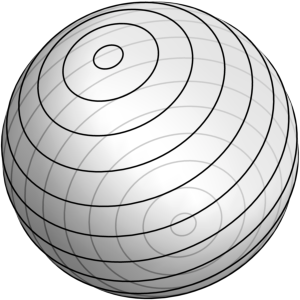
\includegraphics[width=.7\columnwidth]{figures/celestial-ball-1.pdf}
		\caption{Elliptical}
	\end{subfigure}
	\vskip3ex
	\begin{subfigure}{\columnwidth}
		\centering
		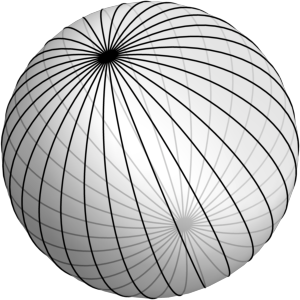
\includegraphics[width=.7\columnwidth]{figures/celestial-ball-2.pdf}
		\caption{Hyperbolic}
	\end{subfigure}
	\vskip3ex
	\begin{subfigure}{\columnwidth}
		\centering
		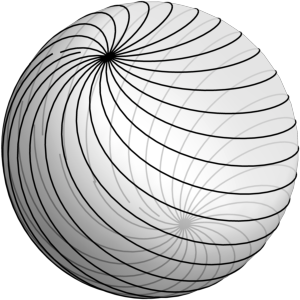
\includegraphics[width=.7\columnwidth]{figures/celestial-ball-3.pdf}
		\caption{Loxodromic}
	\end{subfigure}
	\caption{
		Lorentz transformations on the celestial sphere, taking curves to themselves.
	}
	\label{fig:celestial-balls}
\end{marginfigure}


Elliptical Lorentz transformations are \emph{rotations}, whose rotors are generated by spacelike $2$-blades; hyperbolic transformations are \emph{boosts}, with timelike $2$-blades generators.
Parabolic transformations are sometimes called \emph{null rotations}, and fall in between the previous two, with null $2$-blades as generators.

The final class of loxodromic transformations are a combination of a rotation and a boost where the axis of rotation is parallel with the boost direction (in a particular frame).
A loxodromic generator is \emph{not} a $2$-blade, but a bivector comprising mutually $2$-orthogonal\sidenote{
	in the sense of \cref{def:Δ-orthogonal}, \cref{sec:higher-orthogonal}
} $2$-blades, one timelike and one spacelike.

These can be helpfully visualised by making use of the isomorphism $\SO^+(1,3) \cong \op{Aut}(\CC \cup \set{∞})$ of the Lorentz group with the Möbius group of conformal transformations on the sphere.
An observer undergoing a change of frame will see the celestial sphere transform conformally, as in \cref{fig:celestial-balls}.

\chapter{Composition of Rotors in terms of their Generators}


In studying proper orthogonal transformations, it is often easier to represent them in terms of their generators $σ_i ∈ \GA(p,q)$ which belong to the Lie algebra $\liealg{so}(p,q)$.
A fundamental question is how such transformations compose in terms of these generators: ``given $σ_1$ and $σ_2$, what is $σ_3$ such that $e^{σ_1}e^{σ_2} = e^{σ_3}$?''
This is of theoretical interest and is useful practically when representing transformations in terms of their generators is cheaper.
One may use the \x{BCH full}\sidenote{
	Often simply Baker--Campbell--Hausdorff and permutations thereof.
} (\x{BCH}) formula $\bch{σ_1}{σ_2} ≔ \log(e^{σ_1}e^{σ_2})$ which is well studied in general Lie theory \cite{achilles2012bch-early}.
However, the general \x{BCH} formula
\begin{align}
	\bch{a}{b} = a + b + \frac12[a, b] + \frac{1}{12}[a, [a, b]] + \frac{1}{12}[[a, b], b] + \cdots
	\label{eqn:general-BCH-formula}
\end{align}
involves an infinite series of nested commutators and may not obviously admit a useful closed form.

In the case of Lorentz transformations $\SO^+(1,3)$, some closed-form expressions for \cref{eqn:general-BCH-formula} have been found using a $2$-form representation of $\liealg{so}(1,3)$ \cite{coll2002sr-generator-composition,coll1990sr-generator-exponentiation}, but the expressions are complicated and do not clearly reduce to well-known formulae in, for example, the special cases of pure rotations or pure boosts.
The rotor formalism of geometric algebra leads to an elegant closed form of \cref{eqn:general-BCH-formula} which, in the case of Lorentzian spacetime, is inexpensive to compute.




\section{A Geometric \x{BCH} Formula}
\label{sec:bch-derivation}

Suppose $σ ∈ \GA[2](p, q)$ is a bivector in a geometric algebra of dimension $p + q ≤ 4$.
By their definitions as formal power series, we have
\begin{math}
	e^{σ} = \cosh σ + \sinh σ
,\end{math}
where `$\cosh$' involves even powers of $σ$ and `$\sinh$' odd powers.
For convenience, define the linear projections onto \textdef{self-reverse} and \textdef{anti-self-reverse} parts respectively as
\begin{align}
	\srev{A} &≔ \frac12\qty(A + \rev{A})
&	&\text{and}
&	\arev{A} &≔ \frac12\qty(A - \rev{A})
	\label{eqn:rev-notation}
.\end{align}
Since any bivector obeys $\rev{σ} = -σ$, it follows that $\rev{(e^σ)} = e^{-σ} = \cosh σ - \sinh σ$.
Using the notation \eqref{eqn:rev-notation}, the self-reverse and anti-self-reverse projections of $e^σ$ are $\srev{e^{σ}} = \cosh σ$ and $\arev{e^{σ}} = \sinh σ$, respectively.
Furthermore, these two projections commute, and so
\begin{align}
	{\arev{e^{σ}}}{\srev{e^{σ}}}^{-1}
	= {\srev{e^{σ}}}^{-1}{\arev{e^{σ}}}
	= \frac{\arev{e^{σ}}}{\srev{e^{σ}}}
	= \tanh σ
\end{align}
which leads to an expression for the logarithm of any rotor $\rotor R = ± e^σ$.
\begin{align}
	σ = \log(\rotor R) = \arctanh\qty(\frac{\arev{\rotor R}}{\srev{\rotor R}})
	\label{eqn:log-rotor}
\end{align}
Note that the overall sign of the rotor is not recovered, and $\log(+\rotor R) = \log(-\rotor R)$ according to \cref{eqn:log-rotor}.
However, this does not affect the Lorentz transformation $\lin R ∈ \SO^+(p, q)$, since it is defined by $R(𝒖) = \rotor R𝒖\rev{\rotor R}$.
The exact sign can be recovered by considering the relative signs of $\arev{\rotor R}$ and $\srev{\rotor R}$, as in \cite[§\,5.3]{lasenby2011ga-practical}.


From \cref{eqn:log-rotor} we may derive a \x{BCH} formula by substituting $\rotor R = e^{σ_1}e^{σ_2}$ for any two bivectors $σ_i ∈ \GA[2](p, q)$.
Using the shorthand $\Co{i} ≔ \cosh σ_i$ and $\Si{i} ≔ \sinh σ_i$, the composite rotor is
\begin{align}
	\rotor R = e^{σ_1}e^{σ_2}
	= (\Co1 + \Si1)(\Co2 + \Si2)
	= \Co1\Co2 + \Si1\Co2 + \Co1\Si1 + \Si1\Si2
.\end{align}
For $p + q < 4$, any even function of a bivector (such as $\Co{i}$) is a scalar, and for $p + q = 4$, is a $\qty{0,4}$-multivector $α + β\vol$.
In either case, the $\Co{i}$ commute with even multivectors, so $[\Co{i}, \Co{j}] = [\Co{i}, \Si{j}] = 0$.
Therefore, the self-reverse and anti-self-reverse parts are
\begin{align}
	\srev{\rotor R} &= \Co1\Co2 + \frac12\qty{\Si1, \Si2}
&	&\text{and}
&	\arev{\rotor R} &= \Si1\Co2 + \Co1\Si2 + \frac12\qty[\Si1, \Si2]
	\label{eqn:arev-and-srev-parts}
.\end{align}
Hence, from \cref{eqn:log-rotor} we obtain an explicit \x{BCH} formula.

\begin{theorem}[rotor \x{BCH} formula]
	\label{thm:geometric-BCH}
	If $σ_1, σ_2 ∈ \GA[2](p, q)$ are bivectors in $p + q ≤ 4$ dimensions, then $e^{σ_1}e^{σ_2} = ±e^{\bch{σ_1}{σ_2}}$ where
	\begin{align}
		\label{eqn:geometric-BCH}
		\bch{σ_1}{σ_2}
		% \coloneqq \log(e^{σ_1}e^{σ_2})
		= \arctanh\qty(\frac{
			\Ta1 + \Ta2 + \frac12\qty[\Ta1, \Ta2]
		}{
			1 + \frac12\qty{\Ta1, \Ta2}
		})
	\end{align}
	where we abbreviate $\Ta{i} \coloneqq \tanh σ_i$.
	Note that this satisfies the rotor equation with an overall ambiguity in sign.
\end{theorem}

We may wish to express \cref{eqn:geometric-BCH} in terms of geometrically significant products instead of \paren{anti}commutators.
A bivector product is generally a $\qty{0,2,4}$-multivector
\begin{align}
	ab
	&= \grade[0]{ab} + \grade[2]{ab} + \grade[4]{ab}
\\	&= a \fatdot b + a × b + a ∧ b
	\label{eqn:bivector-products}
.\end{align}
where $a×b = \grade[2]{ab} = \frac12[a, b]$ is the commutator product.
We may then write \cref{eqn:geometric-BCH} so that the grade of each term is explicit:
\begin{align}
	\bch{σ_1}{σ_2} = \arctanh\qty(\frac{
		\Ta1 + \Ta2 + \Ta1 × \Ta2
	}{
		1 + \Ta1 \fatdot \Ta2 + \Ta1 ∧ \Ta2 
	})
	\label{eqn:geometric-BCH-products}
\end{align}
The numerator is a bivector, while the denominator contains scalar ($\Ta1·\Ta2$) and $4$-vector ($\Ta1\wedge\Ta2$) terms.







\subsection{Zassenhaus-type formulae}

It is interesting to generalise the \x{BCH} formula \eqref{eqn:general-BCH-formula} to three rotors
\begin{math}
	e^{σ_1}e^{σ_2}e^{σ_3} = e^σ
\end{math}
in an algebra $\GA(p, q)$ with $p + q ≤ 4$.
A solution to this rotor equation is
\begin{align}
	σ = \log(±e^σ) = \arctanh\qty(\frac{\arev{e^{σ_1}e^{σ_2}e^{σ_3}}}{\srev{e^{σ_1}e^{σ_2}e^{σ_3}}})
,\end{align}
by \cref{eqn:log-rotor}.


We will find it convenient to define the \textdef{anticommutator product} $A\wedot B ≔ \frac12\qty{A, B}$ to complement the commutator product $A×B$.
The symbol ``$\wedot$'' is motivated by the fact that, for bivectors, we have
\begin{math}
	σ\wedot ρ = σ\cdot ρ + σ∧ρ
\end{math}
and thus
\begin{align}
	\label{eqn:(anti)com-prods}
	σ\wedot ρ &≔ \frac12(σρ + ρσ) = \srev{σρ}
,&	σ×ρ &≔ \frac12(σρ - ρσ) = \arev{σρ}
.\end{align}





Because $e^{σ_1}e^{σ_2}e^{σ_3} ∈ \GA[+](p, q)$ is an even multivector, the anti-self-reverse projection is exactly the bivector part,
\begin{math}
	\arev{e^{σ_1}e^{σ_2}e^{σ_3}} = \grade[2]{e^{σ_1}e^{σ_2}e^{σ_3}}
,\end{math} and the self-reverse projection is the $\set{0,4}$-multivector part.\sidenote{
	Recall $\rev{A} = \revsign{k}A$ for a $k$-vector $A$ where $(\etc{\revsign{\i}}{}4) = (++--{})$.
}
Decomposing $e^{σ_i} = \Co i + \Si i$, we find $2^3$ terms which separate into%
\begin{fullwidth}
	\begin{align}
		\arev{e^{σ_1}e^{σ_2}e^{σ_3}} &=
		% \grade[2]{e^{σ_1}e^{σ_2}e^{σ_3}} =
		\Si1\Co2\Co3 +
		\Co1\Si2\Co3 +
		\Co1\Co2\Si3 +
		(\Co1\Si2 + \Si1\Co2)×\Si3 +
		(\Si1×\Si2)\Co3 +
		\arev{\Si1\Si2\Si3} 
	,\\	\srev{e^{σ_1}e^{σ_2}e^{σ_3}} &=
		% \grade[0,4]{e^{σ_1}e^{σ_2}e^{σ_3}} =
		\Co1\Co2\Co3 +
		(\Co1\Si2 + \Si1\Co2) \wedot \Si3 +
		(\Si1\wedot\Si2) \Co3 +
		\srev{\Si1\Si2\Si3}
	.\end{align}
\end{fullwidth}
The $\set{0,4}$-multivectors $\Co i$ commute with the bivectors $\Si i$, and products of $\Co i$ and $\Si j$ are themselves bivectors.
Therefore, terms containing one $\Si i$ factor are bivectors, and terms containing two $\Si i$ factors, such as $\Si1\Si2\Co3$, are products of bivectors, or $\set{0, 2, 4}$-multivectors.
These terms are split into bivectors $(\Si1×\Si2)\Co3$ and $\set{0,4}$-multivectors $(\Si1\wedot\Si2)\Co3$.


Cancelling factors of $\Co1\Co2\Co3$, we then have
\begin{align}
	\label{eqn:ternary-bch.1}
	\frac{\arev{e^{σ_1}e^{σ_2}e^{σ_3}}}{\srev{e^{σ_1}e^{σ_2}e^{σ_3}}} =
	\frac{
		\Ta1 + \Ta2 + \Ta3 + (\Ta1 + \Ta2)×\Ta3 + \Ta1 × \Ta2 + \arev{\Ta1\Ta2\Ta3}
	}{
		1 + (\Ta1 + \Ta2)\wedot \Ta3 + \Ta1 \wedot \Ta2 + \srev{\Ta1\Ta2\Ta3}
	}
\end{align}
where $\Ta i ≔ \tanh σ_i$.
The next lemma is used to rewrite the rightmost terms with \paren{anti}commutator products \eqref{eqn:(anti)com-prods}.
\begin{lemma}
	For any bivectors $σ,ρ,ω ∈ \GA[2](p, q)$ where $p + q ≤ 4$,
	\begin{align}
		\arev{σρω} &= (σ\wedotρ)\wedotω + (σ×ρ)×ω
	,&	\srev{σρω} &= (σ×ρ)\wedotω
	.\end{align}
\end{lemma}
\begin{proof}
	Observe that $\arev{σρω} = \grade[2]{σρω}$ since $σρω$ is a $\set{0, 2, 4}$-multivector, of which only the bivector part is anti-self-reverse.
	Using associativity and linearity,
	\begin{align}
		\grade[2]{σρω} = \grade[2]{(σ\wedotρ)ω} + \grade[2]{(σ×ρ)ω} = (σ\wedotρ)ω + (σ×ρ)×ω
	.\end{align}
	The product $(σ\wedotρ)ω = (σ\wedot ρ)\wedot ω$ is between a $\set{0,4}$-multivector and a bivector, which may only contain bivector components.
	The product $(σ×ρ)ω$ is between two bivectors, having bivector part $(σ×ρ)×ω$.

	Similarly, note that
	\begin{align}
		\srev{σρω} = \grade[0,4]{(σ\wedotρ)ω} + \srev{(σ×ρ)ω} = (σ×ρ)\wedotω
	,\end{align}
	where the first term vanishes since $(σ\wedotρ)ω$ is a bivector.
\end{proof}

This allows us to collect the terms in \cref{eqn:ternary-bch.1} as
{\begin{align}
	\frac{\arev{e^{σ_1}e^{σ_2}e^{σ_3}}}{\srev{e^{σ_1}e^{σ_2}e^{σ_3}}}
	% &= \frac{
	% 	(\Ta1 + \Ta2 + \Ta1 × \Ta2) + \Ta3 + (\Ta1 + \Ta2 + \Ta1 × \Ta2)×\Ta3 + (\Ta1\wedot\Ta2)\wedot\Ta3
	% }{
	% 	1 + (\Ta1 + \Ta2 + \Ta1×\Ta2)\wedot \Ta3 + \Ta1 \wedot \Ta2
	% }
	&= \frac{
		\Ta{12} + \Ta3 + \Ta{12}×\Ta3 + (\Ta1\wedot\Ta2)\wedot\Ta3
	}{
		1 + \Ta{12}\wedot \Ta3 + \Ta1 \wedot \Ta2
	}
\end{align}}
where $\Ta{12} ≔ \Ta1 + \Ta2 + \Ta1×\Ta2$.
This leads us to the
\begin{theorem}
	For bivectors $σ_i ∈ \GA[2](p, q)$ with $p + q ≤ 4$,
	\begin{align}
		e^{σ_1 + σ_2} &= e^{σ_1}e^{σ_2}e^ρ
	\end{align}
	where
	\begin{align}
		ρ &= \arctanh\qty(\frac{
			F - R - R×F + S\wedot F
		}{
			1 - R\wedot F + S
		})
	,\\	F &= \tanh(σ_1 + σ_2)
	,\\	R &= \tanh(σ_1)×\tanh(σ_2) + \tanh(σ_1) + \tanh(σ_2)
	,\\	S &= \tanh(σ_1)\wedot\tanh(σ_2)
	.\end{align}
\end{theorem}

\todo{First order corrections? Don’t know where to go with this.}









\subsection{In low dimensions: Rodrigues' rotation formula}

It is illustrative to see how the \x{BCH} formula \eqref{eqn:geometric-BCH} reduces in low-dimensional special cases.
Indeed, in two dimensions, all bivectors are scalar multiples of $\vol = \ve_1\ve_2$, and we recover the trivial case $e^ae^b = e^{a+b}$. %$\bch{a}{b} = a + b$.
Specifically, in the Euclidean $\GA(2)$ plane (or anti-Euclidean $\GA(0,2)$ plane) we have $\vol^2 = -1$, and \cref{eqn:geometric-BCH} simplifies by way of the tangent angle addition identity
\begin{align}
	\arctan(\frac{\tan θ_1 + \tan θ_1}{1 - \tan θ_1 \tan θ_2}) = θ_1 + θ_2
.\end{align}
This identity encodes how angles add when given as the gradients of lines; $m = \tan θ$.

Similarly, in the hyperbolic plane $\GA(1,1)$ with basis $\set{\ve_+, \ve_-}, \ve_±^2 = ±1$, the pseudoscalar $\vol = \ve_+\ve_-$ generates \emph{hyperbolic} rotations $e^{\vol ξ} = \cosh ξ + \vol\sinh ξ$ owing to the fact that $\vol^2 = -\ve_+^2\ve_-^2 = +1$.
Then, \cref{eqn:geometric-BCH} simplifies by the hyperbolic angle addition identity
\begin{align}
	\arctanh\qty(\frac{\tanh ξ_1 + \tanh ξ_1}{1 + \tanh ξ_1 \tanh ξ_2}) = ξ_1 + ξ_2
\end{align}
which encodes how collinear rapidities add when given as relativistic velocities; $β = \tanh ξ$.

Less trivially, a rotation in $\RR^3$ by $θ$ may be represented by its \textdef{Rodrigues vector}\sidenote{
	Olinde Rodrigues first originated the formula in 1840 \cite[pp. 406]{rodrigues1840rotations}.
} $\vb r = \vb{\hat{r}}\tan\fracθ2$ pointing along the axis of rotation.
The composition of two rotations is then succinctly encoded in Rodrigues' composition formula
\begin{align}
	\vb r_{12} = \frac{\vb r_1 + \vb r_2 - \vb r_1 × \vb r_2}{1 - \vb r_1 · \vb r_2}
	\label{eqn:rodrigues-formula}
\end{align}
involving the standard vector dot and cross products.

We can easily derive \cref{eqn:rodrigues-formula} as a special case of \cref{eqn:geometric-BCH-products} as follows:
Let $σ_1, σ_2 ∈ \GA[2](3)$ be two bivectors defining the rotors $e^{σ_1}$ and $e^{σ_2}$ in three dimensions.
In $\GA(3)$, the only $4$-vector is trivial, so $σ_1 ∧ σ_2 = 0$ and for the composite rotor $e^{σ_3} \coloneqq e^{σ_1}e^{σ_2}$ we have
\begin{align}
	σ_3 = \bch{σ_1}{σ_2} = \arctanh\qty(\frac{
	\tanh σ_1 + \tanh σ_2 + \tanh σ_1 \times \tanh σ_2
	}{
	1 + \tanh σ_1 · \tanh σ_2
	})
\end{align}
where $a × b$ is the commutator product of bivectors as in \cref{eqn:bivector-products}, not the vector cross product.
Observe that Euclidean bivectors $σ_i ∈ \GA[2](3)$ have negative square (e.g., $(\ve_1\ve_2)^2 = -\ve_1^2\ve_2^2 = -1$) and relate to their dual normal vectors by $\vb{u}_i$ by $σ_i = \vb{u}_i\vol$.
Therefore, by rewriting
\begin{math}
	\tanh σ_i
	= \tanh (\vb{u}_i\vol)
	= (\tan \vb{u}_i)\vol
,\end{math}
we obtain the formula in terms of plain vectors and the vector cross product.
\begin{align}
	\vb{u}_{12} = (\bch{\vb{u}_1\vol}{\vb{u}_2\vol})\vol^{-1}
	= \arctan\qty(\frac{
	\tan \vb{u}_1 + \tan \vb{u}_2 - \tan \vb{u}_1 \times \tan \vb{u}_2
	}{
	1 - \tan \vb{u}_1 · \tan \vb{u}_2
	})
\end{align}
Indeed, a bivector $σ_i = \vb{u}_i\vol$ generates an $\RR^3$ rotation through an angle $θ = 2\|\vb{u}_i\|$ via the double-sided transformation law
\begin{math}
	a \mapsto e^{\vb{u}\vol}ae^{-\vb{u}\vol}
.\end{math}
Hence, $\tan \vb{u}_i = \vb{\hat{v}}_i\tan\fracθ2 ≡ \vb{r}_i$ are exactly the half-angle Rodrigues vectors, and we recover \cref{eqn:rodrigues-formula}.

The necessity of the half-angle in the Rodrigues vectors reflects the fact that they actually generate \emph{rotors}, not direct rotations, and hence belong to the underlying spin representation of $\SO^+(3)$ --- a fact made clearer in the context of geometric algebra.









\subsection{In higher dimensions}

In fewer than four dimensions, the $4$-vector $\Ta1\wedge\Ta2 = 0$ appearing in the geometric \x{BCH} formula is trivial, and so \cref{eqn:geometric-BCH} involves only bivector addition and scalar multiplication.
In four dimensions, there is one linearly independent $4$-vector --- the pseudoscalar --- which necessarily commutes with all even multivectors.
However, in more than four dimensions, $4$-vectors do \emph{not} necessarily commute with bivectors, and the assumptions underlying \cref{eqn:arev-and-srev-parts} and hence the main result \eqref{eqn:geometric-BCH} fail.


On the face of it, the \x{BCH} formula \eqref{eqn:geometric-BCH} in the four-dimensional case appears deceptively simple --- it hides complexity in the calculation of the trigonometric functions of arbitrary bivectors,
\begin{fullwidth}
	\begin{align}
		\tanh σ_i &= σ - \frac13σ^3 + \frac{2}{15}σ^5 + \cdots
	&	&\text{and}
	&	\arctanh σ_i &= σ +\frac13σ^3 + \frac15σ^5 + \cdots
		\label{eqn:trig-power-series}
	.\end{align}
\end{fullwidth}

In fewer dimensions, $σ^2$ is a scalar, and so these power series are as easy to compute as their real equivalents.\sidenote{
	If $σ^2 = N_σ^2 ∈ \RR$, then we have simply $\tanh σ = (\tanh N_σ)N_σ^{-1}σ$.
}
But in four dimensions, $σ^2$ is in general a $\qty{0,4}$-multivector (by lemma~\ref{lem:grades-of-square}) and the power series \eqref{eqn:trig-power-series} are more complicated.
However, if $σ^2 \ne 0$ has a square root $N_σ = α + β\vol$ in the scalar--pseudoscalar plane, then one has $σ = N_σ\hat{σ} = \hat{σ}N_σ$ where $\hat{σ} \coloneqq σ/N_σ$ so that $\hat{σ}^2 = 1$.
With a bivector $σ = N_σ\hat{σ}$ expressed in this form, the valuation of a formal power series $f(z) = \sum_{n=1}^\infty f_n z^n$ simplifies to
\begin{align}
\label{eqn:normalised-power-series}
	\text{($f$ even)}&
&	f(σ) &= \sum_{n = 1}^\infty f_{2n} σ^{2n}
	= \sum_{n = 1}^\infty f_{2n} N_σ^{2n}
	= f(N_σ)
,\\	\text{($f$ odd)}&
&	f(σ) &= \sum_{n = 1}^\infty f_{2n + 1} σ^{2n + 1}
	= \sum_{n = 1}^\infty f_{2n} N_σ^{2n + 1} \hat{σ}
	= f(N_σ)\hat{σ}
.\end{align}
This is especially useful in the case of Minkowski spacetime $\GA(1,3)$ because the scalar--pseudoscalar plane is isomorphic to $\CC$ and square roots always exist (see \cref{sec:invariant-bivector-decomposition}).
From now on, we focus on the special case of Minkowski spacetime, and consider practical and theoretical applications.








\section{\x{BCH} Composition in Spacetime}

Because the geometric \x{BCH} formula is constructed from sums and products of bivectors, it involves only even spacetime multivectors.
Therefore, in numerical applications, it is not necessary to represent the full STA, but only the even subalgebra $\GA[+](1,3) \cong \GA(3)$.

The algebra of physical space $\GA(3)$ admits a faithful complex linear representation by the Pauli spin matrices \cite{baylis1989sta-pauli,lasenby2016ga-unified-language,hestenes2003sta}.
The real dimension of both $\CC^{2×2}$ and $\GA(3)$ is eight, so there is no redundancy in the Pauli representation, so it is convenient for computer implementation.



An even $\GA[+](1,3)$ multivector --- or equivalently, a general $\GA(3)$ multivector --- may be parametrised by four complex scalars $q^μ = \Re(q^μ) + i\Im(q^μ) ∈ \CC$ as
\begin{align}
	A = \Re(q^0) + \Re(q^i)\vs_i + \Im(q^i)\vol\vs_i + \Im(q^0)\vol
,\end{align}
where the $\vs_i$ may be read both as spacetime bivectors $\vs_i \equiv \vg_0\vg_i ∈ \GA[+](1,3)$ or as basis vectors of $\GA(3)$ under a space/time split.
The Pauli matrices $σ_i ∈ \CC^{2×2}$ form a linear representation of $\GA(3)$ by the association $\vs_i \equiv σ_i$.
Explicitly, identifying
\begin{align}
	\vs_1 &\equiv \mqty[
		 0&+1\\
		+1& 0\\
	]
&	\vs_2 &\equiv \mqty[
		 0&-i\\
		+i& 0\\
	]
&	\vs_3 &\equiv \mqty[
		+1& 0\\
		 0&-1\\
	]
\end{align}
along with $1 \equiv I$ and $\vol \equiv iI$ where $I$ is the identity matrix, we obtain a representation of the multivector $A$ by a $2 × 2$ complex matrix:
\begin{align}
	\lin A \equiv \mqty[
		q^0 + q^3 & q^1 - iq^2 \\
		q^1 + iq^2 & q^0 - q^3
	]
	\label{eqn:multivector-as-matrix}
.\end{align}






A proper Lorentz transformation $\lin Λ ∈ \SO^+(1,3)$ is determined in the $K$ frame by a vector rapidity $\vb ξ ∈ \RR^3$ and axis-angle vector $\vb θ ∈ \RR^3$.
The standard $4×4$ matrix representation of $\lin Λ$ is obtained as the exponential of the generator
\begin{align}
	\mqty[
		 0 &  \vb ξ^T \\
		\vb ξ & ε_{ijk}θ^k
	] =
	\qty[\begin{array}{llll}
	0 & \phantom{±}ξ^1 & \phantom{±}ξ^2 & \phantom{±}ξ^3 \\
	ξ^1 & \phantom{±}0 & +θ^3 & -θ^2 \\
	ξ^2 & -θ^3 & \phantom{±}0 & +θ^1 \\
	ξ^3 & +θ^2 & -θ^1 & \phantom{±}0
	\end{array}]
	\in \liealg{so}(1,3)
	\label{eqn:lorentz-generator-matrix}
.\end{align}
In the spin representation, the transformation $\lin Λ$ corresponds to a rotor $\rotor L = e^σ$, and the generating bivector \eqref{eqn:bivector-generator} may be expressed via \cref{eqn:multivector-as-matrix} as the traceless complex matrix
\begin{align}
	\lin Σ = q^kσ_k = \mqty[
		+q^3 & q^1 - iq^2 \\
		q^1 + iq^2 & -q^3
	]
	\label{eqn:bivector-as-matrix}
,\end{align}
where $q^k \coloneqq \frac12(ξ^k + iθ^k) ∈ \CC$.
% This represents the restriction of \eqref{eqn:multivector-as-matrix} to spacetime bivectors.
Note that, since the square of a spacetime bivector is a $\qty{0,4}$-multivector, its representative matrix $\lin Σ$ squares to a complex scalar multiple of the identity.



Given two generators $σ_i$ with matrix representations $\lin Σ_i$, the geometric \x{BCH} formula \eqref{eqn:geometric-BCH} reads
\begin{align}
	\lin Σ_3 ≔ \bch{\lin Σ_1}{\lin Σ_2} = \tanh^{-1}\qty(
		\lin{\frac{ T_1 + T_2 + A }{ I + S }}
	)
	\label{eqn:matrix-BCH}
,\end{align}
where $\lin T_i ≔ \tanh \lin Σ_i$.
To efficiently compute $\lin T_i$, make use of the fact that $\lin Σ_i^2 = λ_i^2\lin I$ is a complex multiple of the identity matrix and evaluate $\lin T_i = (\tanh λ_i)λ_i^{-1}\lin Σ_i$.
In the null case $\lin Σ_i^2 = λ = 0$, we have trivially $\tanh \lin Σ_i = \lin Σ_i = \tanh^{-1} \lin Σ_i$.



The commutator $\lin A ≔ \frac12[\lin T_1, \lin T_2]$ and anti-commutator $\lin S ≔ \frac12\qty{\lin T_1, \lin T_2}$ terms may be efficiently computed by separating the single matrix product $\lin{ Π ≔ T_1T_2 = A + S }$ into off-diagonal and diagonal components, respectively; i.e.,
\begin{align}
	\lin A_{ij} = (1 - δ_{ij})\lin Π_{ij}
	\qqtext{and}
	\lin S_{ij} = δ_{ij}\lin Π_{ij}
.\end{align}
The numerator of \cref{eqn:matrix-BCH} is therefore a matrix with zeros on the diagonal, and the denominator is a complex scalar multiple of the identity, so the argument of $\tanh^{-1}$, call it $\lin M$, is in the form \eqref{eqn:bivector-as-matrix}.
Computing $\tanh^{-1} \lin M$ again simply amounts to
\begin{math}
	\lin Σ_3 = \tanh^{-1} \lin M = (\tanh^{-1} λ)λ^{-1}\lin M
\end{math}
where $\lin M^2 = λ^2\lin I$.

The Lorentz generator in the standard vector representation \eqref{eqn:lorentz-generator-matrix} can then be recovered from $\lin Σ_3$ with the relations $ξ^k = 2\Re(q^k)$ and $θ^k = 2\Im(q^k)$, and the final $\SO^+(1,3)$ vector transformation is its $4×4$ matrix exponential.









\subsection{Relativistic 3-velocities \& the Wigner Angle}

As an example of its theoretical utility, we shall use the geometric \x{BCH} formula \eqref{eqn:geometric-BCH} to derive the composition law for arbitrary relativistic $3$-velocities.

The innocuous problem of composing relativistic velocities has been called ``paradoxical'' \cite{ungar1989sr-velocity-composition,mocanu1992sr-velocity-composition,visser2011sr-velocity-composition}, owing in part to the fact that \emph{irrotational} boosts are not closed under composition, and that explicit matrix analysis becomes cumbersome.
Of course, in reality there is no paradox, and the full description of the composition of boosts is pedagogically valuable as it highlights aspects of special relativity which differ from spatial intuition.


We may speak of a rotation or boost as being \textdef{pure} relative to the $K$ frame.
Technically, $σ$ generates a pure rotation (or pure boost) if, under the space/time split relative to the $K$ frame, $σ = \grade[2]{σ}$ is a pure bivector (or a pure vector) in $\GA(3)$.
A pure rotation or pure boost relative to $K$ is \emph{not} pure in all other frames.

The restriction of the \x{BCH} formula to pure boosts is not as simple as the restriction to rotations \eqref{eqn:rodrigues-formula}, because pure boosts do not form a closed subgroup of $\SO^+(1,3)$ as pure rotations do.
Instead, the composition of two pure boosts $\rotor B_i$ is a pure boost composed with a pure rotation (or vice versa),
\begin{align}
	\rotor B_1\rotor B_2 = \rotor B\rotor R
	\label{eqn:boost-boost-makes-boost-rotation}
.\end{align}
The direction of the boost $\rotor B$ lies within the plane defined by the boost directions of $\rotor B_1$ and $\rotor B_2$, and $\rotor R$ is a rotation through this plane by the \emph{Wigner angle} \cite{visser2011sr-velocity-composition}.
Applying \cref{eqn:geometric-BCH} to this case immediately yields formulae for the resulting boost and rotation.\sidenote{
	These results are equivalent to those in \cite{berry2020quat-sr} which are formulated using complexified quaternions.
}



For ease of algebra, we conduct the following analysis under a space/time split with respect to the $K$ frame.
Under this split, a pure boost $\rotor B$ is generated by an $\RR^3$ vector $\frac{\vb ξ}{2}$, and a pure rotation $\rotor R$ is generated by an $\RR^3$ bivector $\fracθ2\hat{r}$.
Here, $\vb ξ ∈ \GA[1](3)$ is the \emph{vector rapidity}, related to the velocity by $\vb v/c = \vb β = \tanh \vb ξ$, and the rotation is through an angle $θ$ in the plane spanned by the bivector $\hat{r} ∈ \GA[2](3)$.
\Cref{eqn:geometric-BCH} with two pure boosts $\vb ξ_1$ and $\vb ξ_2$ is
\begin{align}
	\tanh(\bch{\frac{\vb ξ_1}{2}}{\frac{\vb ξ_2}{2}})
	= \frac{𝒘_1 + 𝒘_2 + 𝒘_1 ∧ 𝒘_2}{1 + 𝒘_1⋅𝒘_2}
	\label{eqn:boost-boost}
\end{align}
where $𝒘_i ≔ \tanh\frac{\vb ξ_i}{2}$ are the \emph{relativistic half-velocities}, also defined in \cite{berry2020quat-sr,berry2021quat-sr}.
The generator \eqref{eqn:boost-boost} has vector and bivector (namely $𝒘_1 ∧ 𝒘_2$) parts, indicating that the Lorentz transformation it describes is indeed some combination of a boost and a rotation.


Similarly, for an arbitrary pure boost and pure rotation,
\begin{align}
	\tanh(\bch{\frac{\vb ξ}2}{\fracθ2\hat{r}})
	= \frac{𝒘 + ρ + \frac12[𝒘, ρ]}{1 + 𝒘\wedge ρ}
	\label{eqn:boost-rotation}
\end{align}
where $ρ ≔ \tanh \frac{θ\hat{r}}2 = \hat{r}\tan\frac θ2$ is a bivector.
In general, \cref{eqn:boost-rotation} has vector, bivector \emph{and} pseudoscalar parts (the commutator $\frac12[𝒘, ρ] = \grade[1]{𝒘ρ} + 𝒘 \wedge ρ$ and the denominator both have grade-three part $𝒘\wedge ρ$).
However, \cref{eqn:boost-boost,eqn:boost-rotation} are equal by supposition of \cref{eqn:boost-boost-makes-boost-rotation}.
By comparing parts of equal grade, we deduce the pseudoscalar part of \cref{eqn:boost-rotation} is zero.
This requires $𝒘\wedge ρ = 0$ or, equivalently, that $𝒘$ lies in the plane defined by $ρ$ --- meaning the resulting boost is coplanar with the Wigner rotation as expected.
Hence, for a coplanar boost and rotation, \cref{eqn:boost-rotation} is simply
\begin{align}
	\tanh(\bch{\frac{\vb ξ}2}{\fracθ2\hat{r}})
	= 𝒘 + ρ + 𝒘ρ
	\label{eqn:boost-rotation-coplanar}
.\end{align}
The term $𝒘ρ = \grade[1]{𝒘ρ} = -ρ𝒘$ is a vector orthogonal to $𝒘$ in the plane defined by $ρ$.




Equating the bivector parts of \cref{eqn:boost-boost,eqn:boost-rotation-coplanar} determines the rotation
\begin{align}
	ρ &= \frac{𝒘_1 \wedge 𝒘_2}{1 + 𝒘_1 · 𝒘_2}
,&	&\text{implying}
&	θ = 2\tan^{-1}\qty(\frac{w_1w_2\sinϕ}{1 + w_1w_2\cosϕ})
\end{align}
where $ϕ$ is the angle between the two initial boosts (in the $K$ frame).
The angle $θ$ is precisely the Wigner angle.
Equating the vector parts determines the boost
\begin{align}
	𝒘 &= \frac{𝒘_1 + 𝒘_2}{1 + 𝒘_1⋅𝒘_2}(1 + ρ)^{-1}
,\end{align}
noting that $𝒘_i$ and $ρ$ do not commute.
Substituting $ρ$ leads to the remarkably succinct composition law
\begin{math}
	𝒘 = (𝒘_1 + 𝒘_2)(1 + 𝒘_1𝒘_2)^{-1}
\end{math}
exhibited in \cite{berry2020quat-sr}, with the final relativistic velocity being $\vb β = \tanh \vb ξ = \tanh (2\tanh^{-1} 𝒘)$.


\chapter{Calculus in Flat Space(time)}

So far, we have been concerned with special relativity at a single point in spacetime.
The simplest first step toward a description of quantities extending across regions (i.e., fields) is the assumption of \emph{flat spacetime}.
This is the statement that
\begin{itemize}
	\item points in spacetime are elements of a vector space $V$, and the difference of points is physically meaningful; and
	\item fields are parametric functions of a point in spacetime.
\end{itemize}
These assumptions are acceptable in special relativity.
But in arbitrary regions and in the presence of gravity, spacetime is curved and does not admit a meaningful vector space structure.
This leads to differential geometry and forms \cref{part:2}.

\begin{definition}
	A \textdef{field} $F$ in a flat space $V$ is a differentiable function with domain $V$.
\end{definition}


\todo{
	\begin{enumerate}
		\item Exterior derivative and vector derivative
		\item Stokes' theorem and the GA equivalent
		\item Maxwell's equations
	\end{enumerate}
}

\section{Differentiation}


The directional derivative of a field $F : V → A$ in the direction $𝒖 ∈ V$ is
\begin{align}
	% ∂_𝒖 F(x) = \lim_{ε → 0}\frac{F(x + ε𝒖) - F(x)}{ε}
	∂_𝒖 F(x) = \dv{ε} \eval{F(x + ε𝒖)}_{ε = 0}
	= \lim_{ε → 0}\frac{F(x + ε𝒖) - F(x)}{ε}
\end{align}
where the point $x ∈ V$ is also a vector.
The directional derivative is linear in $𝒖$, since by a change of variables,
\begin{math}
	∂_{u^a\ve_a}
	= \sum_a \dv{ε} \eval{F(x + εu^a\ve_a)}_{ε = 0}
	= \sum_a u^a \dv{ε'} \eval{F(x + ε'\ve_a)}_{ε' = 0}
	= u^a ∂_{\ve_a}
.\end{math}


Suppose $F : V → A$ is some algebra valued field.
It is useful to define a kind of ``total'' derivative $\DD F$ which does not depend on a direction of differentiation, but instead encompasses, in a sense, all derivatives into a single object $\DD F : V → A$.
The motivation for this construction is that it includes the soon-to-be-defined exterior derivative (of exterior algebra) and the vector derivative (of geometric algebra) as special cases.
This derivative will be defined when there is a canonical inclusion $ι : V^* → A$ of dual vectors into the algebra $A$, which is true if $A$ is a quotient if $\TA{(V^*)}$.

\begin{definition}
	\label{def:algder}
	Let $F : V → A$ be a field with values in an algebra $A$ with product $⊛$, equipped with an inclusion $ι : V^* → A$.
	The \textdef{algebraic derivative} of $F$ is
	\begin{align}
		\DD F ≔ ι(\ve^a) ⊛ ∂_{\ve_a} F
	\end{align}
	where $\set{\ve_a} ⊂ V$ and $\set{\ve^a} ⊂ V^*$ are dual bases (summation over $a$).
\end{definition}

\subsection{The Exterior Derivative}

An exterior form field $φ : V → \forms(V, U)$ is called an exterior \emph{differential} form ...

\subsection{The Vector Derivative}
\subsection{Case Study: Maxwell's Equations}


\section{Integration}


\subsection{Stokes' Theorem for Exterior Calculus}

\begin{theorem}[Stokes' theorem in $\RR^n$]
	\label{thm:flat-stokes}
	If $R ⊆ \RR^n$ is a compact $k$-dimensional hypersurface with boundary $∂R$, then a smooth differential form $ω ∈ \forms[k - 1](R)$ satisfies
	\begin{align}
		\label{eqn:stokes}
		\int_R \dd ω = \int_{∂R} ω
	.\end{align}
\end{theorem}
\begin{proof}
	Since $R$ is a $k$-dimensional region with boundary, every point $x ∈ R$ has a neighbourhood diffeomorphic to a neighbourhood of the origin in either $\RR^k$ or $H^k ≔ [0, ∞) ⊕ \RR^{k - 1}$, depending on whether $x$ is an interior point or a boundary point, respectively.

	\begin{marginfigure}
		\centering
		\includefigure[\columnwidth]{stokes-theorem}
		\caption{
			Neighbourhoods in $R$ are diffeomorphic either to interior balls or boundary half-balls.
		}
		\label{fig:stokes-theorem}
	\end{marginfigure}

	Let $\set{U_i}$ be a cover of $R$ consisting of such neighbourhoods.
	Since $R$ is compact, we may assume $\bigcup_{i=1}^N \set{U_i} = R$ to be a finite covering.
	Thus, we have finitely maps $h_i : U_i → X$ where $X$ is either $\RR^k$ or the half-space $H^k$, where $U_i \cong h_i(U_i)$ are diffeomorphic (see \cref{fig:stokes-theorem}).

	Finally, let $\set{ϕ_i : R → [0, 1]}$ be a partition of unity subordinate to $\set{U_i}$, so that $\set{x ∈ R | ϕ_i(x) > 0} ⊆ U_i$ and $ω = \sum_{i=1}^N ϕ_iω$.
	We need only prove the equality \eqref{eqn:stokes} for each $ω_i ≔ ϕ_iω$, and the full result follows be linearity.
	
	The form $h_i^*ω_i ∈ \forms[k - 1](X)$ can be written with respect to canonical coordinates of $X$ as
	\begin{align}
		h_i^*ω_i = \sum_{j=1}^k f_j (-1)^{j - 1} \dd x^{1\cdots\hat{j}\cdots k}
	\end{align}
	using the multi-index notation $\dx^{\etc{i_\i}{}k} ≡ \etc{\dx^{i_\i}}∧k$, where the hat denotes an omitted term.
	The factor of $(-1)^{j - 1}$ gives the $(k - 1)$-form the boundary orientation induced by the volume form $\dx^{\etc\i{}k}$ for convenience.
	Since pullbacks commute with $\dd$,
	\begin{align}
		h^*\ddω_i = \dd(h_i^*ω_i) = \sum_{j=1}^k \pdv{f_j}{x^j} \dd x^{1\cdots n}
	.\end{align}
	There are then two cases to consider.
	\begin{itemize}
		\item \emph{Interior case.}
		If $h_i : U_i → \RR^k$, then the right-hand side of \cref{eqn:stokes} vanishes because $ω_i$ is zero outside the neighbourhood $U_i ⊂ R$ which nowhere meets the boundary $∂R$.
		\begin{align}
			\int_{∂R} ω_i = \int_{∂U_i} ω_i = \int_∅ ω_i = 0
		\end{align}
		The left-hand side evaluates to
		\begin{align}
			\int_R \dd ω_i
			&= \int_X \dd (h_i^*ω_i)
			= \int_{\RR^k} \sum_{j=1}^k \pdv{f_j}{x^j} \dd x^{1\cdots n}
		\\	&= \underbrace{\etc{\int_{-∞}^{+∞}}{}{}}_k \sum_{j=1}^k \pdv{f_j}{x^j} \etc{dx^\i}{}{k}
		\\	&= \underbrace{\etc{\int_{-∞}^{+∞}}{}{}}_{k - 1} \sum_{j=1}^k \eval{f_j}_{x^j=-∞}^{+∞} (-1)^{j-1} dx^1\cdots\widehat{dx^j}\cdots dx^k
			= 0
		,\end{align}
		which vanishes because $h_i^*ω_i$, and hence the $f_j$, vanish outside the neighbourhood $h_i(U_i) ⊂ \RR^k$.

	\item \emph{Boundary case.}
	If $h_i : U_i → H^k$, then the boundary $∂U_i ⊂ ∂R$ is mapped onto the hyperplane $∂H^k = \set{(0, \etc[2]{x^\i},k) | x^j ∈ \RR}$.
	Thus, $dx^1 = 0$ on this boundary, and the right-hand side of \cref{eqn:stokes} becomes
	\begin{align}
		\int_{∂R}ω_i
		&= \int_{∂U_i} h_i^*ω_i
		= -\int_{\RR^{k - 1}} f_1 \etc[2]{dx^\i}{}k
	\\	&= -\underbrace{\etc{\int_{-∞}^{+∞}}{}{}}_{k - 1} f_1(0, \etc[2]{x^\i},k) \etc[2]{dx^\i}{}k
	.\end{align}
	The factor of $-1$ comes from the induced orientation of the boundary $∂H^k$, which is outward-facing, so in the \emph{negative} $x^1$ direction.
	For the left-hand side of \cref{eqn:stokes},
	\begin{align}
		\int_R \dd ω_i
		&= \int_{H^k} h_i^*\ddω_i
		= \int_0^∞ \etc{\int_{-∞}^{+∞}}{}{} \sum_{j=1}^k \pdv{f_j}{x^j} \etc{dx^\i}{}k
	\intertext{
		All terms $\pdv{f_j}{x^j}dx^j$ in the sum for $j > 1$ integrate to boundary terms $x_j → ±∞$ where $f_j$ vanishes.
		This leaves the single term from the integration of $dx^1$,
	}
		&= -\etc{\int_{-∞}^{+∞}}{}{} \eval{f_1}_{x^1=0}^∞ \etc[2]{dx^\i}k
	.\end{align}

	\end{itemize}

	Thus, we have equality for all $ω_i$, so
	\begin{align}
		\int_R \dd ω = \sum_{i=1}^N \int_R \dd ω_i = \sum_{i=1}^N \int_{∂R} ω_i = \int_{∂R} ω
	\end{align}
	by linearity.
\end{proof}

\subsection{Fundamental Theorem of Geometric Calculus}

\part{Geometry on Manifolds}
\label{part:2}

\chapter{Spacetime as a Manifold}






Here we only give a pragmatic definition of a manifold as a space which locally looks like $\RR^n$ upon which one can do calculus.
(More rigour can be found in the first chapter of \cite{lee2012diffgeo}.)
\begin{definition}
	\label{def:manifold}
	A \textdef{manifold $\manif M$ of dimension $n$} is a nice\sidenote{
		Here, a `nice' topological space is:
		\begin{enumerate}[leftmargin=1.3em]
		\item \emph{Hausdorff}, meaning each distinct pair of points have mutually disjoint neighbourhoods (so it is ``not too small''); and
		\item \emph{second-countable}, meaning there exists a countable base (so it is ``not too large'').
		\end{enumerate}
	} topological space which is locally Euclidean, meaning for every $x ∈ \manif M$ there exist neighbourhoods $x ∈ \manif U \subseteq \manif M$ and subsets $U \subseteq \RR^n$ with a homeomorphism (continuous bijection) $\manif U \biject U$ between them.

	A \textdef{smooth manifold} is a manifold with the stricter requirement that $\manif U \biject U$ be a diffeomorphism (differentiable bijection).
\end{definition}

The definitions that follow take place in the category of manifolds.
Furthermore, if the qualifier ``smooth'' is present, then the objects exist in the category of \emph{smooth manifolds} in which all maps are smooth (i.e., infinitely differentiable).
This means all maps between manifolds are \emph{assumed to be continuous}.

Essentially, \cref{def:manifold} is designed to guarantee that well-behaved local coordinates always exist.
\begin{definition}
	Let $\manif M$ be an $n$-dimensional manifold.
	A \textdef{(global) coordinate chart $\set{x^i} ≡ \set{\etc{x^\i},n}$} of $ℳ$ is a set of scalar fields $x^i : \manif M → \RR$ such that each point in $ℳ$ is specified uniquely by the coordinate values $(x^1, ..., x^n) ∈ \RR^n$.
	A \textdef{local coordinate chart} about a point $x ∈ \manif M$ is a coordinate chart of a neighbourhood of $x$.
\end{definition}
We will often call a point $x ∈ \manif M$ by the same symbol as the local coordinates $x^i : \manif M → \RR$ without the index --- but these objects are not interchangeable.



\chapter{Fibre Bundles}
\label{cha:fibre-bundles}

\todo{Treating physical things as fields} would suggest that all values are directly comparable, making expressions like $f(x) + f(y) ∈ A$ geometrically meaningful for different points $x,y ∈ ℳ$.
However, an important lesson from physical theories like general relativity is that it is very often beneficial to distinguish between codomains \emph{at each point in the domain}.

\begin{marginfigure}
	\centering
	\includefigure[0.8\columnwidth]{sphere}
	\caption{
		Vectors in different tangent spaces, and their basis-dependent representation as an $\RR^2$-valued field.
	}
	\label{fig:ball}
\end{marginfigure}

This can be motivated with the simple example of a fluid flowing on a sphere:
The instantaneous fluid velocity at a point is a vector lying in the sphere's tangent plane at that point.
If the fluid flow is given as a field $f : \Sphere^2 → \RR^2$, then any two velocity vectors exist in the ``same'' space, even when \emph{geometrically} they do not (\cref{fig:ball}).
This is more than a purely philosophical point: the fluid flow's representation as a field $f : \Sphere^2 → \RR^2$ is dependent on the choice of basis, i.e., the way in which the single codomain $\RR^2$ is identified with each tangent plane on the sphere.
We would do better with a more geometrical representation of the vector field which is independent of any choice of basis, viewing the fluid velocities at different points as existing in different spaces.

This leads to the formulation of a tangent \emph{bundle} $\TT \Sphere^2$, where all the tangent planes of $\Sphere^2$ are collected in a disjoint union forming a \emph{bulk manifold}.
The vector field on the sphere now becomes a \emph{section} of $\TT \Sphere^2$, which is a map $f : \Sphere^2 → \TT \Sphere^2$ satisfying some conditions.
The tangent bundle is a special case of a \emph{fibre bundle}, which is a manifold consisting of disjoint copies of a space (called the \emph{fibre}) taken at every point in a base manifold.


\begin{definition}
	\label{def:fibre-bundle}
	A \textdef{fibre bundle} $\fibrebundle[π] F ℱ ℳ$ consists of
	\begin{itemize}
		% \item a \textdef{fibre manifold} $A$;
		\item a \textdef{bulk manifold} $ℱ$;
		\item a \textdef{base manifold} $ℳ$; and
		\item a surjection $π : ℱ → ℳ$, the \textdef{projection}, such that
		\item the inverse image $F_x ≔ π^{-1}(x)$ of a base point $x ∈ ℳ$ is homeomorphic to the \textdef{fibre} $F$.
	\end{itemize}
\end{definition}

\Cref{def:fibre-bundle} takes place in the category of manifolds, so the projection $π : ℱ → ℳ$ is continuous.
In a \textdef{smooth fibre bundle}, the projection $π$ is differentiable and $F$, $ℱ$ and $ℳ$ are all smooth manifolds.

\begin{marginfigure}
	\includefigure[\columnwidth]{fibre-bundle}
	\caption{
		(a) A field $f : ℳ → F$, where values at any point can be compared.
		(b) A fibre bundle $\fibrebundle F ℱ ℳ$ with a section $f ∈ \secs(ℱ)$ whose individual fibres $F$ are labelled by base point in $ℳ$.
	}
\end{marginfigure}






\subsubsection{Trivialisations and coordinates}

The bulk $ℱ$ of a fibre bundle $\fibrebundle F ℱ ℳ$ is itself a manifold (of dimension $\dim ℱ = \dim ℳ + \dim F$) so we may always prescribe local coordinates on $ℱ$.
If we already have coordinates $\set{x^μ}$ on the base $ℳ$ and $\set{x^a}$ on a fibre $F$, then we often want to use the same coordinates $\set{x^μ, x^a}$ to describe the bulk $ℱ$.
This first requires a way of continuously splitting the bulk $ℱ → ℳ × F$ into its base and fibre ``components'', in a way which respects the fibred structure of the bundle.
This splitting is known as a \emph{trivialisation} of the bundle.
\begin{definition}
	A \textdef{trivialisation} of a fibre bundle $\fibrebundle[π] F ℱ ℳ$ is a homeomorphism $φ : ℱ → ℳ × F$ such that
	\begin{math}
		\op{pr}_1 ∘ φ = π
	.\end{math}
\end{definition}
It is not always possible to find a trivialisation of a fibre bundle, and if it is, the bundle is called a \textdef{trivial fibre bundle} and there may be different possible trivialisations.\sidenote{
	A simple non-trivial fibre bundle is the Möbius strip, viewed as a bundle over the circle $\Sphere^1$ with fibre $[0, 1]$.
	The trivial bundle $\Sphere^1 × [0, 1]$ describes a strip without a twist.
}

However, it is always possible trivialise \emph{locally}.
That is, for any base point $x ∈ ℳ$, there exists a neighbourhood $x ∈ U ⊆ ℳ$ for which the subbundle $\fibrebundle[π] F {π^{-1}(U)} U$ admits a trivialisation.
Hence, it is always possible to assign \emph{local} coordinates $\set{x^μ, x^a}$ to the bulk of a fibre bundle, where $x^μ$ are coordinates on the base and $x^a$ are coordinates on the fibres, such that $x^μ$ do not vary along the fibres.








\subsubsection{Sections of fibre bundles}


In the language of fibre bundles, a field $f : ℳ → F$ becomes a \emph{section}, which is a ``vertical'' map $f : ℳ → ℱ$ into the bulk $ℱ$ such that $f(x) ∈ F_x$.
\begin{definition}
	A \textdef{section} $f$ of a fibre bundle $\fibrebundle[π] F ℱ ℳ$ is a right-inverse of $π$.
	The space of sections is denoted
	\begin{align}
		\secs(ℱ) = \set{f : ℳ → ℱ | π∘f = \op{id}}
	.\end{align}
\end{definition}
(Again, sections $f ∈ \secs(ℱ)$ are assumed continuous, and \textdef{smooth sections} are sections of smooth fibre bundles for which $f$ is smooth.)


For example, the instantaneous fluid velocity $𝒖$ on a sphere $\Sphere^2$ is a section $𝒖 ∈ \secs(\TT\Sphere^2)$ of the tangent bundle, with a single vector at $x ∈ \Sphere^2$ is denoted $𝒖|_x ∈ \TT_x\Sphere^2$.




\chapter{Connections on Fibre Bundles}

We have seen that it is more natural to describe physical fields in the language of fibre bundles rather than simply as maps into a fixed codomain.
However, with a field $f ∈ \secs(ℱ)$ now formulated as a section of a fibre bundle, it no longer makes sense to directly compare values $f|_x$ at different points $x ∈ ℳ$, since each value exists in its own fibre.
But the ability to compare across fibres is desirable, particularly because a notion of derivative requires comparing values across `infinitesimally neighbouring' fibres.
To accomplish this, the additional structure of a \emph{connection} on the fibre bundle is required; this then defines the \emph{covariant derivative} of a section.

A trivial example of a connection is the one associated with (the tangent bundle of) Euclidean space.
In this case, tangent vectors at a base point may be \emph{parallel transported} (i.e., translated irrotationally) to any other base point in a well-defined, path-independent way.\sidenote{
	Any tangent vectors $𝒖_p ∈ \TT \RR^n ≅ \RR^n ⊕ \RR^n$ are compared by translating them to the origin (or discarding the base point) $𝒖_p ≡ (p, 𝒖) ↦ 𝒖 ∈ \RR^n$.
}
This defines an isomorphism between every tangent space and tangent space at the origin, which is a connection on $\TT \RR^n$.

We may try to define connections on general fibre bundles in this way, by choosing an isomorphism from every fibre to a single `reference' fibre.
This is the same as choosing a trivialisation $ℱ → ℳ × F$, which identifies every fibre with $F$ (equivalent to prescribing global coordinates on the bundle).

However, defining a connection by a trivialisation like this is a needlessly strict requirement, and is of course impossible to do globally on non-trivial bundles.
For instance, the tangent bundle of the sphere $\TT \Sphere^2$ is non-trivial, so it is impossible to give a globally smooth identification of tangent spaces.\sidenote{
	To see this, consider a point on the globe.
	Given a trivialisation of $\TT \Sphere^2$, the northward vector is extended to a vector field on the sphere.
	The hairy ball theorem implies the field vanishes at some point, at which the trivialisation fails.
}
However, it is always possible to define a connection \emph{locally} on the sphere, since local trivialisations always exist.
In other words, tangent vectors on the sphere can be parallel transported over sufficiently short paths, since locally the sphere looks like the Euclidean plane.

This generalises to all smooth manifolds: To define a connection, it is only necessary to specify how values are parallel-transported in an infinitesimal manner.




\section{Connections on General Fibre Bundles}


The most general kind of smooth bundle $ℱ$ is one where the fibres are each diffeomorphic to a manifold $F$ and have no further assumed structure.
A point $p ∈ ℱ$ in the bundle belongs to the fibre $F_{π(p)}$ rooted at the base point $π(p) ∈ ℳ$.
If the point $p$ is moved within its fibre, the base point remains fixed and the motion is said to be ``vertical''.
The tangent space $\TT_p F_{π(p)}$ of the fibre (in isolation from the bulk) consists of those displacement vectors which define vertical motion.
\begin{definition}
	The \textdef{vertical bundle} of a smooth fibre bundle $\fibrebundle F ℱ ℳ$ is a smooth $(\dim F)$-dimensional tangent subbundle $\VV ℱ ⊆ \TT ℱ$ defined by
	\begin{math}
		\VV_p ℱ = \TT_p F_p
	\end{math}
	for each point $p ∈ ℱ$.
\end{definition}
In other words, the tangent bundles of all the fibres taken together form the vertical bundle.


\begin{marginfigure}
	\centering
	\includefigure{ehresmann-connection}
	\caption{
		Illustration of an Ehresmann connection.
	}
	\label{fig:ehresmann-connection}
\end{marginfigure}
On the other hand, a \emph{connection} specifies how the value $p ∈ ℱ$ changes when the base point $π(p) ∈ ℳ$ moves, if $p$ is to be considered to move ``horizontally'', i.e., if $p$ is to undergo parallel transport.
\begin{definition}
	A \textdef{horizontal bundle} or \textdef{(Ehresmann) connection} $H$ on a smooth fibre bundle $\fibrebundle F ℱ ℳ$ is a smooth $(\dim ℳ)$-dimensional tangent subbundle $H ⊆ \TT ℱ$ which is complementary to the vertical bundle $V ⊆ \TT ℱ$, in the sense that
	\begin{math}
		\TT_p ℱ = \VV_p ℱ ⊕ H_p
	\end{math}
	for each point $p ∈ ℱ$.
\end{definition}
Note that while the tangent and vertical bundles $\TT ℱ$ and $\VV ℱ$ are canonical constructions, the choice of a horizontal bundle $H$ is not canonical: there may be many distinct horizontal bundles.



The requirement that $H$ be complimentary to $\VV ℱ$ implies $H_p ∩ \VV_p ℱ = \set{\symbf 0}$ at each $p ∈ ℱ$.
This means the restriction of $\dd π : \TT_pℱ \biject \TT_{π(p)}ℳ$ to $H_p ⊆ \TT_pℱ$ is an isomorphism.\sidenote{
	Using the fact that $\ker \dd π = \VV ℱ$, implying $\ker \dd π|_{H_p} = {
	\symbf 0}$.
}
It therefore has an inverse,
\begin{align}
	\label{eqn:lift-of-base-tangent-vectors}
	\dd π|_{H_p}^{-1} : \TT_{π(p)}ℳ \biject H_p
,\end{align}
which acts to ``lift'' tangent vectors from the base into the horizontal subbundle at $p$.
This proves to be a useful construction:
\begin{definition}
	\label{def:connection-map}
	Let $\fibrebundle[π] F ℱ ℳ$ be a fibre bundle with an Ehresmann connection $H ⊆ \TT ℱ$.
	The \textdef{horizontal lift} to the point $p ∈ ℱ$ is the linear map
	\begin{align}
	% 	Γ(p) &: \TT_{π(p)} ℳ → H_p
	% \\	Γ(p) &≔ -\dd π|_{H_p}^{-1}
		Γ(p) ≔ -\dd π|_{H_p}^{-1}
		: \TT_{π(p)} ℳ → H_p
	.\end{align}
	Also define the horizontal lift of a section $f ∈ ℱ$ at $x ∈ ℳ$ by
	\begin{align}
	% 	Γ : \secs(ℱ) &→ \forms[1](ℳ, H)
		Γ(f)|_x &≔ -\dd π|_{H_{f(x)}}^{-1}
	.\end{align}
\end{definition}
\begin{marginfigure}
	\centering
	\includefigure{connection-map}
	\caption{
		The tangent vector $𝒖$ at $x$ is lifted to the horizontal bulk vector $Γ_𝒖(f)$ at the point $f(x)$.
	}
	\label{fig:connection-map}
\end{marginfigure}
The horizontal lift of a section $f$ is a horizontal-valued $1$-form $Γ(f) ∈ \forms[1](ℳ, H)$, whose action on tangent vectors $𝒖$ we may write as $Γ_𝒖(f) ≔ Γ(f)(𝒖)$.
This device is designed so that tangent vectors $𝒖$ are `lifted' to horizontal bulk vectors $-Γ_𝒖(f)$ located on the section $f$ (see \cref{fig:connection-map}).
`Lifted' means $-Γ_𝒖(f)$ projects onto $𝒖$, so that we have $-\dd π (Γ_𝒖(f)) = 𝒖$.
The minus sign is present to later align with the convention that a plus sign is present in the covariant derivative of a vector section.\sidenote{
	E.g., ``$∇_μ X^a = ∂_μ X^a + Γ_μ{}^a{}_b X^b$''.
} 




\subsection{Parallel transport}

With a connection defined on a bundle, a value in the bulk may be moved between fibres so that the motion is always horizontal with respect to the connection.
This is called \textdef{parallel transportation} of the value along a path.

More precisely, a path $γ : [0, 1] → ℳ$ representing the motion of a value $p_0 ∈ ℱ$ from $γ(0) = π(p_0)$ can be \textdef{lifted} to a horizontal path $p_0 : [0, 1] → ℱ$ in the bulk.
This path is `above' $γ$ in the sense that $π(p_γ(λ)) = γ(λ)$, and `horizontal' in the sense that $\dd p_γ(λ) ∈ H_{p_γ(λ)}$ (see \cref{fig:lifted-path}).
In other words, $p_γ$ is a one-dimensional integral manifold of the connection $H$ restricted to the `wall' $π^{-1}(γ) ⊂ ℱ$.

\begin{marginfigure}
	\centering
	\includefigure{lifted-path}
	\caption{
		The point $p_0$ and its parallel transport $p_λ$ along a path $γ$.
	}
	\label{fig:lifted-path}
\end{marginfigure}

It is useful to describe this path--lifting process as an operator, which associates maps between fibres to each path in $ℳ$.
\begin{definition}
	\label{def:transport-operator}
	If $γ : [0, 1] → ℳ$ is a path, then the \textdef{transport operator} $\trans_γ : F_{γ(0)} → F_{γ(1)}$ is defined by
	\begin{math}
		\trans_γ p = p_γ(1)
	\end{math}
	for any point $p ∈ F_{γ(0)}$ where $p_γ : [0, 1] → ℱ$ is the lifted path satisfying
	\begin{align}
		\label{eqn:transport-operator-path-conds}
		π(p_γ(λ)) = γ(λ)
		\qqtext{and}
		\dd p_γ(λ) ∈ H_{p_γ(λ)}
	\end{align}
	for all $λ ∈ [0, 1]$.
\end{definition}
The transport operator is invariant under path reparametrisation, since any path $γ'(λ) = γ(f(λ))$ where $f : [0, 1] → [0, 1]$ is smooth also satisfies \cref{eqn:transport-operator-path-conds} if $γ$ does.
Furthermore, the transport operator respects path concatenation $γ_2 * γ_1$ and inversion,
\begin{align}
	\trans_{γ^{-1}} &= \trans_γ{}^{-1}
,&	\trans_{γ_2*γ_1} &= \trans_{γ_2} \circ \trans_{γ_1}
.\end{align}
This makes the transport operator a homomorphism from the groupoid of directed paths\sidenote{where the partially-defined group operation is path concatenation} (modulo reparametrisation) into the groupoid of fibre isomorphisms.



Parallel transport along a path involves integrating the connection, and the horizontal lift is the `derivative' of the transport operator, in a way made precise in the following lemma.
\begin{lemma}
	\label{lem:trans-ode}
	The transport operator along a path $γ$ satisfies the ordinary differential equation
	\begin{align}
		\label{eqn:trans-ode}
		\dv{λ} \trans_{γ(λ ← 0)} = -Γ_{\vb{\dot γ}(λ)} \circ \!\trans_{γ(λ ← 0)}
	,\end{align}
	where $γ(λ ← 0)$ denotes the sub-path of $γ$ from $γ(0)$ to $γ(λ)$.
\end{lemma}
\begin{proof}
	If $p ∈ F_{γ(0)}$ then we have
	\begin{math}
		\trans_{γ(λ ← 0)} p = p_γ(λ)
	\end{math}
	where $p_γ$ is the lift of $γ$ through $p$, satisfying the conditions in \cref{def:transport-operator}.
	Differentiating with respect to $λ$,
	\begin{align}
		\label{eqn:trans-ode-working.1}
		\dv{λ} \trans_{γ(λ ← 0)} p = \dd p_γ(λ) ∈ H_{p_γ(λ)}
	,\end{align}
	which is the horizontal by \cref{eqn:transport-operator-path-conds}.
	Additionally, from $π \circ p_γ = γ$ we have $\dd π \circ \dd p_γ = \dd γ$.
	Thus, we see that $\dd p_γ(λ)$ is horizontal lift of $\dd γ(λ)$ to the point $p_γ(λ)$,
	\begin{align}
		\label{eqn:trans-ode-working.2}
		\dd p_γ(λ)
		= \dd π|_{H_{p_γ(λ)}}^{-1}(\dd γ(λ))
		= -Γ_{\vb{\dot γ}(λ)}(p_γ(λ))
	.\end{align}
	Finally, since
	\begin{math}
		p_γ(λ) = \trans_{γ(λ ← 0)} p
	\end{math},
	combining \cref{eqn:trans-ode-working.1,eqn:trans-ode-working.2} we have the result.
\end{proof}

\todo{Show how $Γ$ is a $\liealg{gl}(\manif E)$-valued $1$-form}

For a linear bundle (introduced in \cref{sec:vector-bundles}) the composition in \cref{eqn:trans-ode} is just matrix multiplication, and the resulting linear differential equation can be solved explicitly.

Evaluating \cref{lem:trans-ode} at $λ = 0$ yields the following useful result.
\begin{corollary}
	\label{lem:dtrans-is-hlift}
	Let $γ : [0, 1] → ℳ$ be a path and let $p ∈ ℱ_{γ(0)}$.
	\begin{align}
		\dv{λ} \trans_{γ(λ ← 0)} p \, \bigg|_{λ = 0} = -Γ_{\vb{\dot γ}(0)}(p)
	\end{align}
\end{corollary}

\subsection{Covariant differentiation}

We have seen that a choice of connection $H ⊂ \TT ℱ$ determines which tangent vectors in the bulk of a bundle are horizontal.
This in turn defines the coordinate-independent \textdef{covaraint derivative} as the rate of change of a section with respect to the connection's horizontal.

To decompose vectors into horizontal and vertical components according to $H$, we employ the \textdef{projection} and \textdef{rejection} maps
\begin{align}
	\label{eqn:proj-rej}
	\op{proj}_{H_p} : \TT_p ℱ → H_p
	\qqtext{and}
	\op{rej}_{H_p} : \TT_p ℱ → \VV_p ℱ
\end{align}
defined by $\op{proj}_{H_p} 𝒖 + \op{rej}_{H_p} 𝒖 = 𝒖 ∈ \TT_p ℱ$ and idempotence.


% We expect a submanifold $f$ of $ℱ$ (e.g., a curve or section) to have vanishing covariant derivative if the tangent space is horizontal (i.e., $\dd f$ everywhere lies in $H$).
% In other words, $f$ is covariantly constant if it is an integral manifold of the connection $H ⊆ \TT ℱ$.
% The covariant derivative then measures the failure of $f$ to be covariantly constant; i.e., the rate of change in $f$ relative to the connection's horizontal.

\begin{definition}
	\label{def:covariant-derivative-on-fibre-bundle}
	% The \textdef{covariant derivative} $\df ∇f : \TT_x ℳ → \VV_{f(x)} ℱ$ of a section $f ∈ \secs(ℱ)$ is defined by
	The \textdef{covariant derivative} $\df ∇f ∈ \forms[1](ℳ, \VV ℱ) $ of a section $f ∈ \secs(ℱ)$ is defined by
	\begin{align}
		% ∇f &: \TT_p ℳ → \VV_{f(p)} ℱ
		\label{eqn:covder}
		\df ∇f &= \op{rej}_H{} ∘ \dd f
	.\end{align}
\end{definition}
\Cref{eqn:covder} is a vertical-valued $1$-form, i.e., a linear map
\begin{math}
	\df ∇f|_x : \TT_x ℳ → \VV_{f(x)} ℱ
\end{math}
defined at each $x ∈ ℳ$.
Acting on a vector $𝒖 ∈ \TT_x ℳ$, this reads
\begin{align}
	∇_𝒖f ≔ \df ∇f(𝒖) = \op{rej}_{H_{f(x)}} \dd f(𝒖) ∈ \VV_{f(x)} ℱ
.\end{align}
This can be interpreted intuitively as follows.
The true gradient vector $\dd f(𝒖) ∈ \TT_{f(x)}ℱ$ of the section $f$ lies outside the fibre's tangent space $\VV_{f(x)}ℱ ⊆ \TT_{f(x)}ℱ$.
However, we do not want to measure horizontal motion --- just the \emph{effective} vertical change of $f(x)$ within the fibre induced by moving $x$ in the direction of $𝒖$.
Thus, the covariant derivative $∇_𝒖f ∈ \VV_{f(x)}ℱ$ is the vertical projection of $\dd f(𝒖)$ obtained by discarding its horizontal component, where `horizontal' is of course specified by the connection  (see \cref{fig:covariant-derivative}).


\begin{marginfigure}
	\includefigure{covariant-derivative}
	\caption{
		Covariant derivative of $f$ at $x ∈ ℳ$ along $𝒖 ∈ \TT_x ℳ$.
		The vector $-Γ_f(𝒖) = \dd π|_{H_{f(x)}}^{-1}(𝒖)$ indicates horizontal motion under the connection $H$, and $∇_𝒖f$ is the derivative relative to this horizontal.
	}
	\label{fig:covariant-derivative}
\end{marginfigure}

\begin{lemma}
	\label{lem:covariant-derivative-rewritten}
	The covariant derivative as in \cref{def:covariant-derivative-on-fibre-bundle} is equivalent to
	\begin{align}
		∇_𝒖 f = \dd f(𝒖) + Γ_𝒖(f) 
	,\end{align}
	where $\dd f$ is the push-forward of $f ∈ \secs(ℱ)$ and $Γ$ is the horizontal lift as in \cref{def:connection-map}.
\end{lemma}

\begin{proof}
	By the defining property of the projection and rejection \eqref{eqn:proj-rej},
	\begin{align}
		\dd f = \op{rej}_H{} ∘ \dd f + \op{proj}_H{} ∘ \dd f
	\end{align}
	since $\dd f : \TT ℳ → \TT ℱ$ is linear.
	Therefore, rewriting \cref{def:covariant-derivative-on-fibre-bundle},
	\begin{align}
		\df ∇f = \op{rej}_H{} ∘ \dd f
			= \dd f - \op{proj}_H{} ∘ \dd f
	.\end{align}
	Using \cref{eqn:lift-of-base-tangent-vectors}, the projection operator at $p ∈ ℱ$ can be written as
	\begin{align}
		\op{proj}_{H_p} = \dd π|_{H_p}^{-1} ∘ \dd π
	.\end{align}
	Finally, because $f$ is a section, $π ∘ f = \op{id}$ and so
	\begin{math}
		\dd π ∘ \dd f = \op{id}
	\end{math}
	by the chain rule (\cref{lem:differential-chain-rule}).
	Thus, acting on a base vector $𝒖 ∈ \TT_x ℳ$,
	\begin{align}
		∇_𝒖f
			&= \dd f(𝒖) - \dd π|_{H_{f(x)}}^{-1} ∘ \dd π ∘ \dd f (𝒖)
		\\	&= \dd f(𝒖) - \dd π|_{H_{f(x)}}^{-1} (𝒖)
	,\end{align}
	which by \cref{def:connection-map} gives the result.
\end{proof}









\subsubsection{Coordinate representation}

At this point, we may introduce component forms of the above devices for a general fibre bundle.
Let $\set{x^μ}$ be local coordinates on $ℳ$ and $\set{x^a}$ local coordinates of the fibres.
Let capital Latin indices $\set{x^A} = \set{x^μ, x^a}$ run over all coordinates so that $p ∈ ℱ$ has coordinates $(p^A) = (x^μ, x^a)$.
Vertical motion fixes the base coordinates, but the fibre coordinates $x^a$ are \emph{not} required to be constant under horizontal motion.

% The covariant derivative in \cref{lem:covariant-derivative-rewritten} acting on a section $f : ℳ → ℱ$ in the direction $𝒖 ∈ \TT_x ℳ$ has the full form
% \begin{align}
% 	∇_𝒖f = \dd f(𝒖) + Γ_f(𝒖)
% .\end{align}
% The connection map $Γ_f : \TTℳ → H ⊆ \TT ℱ$ is linear, so it is a $\TT ℱ$-valued $1$-form which we may write as a bitensor (i.e., matrix--valued) section $Γ_f : ℳ → \TT^*ℳ ⊗ \TT ℱ$.
% Without reference to $f$, we have $Γ : ℱ → \TT^*ℳ ⊗ \TT ℱ$ with $Γ_f(x) ≡ Γ(f(x))$.
% % The horizontal projection $\dd π|_{H_{f(x)}}^{-1} : \TT_xℳ → H_{f(x)} ⊆ \TT ℱ$ is a linear operator at each point in $ℱ$, so we may write it as a $\TT ℱ$-valued $1$-form.
Denote the associated coordinate basis of $\TT ℱ$ by $(\∂_A) = (\∂_μ, \∂_a)$.
Recall that $Γ(f) ∈ \forms[1](ℳ, H)$ is a $1$-form, and hence is linear in its tangent vector argument $𝒖 ∈ \secs(\TT ℳ)$.
Thus, we define the components
\begin{align}
	\label{eqn:covariant-derivative-coords.1}
	Γ_μ ≔ Γ_{\∂_μ}
\end{align}
so that
\begin{math}
	Γ_𝒖(f) = u^μ Γ_μ(f)
.\end{math}
Since $Γ_𝒖(f)|_x ∈ H_{f(x)}$ is a horizontal vector, we may also define the $2$-component form $Γ_μ{}^A$ by
\begin{align}
	Γ_μ(f) = Γ_μ{}^A(f) \, \∂_A
.\end{align}
Note that horizontal vectors have both fibre \emph{and} base components,
\begin{align}
	Γ_μ{}^A \, \∂_A = Γ_μ{}^ν \, \∂_ν + Γ_μ{}^a \, \∂_a
.\end{align}
Indeed, the same applies to the push-forward $\dd f$,
\begin{align}
	\dd f = \dd f^μ \, \∂_μ + \dd f^a \, \∂_a
\end{align}
since $\dd f$ is not vertical (refer back to \cref{fig:covariant-derivative}) --- this is the problem the covariant derivative addresses.
However, since $∇_μ f ∈ \VV ℱ$ as a whole \emph{is} vertical, the base components $Γ_μ{}^ν$ and $\dd f^ν$ must cancel.

This is verified by noting that
\begin{align}
	\label{eqn:covariant-derivative-coords.2}
	\dd π (\dd f (𝒖)) = 𝒖
	\qqtext{and}
	\dd π(-Γ_{f(x)}(𝒖)) ≡ \dd π (\dd π|_{H_{f(x)}}^{-1}(𝒖)) = 𝒖
\end{align}
are equal.
In effect, $\dd π$ projects onto components of the base,
\begin{math}
	\dd π(X^A \∂_A) = X^ν \∂_ν
,\end{math}
and so \cref{eqn:covariant-derivative-coords.2} implies $\dd f^ν(𝒖) = -u^μΓ_μ{}^ν$.
Therefore, in components, the covariant derivative of a section is
\begin{align}
	\label{eqn:covder-comps-general-bundle}
	∇_μ f^a = ∂_μ f^a + Γ_μ{}^a(f)
,\end{align}
with base components of $\dd f(𝒖)$ and $Γ_𝒖(f)$ suppressed.\sidenote{
	In practice, one usually works with a (local) trivialisation in which $f : ℳ → F$ is given as a field.
	Then, $\dd f = \dd f^a \, \∂_a$ has no base components anyway, so we take $Γ_μ(f) = Γ_μ{}^a(f) \, \∂_a$.
}
Note that $f$ need not be a vector section of a linear bundle --- \cref{eqn:covder-comps-general-bundle} is general to smooth fibre bundles.


\subsection{Structured connections}
\label{sec:vector-bundles}

So far, we have treated connections in the setting of a general fibre bundle, in which fibres have the minimal structure of a smooth manifold.
We now consider connections and their associated covariant derivatives on \emph{vector} bundles $\fibrebundle V 𝒱 ℳ$, with more or less additional structure.

\subsubsection{On vector bundles}

In general, the transport operator over a path is an invertible map between the start and end fibres.
For a vector bundle, we require this to be a \emph{linear} map.
By \cref{lem:trans-ode}, this means the horizontal lift is also linear in its fibre argument,
\begin{math}
	\df Γ(λ^i X_i) = λ^i \df Γ(X_i)
,\end{math}
so we may regard $Γ_𝒖$ as a matrix and $\df Γ$ as a matrix-valued $1$-form, acting on vectors $X ∈ 𝒱$ by matrix multiplication,
\begin{math}
	\df Γ X ≔ \df Γ(X)
.\end{math}

If $\set{\ve_a}$ is a basis for some vector bundle $\fibrebundle V 𝒱 ℳ$, then we may introduce the $3$-component \textdef{connection coefficients},
\begin{align}
	Γ_μ{}^a{}_b ≔ Γ_μ{}^a \ve_b
.\end{align}
We may write expressions in both basis-free and component forms; 
\begin{align}
	Γ_𝒖 X = u^μ \, Γ_μ{}^a{}_b \, X^b \, \ve_a
.\end{align}

Linearity also allows the covariant derivative to be expressed as the limit of a difference, similar to the usual analytical definition of the derivative of a real function.
\begin{lemma}
	\label{lem:trans-and-covariant-der}
	If $γ : [0, 1] → ℳ$ is a path and $X ∈ \secs_γ(𝒱)$ is a smooth vector section defined on $γ$, then
	\begin{align}
		∇_{\vb{\dot γ}(0)} X|_{γ(0)}
		&= \lim_{ε → 0} \frac{X|_{γ(ε)} - \trans_{γ(ε ← 0)}X|_{γ(0)}}{ε}
	\\	&= \dv{λ}\eval{\qty(X|_{γ(λ)} - \trans_{γ(λ ← 0)}X|_{γ(0)})}_{λ=0}
	.\end{align}
\end{lemma}
\begin{proof}
	Using \cref{lem:dtrans-is-hlift}, the right-hand side is equal to
	\begin{align}
		\dd X(\vb{\dot γ}(0)) + Γ_{\vb{\dot γ}(0)}X
	,\end{align}
	which by \cref{lem:covariant-derivative-rewritten} is equal to $∇_{\vb{\dot γ}(0)} X|_{γ(0)}$.
\end{proof}



\subsubsection{Metric compatibility}

A linear connection on a vector bundle $\fibrebundle V 𝒱 ℳ$ is called \textdef{metric compatible} if for any vectors $X, Y ∈ 𝒱$,
\begin{align}
	\ip{\trans X, \trans Y} = \ip{X, Y}
\end{align}
where the transport operators are over some common path. 
\begin{lemma}
	A metric compatible connection satisfies
	\begin{align}
		\ip{\df Γ X, Y} = -\ip{X, \df Γ Y}
		\qqtext{or}
		Γ_{μab} = -Γ_{μba}
	\end{align}
	where $Γ_{μab} = η_{ac}Γ_μ{}^c{}_b$.
\end{lemma}
\begin{proof}
	Consider transport along a path $γ(λ ← 0)$, and abbreviate $T_λ ≔ \trans_{γ(λ ← 0)}$.
	Since $\ip{T_λ X, T_λ Y} = \ip{X, Y}$ is constant with respect to $λ$, its $λ$-derivative vanishes.
	But we also have
	\begin{align}
		0 = \dv{λ} \ip{T_λ X, T_λ Y} \bigg|_{λ = 0}
		% &= \dv{λ} \ip{X, Y} \bigg|_{λ = 0} = 0
		&= \ip{\dv{λ} T_λ X \, \big|_{λ = 0}, Y} + \ip{X, \dv{λ} T_λ Y \, \big|_{λ = 0}}
	\\	&= -\ip{Γ_{\vb{\dot γ}(0)}X, Y} - \ip{X, Γ_{\vb{\dot γ}(0)}Y}
	.\end{align}
	Since $γ$ is arbitrary, we have
	\begin{math}
		\ip{Γ_𝒖 X, Y} + \ip{X, Γ_𝒖 Y} = 0
	\end{math}
	for all $𝒖 ∈ \TT ℳ$.

	Writing this in component form,
	\begin{align}
		η_{ab} \, Γ_μ{}^a{}_c \, X^c \, Y^b
		= -η_{ab} \, X^a \, Γ_μ{}^b{}_c \, Y^c
	\end{align}
	which implies
	\begin{math}
		η_{ab} \, Γ_μ{}^a{}_c
		= -η_{ab} \, Γ_μ{}^b{}_c
	\end{math}
	since $X$ and $Y$ are arbitrary.
\end{proof}



\subsubsection{Algebra-preserving connections}

Vector bundles may be further equipped with an associative product, forming an algebra bundle.
We require the product $⊛ : V_x × V_x → V_x$ to vary smoothy with $x ∈ ℳ$, so that $X ⊛ Y ∈ \secs(𝒱)$ is a smooth section whenever $X$ and $Y$ are.
Requiring the transport operator to respect this product means enforcing
\begin{align}
	\label{eqn:trans-respect-prod}
	(\trans X) ⊛ (\trans Y) = \trans (X ⊛ Y)
,\end{align}
which places further constraints on the connection.
\begin{lemma}
	\label{lem:covder-prod}
	Let $⊛$ be a bilinear associative product on a vector bundle $𝒱$ which is respected by parallel transport as in \cref{eqn:trans-respect-prod}.
	Then,
	\begin{align}
		\label{eqn:covder-prod}
		\df ∇ (\etc{X_\i}⊛k) = \df\dd (\etc{X_\i}⊛k) + \sum_{i=1}^k \etcmid{X_\i}{\df Γ X_i}⊛k
	\end{align}
	for $X_i ∈ \secs(𝒱)$.
\end{lemma}
\begin{proof}
	Let $T_λ ≔ \trans_{γ(λ ← 0)}$ for some path $γ$.
	Using \cref{lem:trans-and-covariant-der}, we have
	\begin{samepage}
	\begin{fullwidth}
	\begin{align}
		∇_{\vb{\dot γ}(0)} (\etc{X_\i}⊛k)
		= \df\dd(\etc{X_\i}⊛k)(\vb{\dot γ}(0))
		- \dv{λ} \trans_{γ(λ ← 0)}(\etc{X_\i}⊛k) \bigg|_{λ = 0}
	.\end{align}
	\end{fullwidth}
	\end{samepage}
	Since $⊛$ is respected by parallel transport, and by bilinearity and associativity, the rightmost term is
	\begin{align}
		-\dv{λ} \etc{T_λ X_i}⊛k \, \bigg|_{λ=0} = -\sum_{i=1}^k \etcmid{X_\i}{\dv{λ} T_λ X_i \big|_{λ=0}}⊛k
	,\end{align}
	which by \cref{lem:dtrans-is-hlift} gives the result, after removing reverence to the arbitrary vector $\vb{\dot γ}(0)$.
\end{proof}

\todo{Show $\df ∇$ is derivation.}
A consequence of \cref{lem:covder-prod} is that a linear connection on a vector bundle $𝒱$ induces a unique $⊛$-respecting connection on the algebra bundle generated by $⊛$.
In particular, such a connection obeys the product rule:
\begin{align}
	\df ∇(X ⊛ Y)
	&= \df\dd X ⊛ Y + X ⊛ \df\dd Y + \df Γ X ⊛ Y + X ⊛ \df Γ Y
\\	&= \df ∇ X ⊛ Y + X ⊛ \df ∇ Y
\end{align}
For example, for the tensor bundle $\TA{𝒱}$, we obtain the product rule written in component form,
\begin{align}
	\label{eqn:covder-tensor-prod}
	∇_μ X^a Y^b = ∂_μ(X^a Y^b) + Γ_μ{}^a{}_c X^c Y^b + X^a Γ_μ{}^b{}_c Y^c
,\end{align}
and if the connection is also compatible with a metric used to raise and lower indices, we derive the familiar formula for covariant differentiation of general type-$(p, q)$ tensors,{}
% \begin{samepage}
\begin{fullwidth}
\begin{align}
	\label{eqn:covder-general-tensor}
	∇_μT^{a_1\cdots a_p}{}_{b_1\cdots b_q}
	= ∂_μT^{a_1\cdots a_p}{}_{b_1\cdots b_q}
	+ \sum_{i = 1}^p Γ_μ{}^{a_i}{}_c T^{a_1\cdots c\cdots a_p}{}_{b_1\cdots b_q}
	- \sum_{j = 1}^q Γ_μ{}^c{}_{b_j} T^{a_1\cdots a_p}{}_{b_1\cdots c\cdots b_q}
.\end{align}
\end{fullwidth}
% \end{samepage}
% Note that \cref{eqn:covder-general-tensor} is written only in terms of the connection coefficients $Γ_μ{}^a{}_b$ on $𝒱$.


\subsubsection{On geometric algebra bundles}

The covariant derivative assumes an elegant form when expressed as a bivector operator in the geometric algebra framework.
A geometric algebra $\GA(V, η)$ may be defined on a manifold by taking $V$ to be the vector space of \emph{sections} $\secs(𝒱)$.
We write $\GA(𝒱, η)$ as shorthand for $\GA(\secs(𝒱), η)$ to indicate this construction.




Consider the covariant derivative of a vector $𝑿 ∈ \GA[1](𝒱, η)$,
\begin{align}
	∇_μ 𝑿 = (∂_μ X^a + Γ_μ{}^a{}_b X^b) \ve_a
.\end{align}
Rewrite the non-derivative term as
\begin{align}
	Γ_μ{}^a{}_b \, \ve_a X^b
	&= Γ_{μab} \, \ve^a (\ve^b \fatdot 𝑿)
\\	&= \frac12 Γ_{μab} \, (\ve^a (\ve^b \fatdot 𝑿) - (\ve^a \fatdot 𝑿) \ve^b )
\end{align}
using the fact that $Γ_{μab} = -Γ_{μba}$ for a metric compatible connection, and that $\ve^a \fatdot 𝑿$ is a scalar commuting with $\ve^b$.
Then, since for vectors the inner product is $𝑿 \fatdot 𝒀 = \frac12(𝑿𝒀 + 𝒀𝑿)$, this is b
\begin{align}
	\frac14 Γ_{μab} \, (\ve^a \ve^b 𝑿 + \ve^a 𝑿 \ve^b - \ve^b 𝑿 \ve^a - 𝑿 \ve^b \ve^a)
	&= \frac12 Γ_{μab} \, (\ve^a \ve^b 𝑿 - 𝑿 \ve^a \ve^b)
.\end{align}
In the right-hand side, the scalar parts from the products between $\ve^a$ and $\ve^b$ cancel, leaving a commutator product of the bivector $\ve^a ∧ \ve^b$ with $𝑿$,
\begin{align}
	Γ_{μab} \, (\ve^a ∧ \ve^b) × 𝑿 = ω_μ × 𝑿
,\end{align}
where we define the \textdef{connection bivectors} in the basis $\set{\ve_a}$ by
\begin{align}
	\label{eqn:connection-bivectors}
	ω_μ ≔ Γ_{μab} \, \ve^a ∧ \ve^b
.\end{align}
Thus, we may write the covariant derivative of $𝑿$ as
\begin{align}
	\label{eqn:covder-connection-bivectors}
	∇_μ 𝑿 = ∂_μ 𝑿 + ω_μ × 𝑿
.\end{align}

The connection bivectors are especially useful for writing covariant expressions in the geometric algebra, because the form of \cref{eqn:covder-connection-bivectors} is in fact general to all multivectors --- in sharp contrast to, e.g., \cref{eqn:covder-tensor-prod,eqn:covder-general-tensor} in terms of connection coefficients.
For sake of basis-independent notation, we may define the \textdef{connection bivector $1$-form} $\df ω$ by
\begin{align}
	\df ω(𝒖) ≡ ω_𝒖 ≔ u^a ω_a
\end{align}
expressed in any basis.

\begin{lemma}
	\label{lem:covder-multivector}
	The covariant derivative of any multivector $A ∈ \GA(𝒱, η)$ is
	\begin{align}
		\df ∇ A = \df\dd A + \df ω × A
	.\end{align}
\end{lemma}
\begin{proof}
	The covariant derivative is a derivation if the connection respects the geometric product.
	Therefore, the covariant derivative of a product of $k$-many vectors is
	\begin{align}
		\df ∇(\etc{𝒖_\i}{}k)
		% &= \sum_{i=1}^k \etcmid{𝒖_\i}{(\df ∇ 𝒖_i)}{}k
		&= \sum_{i=1}^k \etcmid{𝒖_\i}{(\df\dd 𝒖_i + \df ω × 𝒖_i)}{}k
	% \\	&= \df\dd(\etc{𝒖_\i}{}k) + \sum_{i=1}^k \etcmid{𝒖_\i}{(\df ω × 𝒖_i)}{}k
	\\	&= \df\dd(\etc{𝒖_\i}{}k) + \df ω × (\etc{𝒖_\i}{}k)
	,\end{align}
	using \cref{eqn:covder-connection-bivectors} and the fact that commutation by a bivector is a derivation (\cref{lem:commutator-derivation}).
	Since all multivectors are linear combinations of products of vectors, the general result follows.
\end{proof}


A rapid alternative derivation of \cref{lem:covder-multivector} starts from the observation that parallel transport along a path may be written as
\begin{align}
	\trans_γ A = R A \rev{R}
,\end{align}
since any transformation continuously connected to the identity which preserves the geometric product belongs to the rotor group, $\op{Spin}^+$ (see \cref{sec:rotors}).
Any such rotor is of the form $R = e^{σ/2}$ for a bivector $σ$, so we have
\begin{align}
	\dv{λ} \trans_{γ(λ ← 0)} A = \frac12 R (σ A - A σ) \rev{R}
\end{align}
where $σ = σ(λ)$ and hence $R$ are functions of the path parameter.
At $λ = 0$, the rotor is trivial, so by \cref{lem:dtrans-is-hlift} we find
\begin{align}
	\dv{λ} \trans_{γ(λ ← 0)} A \, \bigg|_{λ=0} = -Γ_{\vb{\dot γ}(0)}(A) = σ(0) × A
.\end{align}
Thus, the horizontal lift is given by commutation with a specified bivector.
Since this holds for arbitrary multivectors $A$, by \cref{lem:covariant-derivative-rewritten} we have the universally applicable formula for the covariant derivative of a multivector
\begin{align}
	∇_𝒖 A = ∂_𝒖 A + ω_𝒖 × A
\end{align}
where $ω_𝒖$ is the required bivector.





\section{Covariant Algebraic Derivatives}


The covariant derivative $∇_𝒖$ is analogous to the directional derivative $∂_𝒖$ of \cref{sec:algder}, but defined for sections on a manifold $F ∈ \secs(𝒜)$ instead of fields on a vector space $F : V → A$.
In identical vein to \cref{def:algder}, it is useful to define a `total' derivative operator $𝒟$ which is independent of a direction $𝒖 ∈ \TT ℳ$.
Like the algebraic derivative $\DD$ of \cref{sec:algder}, $𝒟$ is defined whenever an inclusion $ι : \TT^*ℳ → 𝒜$ is given (but usually left implicit) enabling tangent vectors to be multiplied by elements in the algebra.

\begin{definition}
	\label{def:covalgder}
	Let $\fibrebundle A 𝒜 ℳ$ be an algebra bundle with product $⊛$ and connection $\df ∇$, equipped with an inclusion $ι : \TT^*ℳ → 𝒜$.
	The \textdef{covariant algebraic derivative} of a section $F ∈ \secs(𝒜)$ is
	\begin{align}
		𝒟 F ≔ ι(\ve^a) ⊛ ∇_{\ve_a} F
	\end{align}
	(summation on $a$) where $\set{\ve_a} ⊂ \secs(\TT ℳ)$ and $\set{\ve^a} ⊂ \secs(\TT^* ℳ)$ are dual bases of tangent sections.
\end{definition}


\subsection{Covariant vector derivative}

The geometric algebra $\GA(V, η)$ may be defined on a manifold by taking $V$ to be the vector space of tangent sections $\secs(\TT ℳ)$.
Write $\GA(ℳ, η)$ as shorthand for $\GA(\secs(\TT ℳ), η)$ to indicate this construction.

On a geometric algebra bundle $\GA(ℳ, η)$, \cref{def:covalgder} is the \textdef{covariant vector derivative} $\VD$ and has similar properties to the vector derivative $\vd$ on $\GA(V, η)$.
Given a basis $\set{\ve^a}$ (of $\secs(\TT^* ℳ)$ and $\GA[1](ℳ, η)$ alike), the covariant vector derivative is the operator
\begin{align}
	\VD = \ve^a ∇_a
,\end{align}
sharing the algebraic properties of a grade-$1$ vector.\sidenote{Hence its bold symbol, like $\vd$.}
In particular, for a $k$-vector section $F ∈ \GA[k](ℳ, η)$, there is a decomposition into $(k ± 1)$-grade parts,
\begin{align}
	\VD F = \VD \lcontr F + \VD ∧ F
.\end{align}

\chapter{Curvature}

Given a connection on a fibre bundle, values in the bulk may be parallel transported along a curve in the base manifold.
If the curve is a closed loop, then values are not necessarily mapped back onto themselves.
The action of parallel transport around a loop known as its \textdef{holonomy}, and its deviation from the identity operator measures the connection's \emph{curvature}.

\section{The Curvature Two-form}

\begin{align}
	\df ∇ ∧ \df ω = \df\dd \df ω + \df ω ×
\end{align}


\section{Integrability and Frobenius' Theorem}
\label{sec:Frobenius}

A connection is \emph{integrable} if a bulk value may be parallel transported to all other points in a consistent (i.e., path-independent) manner; curvature is then an obstruction to integrability.
Therefore, the curvature of a connection may be derived by finding the integrability condition of the parallel transport equations, which is most easily done via Frobenius' theorem \cite[§6]{spivak1975dg}.

A vector field may be \emph{integrated} by finding integral curves which are everywhere tangent to the vector field.
This notion can be generalised to higher-dimensional analogues of vector fields which associate to each point a vector \emph{subspace}, instead of merely a vector.
\begin{definition}
	A $k$-dimensional \textdef{tangent subbundle} $𝒟 ⊆ \TTℳ$ is a vector bundle $\fibrebundle[π_S] {ℝ^k} 𝒟 ℳ$ where each fibre $𝒟|_x ≅ ℝ^k$ is a $k$-dimensional subspace of $\,\TT_xℳ$.
\end{definition}
Similarly, the notion of an integral curve to a vector field may be generalised to a tangent subbundles.
\begin{definition}
	A submanifold $ℐ ⊆ ℳ$ is called an \textdef{integral manifold} of a tangent subbundle $𝒟$ if $\,\TT_xℐ \subseteq 𝒟|_x$ for all $x ∈ ℐ$.
	The subbundle $𝒟$ is called \textdef{integrable} if there exist integral manifolds through each point.
\end{definition}
For example, an integral curve of a vector field $𝒖$ through a point may be viewed as the $1$-dimensional integral manifold of the $1$-dimensional tangent subbundle described by $𝒖$.
In higher dimensions, any embedded submanifold is a maximal integral manifold of its own tangent space, viewed as a tangent subbundle in the ambient space.


An integral manifold is \textdef{maximal} if $\TT_xℐ = 𝒟|_x$, meaning the manifold dimension of $ℐ$ is the dimension of $𝒟$.
Indeed, any tangent subbundle admits $1$-dimensional integral curves, but is not maximally integrable in general.
% The integrability condition for maximal integral manifolds to exist is given by Frobenius' theorem.
The existence of maximal integral surfaces requires a special property known as \emph{involutivity}.
\begin{definition}
	A tangent subbundle $𝒟$ is \textdef{involutive} if $[𝒟, 𝒟] ⊆ 𝒟$.
	That is, if for any two sections $𝒖, 𝒗 ∈ \secs(𝒟)$ in the subbundle, their Lie bracket $[𝒖, 𝒗] ∈ \secs(𝒟)$ also lies in the subbundle.
\end{definition}
The importance of involutivity as the integrability condition for a tangent subbundle is the content of Frobenius' theorem:
\begin{theorem}[Frobenius’]
	\label{thm:Frobenius}
	If $𝒟$ is a tangent subbundle, then
	\begin{align}
		\text{$𝒟$ is integrable}
		\quad ⟺ \quad
		\text{$𝒟$ is involutive}
	.\end{align}
\end{theorem}
Frobenius’ theorem can be dualised into a statement involving exterior forms instead of vector subbundles, which can be more useful for calculation.
This stems from the observation that a vector subspace $U ⊆ V$ may be represented by the subspace $Ω$ of dual vectors with $U$ contained in their kernels,
\begin{align}
	Ω = \set{ω ∈ V^* | ω(𝒖) = 0, \forall 𝒖 ∈ U} ⊆ V^*
.\end{align}
The original subspace $U$ is recovered as $U = \bigcap_{ω ∈ Ω} \ker ω$.

\begin{definition}
	The dual representation $I$ of a tangent subbundle $𝒟$ is the ideal\,\sidenote{
		Recall from \cref{def:ideal} that an ideal (of forms) is closed under addition and satisfies $α ∧ ω ∈ I$ whenever $ω ∈ I$, for \emph{any} $α$.
	} generated by the $1$-form annihilators of $𝒟$,
	\begin{align}
		I = \gen{ω ∈ \forms[1](ℳ) | ω(𝒖) = 0, \forall 𝒖 ∈ \secs(𝒟)}
	.\end{align}
\end{definition}


The following lemma shows how the condition that $ℐ$ is an integral manifold translates between tangent subbundles and ideals.
\begin{lemma}
	Let $𝒟$ be a tangent subbundle and $I$ is its associated ideal.
	Suppose $ℐ$ is a submanifold with the inclusion map $ι : ℐ → ℳ$.
	Then,
	\begin{align}
		𝒟|_p = \TT_pℐ
		\quad ⟺ \quad
		\text{$ℐ$ is an integral manifold}
		\quad ⟺ \quad
		ι^*I = 0
	.\end{align}
\end{lemma}
\begin{proof}
	The first equivalence is by definition, included for readability.
	For the second equivalence, assume $ℐ$ is an integral manifold.
	Then, if $𝒖 ∈ \TT ℐ$ then the inclusion $\dd ι(𝒖) ∈ 𝒟$ lies in the tangent subbundle.
	Suppose $ω ∈ I$ so that $ω(𝒗) = 0$ for all $𝒗 ∈ 𝒟$.
	The restriction of $ω$ to $ℐ$ via the pullback $ι^*ω$ is identically zero, because
	\begin{align}
		(ι^*ω)(𝒖) ≡ ω\qty(\dd ι(𝒖)) = 0
	.\end{align}
	Since $𝒖$ and $ω ∈ I$ are arbitrary, we write $ι^*I = 0$.
\end{proof}
\begin{marginfigure}
	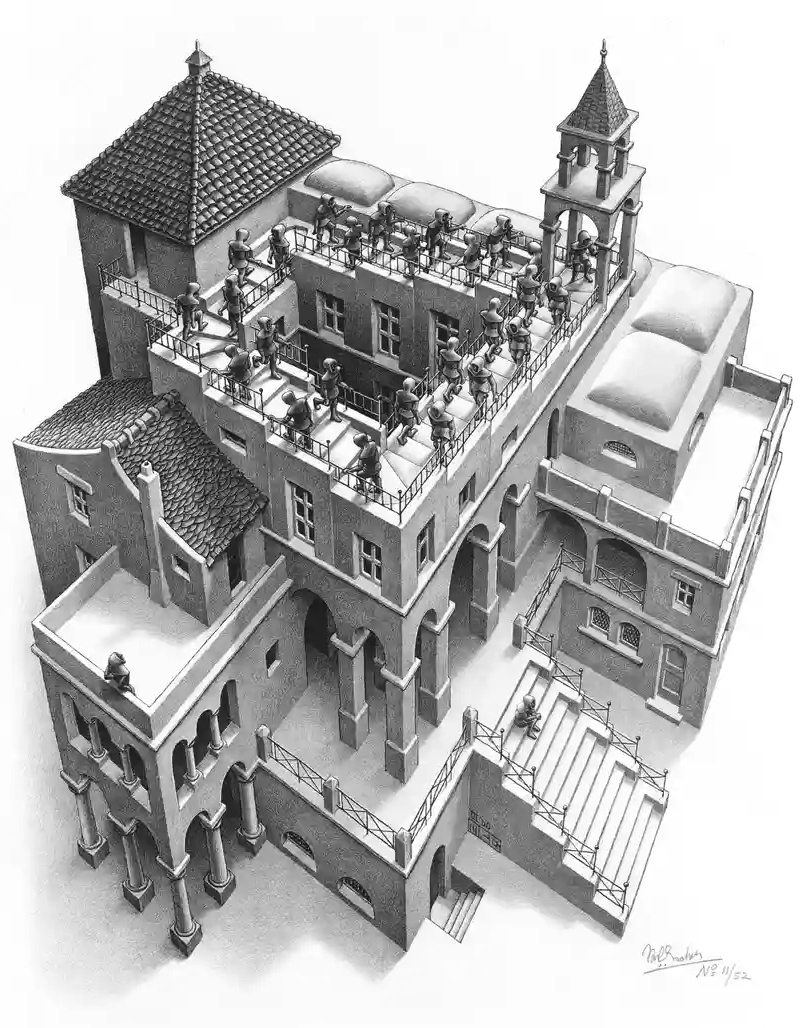
\includegraphics[width=1.05\columnwidth]{figures/penrose-stairs.png}
	\caption{
		\emph{``Ascending and Descending'' by M.\ C.\ Escher, 1960} --- perhaps the most famous illustration of an inexact $2$-form (the slope of the stairs) and its inconsistent `integral' (the impossible staircase).
	}
\end{marginfigure}
We can also translate the involutivity condition from tangent subbundles to ideals.
\begin{theorem}
	\label{thm:dual-involutive}
	If $𝒟 ⊆ \TTℳ$ is a tangent subbundle and $I ⊆ \forms[1](ℳ)$ is its associated ideal, then
	\begin{align}
		[𝒟, 𝒟] ⊆ 𝒟
		\quad ⟺ \quad
		\text{$𝒟$ is involutive}
		\quad ⟺ \quad
		\dd I ⊆ I
	.\end{align}
\end{theorem}
\begin{proof}
	The first equivalence is by definition, included for readability.
	For the second, note that the ideal $I$ is generated by $1$-forms $ω$ which vanish on $𝒟$.
	That is, $ω(𝒖) = 0$ for all $𝒖 ∈ \secs(𝒟)$, so if $𝒖, 𝒗 ∈ \secs(𝒟)$ then
	\begin{align}
		\label{eqn:xd-lb-identity}
		\dd ω(𝒖, 𝒗) &= 𝒖\qty(ω(𝒗)) - 𝒗\qty(ω(𝒖)) - ω([𝒖, 𝒗])
	\\	&= - ω([𝒖, 𝒗])
	,\end{align}
	since $ω(𝒖) = ω(𝒗) = 0$.
	If $𝒟$ is involutive then $[𝒖, 𝒗] ∈ \secs(𝒟)$ and $\dd ω(𝒖, 𝒗) = 0$.
	Thus, $\dd ω ∈ I$ if and only if $𝒟$ is involutive.
\end{proof}

Hence, by \cref{thm:Frobenius,thm:dual-involutive}, a tangent subbundle admits maximal integral surfaces if and only if its associated ideal $I$ is closed under exterior differentiation, $\dd I ⊆ I$.

Stokes’ \cref{thm:flat-stokes} states that a differential form $φ$ is integrable if it is exact (i.e., if $φ = \dd ϕ$).
On a contractible domain, this is equivalent to $φ$ being closed, by Poincaré's lemma.
In the same vein, \cref{thm:dual-involutive} states that an exterior differential system is integrable over a contractible domain if and only if its associated ideal is closed.




\subsection{Curvature as an obstruction to integrability}




We may employ Frobenius’ theorem to find the integrability condition for the connection on a vector bundle $\fibrebundle V 𝒱 ℳ$.
A linear Ehresmann connection $H$ is integrable if there exist maximal integral manifolds $f ∈ \secs(ℱ)$ which are everywhere horizontal, $\TT_p f = H_p$.
This means that $∇ f = 0$ everywhere, that parallel transport is path-independent, and that loop holonomy is always trivial.

Elaborating the condition $∇ f = 0$, we have
\begin{align}
	\label{eqn:covariantly-const}
	∇_𝒖 X = 𝒖(X) + Γ(𝒖)X = 0
	\qqtext{or}
	∂_μ X^a = -Γ_μ{}^a{}_b X^b
\end{align}
everywhere for all $𝒖 ∈ \TT ℳ$.
These equations describe the tangent subbundle $H$.
To express this, introduce coordinates $\set{x^μ}$ of $ℳ$ and linear coordinates $\set{x^a}$ of $V$ with respect to some basis.
A point $X ∈ 𝒱$ is a base point $π(X) ≡ (X^μ) ∈ ℳ$ together with a fibre value $(X^a) ∈ V$, having total coordinates
\begin{math}
	X = (X^μ, X^a)
.\end{math}
Similarly, a vector in $\TT_X 𝒱$ has components
\begin{math}
	δX = (δX^μ, δX^a)
.\end{math}

Such a vector $δX ∈ \TT_X 𝒱$ satisfies \cref{eqn:covariantly-const} if $δX^a/δX^μ = -Γ_μ{}^a{}_b X^b$, and hence the Ehresmann connection may be expressed as
\begin{align}
	\label{eqn:parallel-transport-tangent-subbundle}
	H_X = \spanof{(δX^μ, -Γ_μ{}^a{}_b X^b δX^μ) | (δX^μ) ∈ \TT_Xℳ}
\end{align}
for each $X ∈ 𝒱$.
Geometrically, this describes the change in vector components $δX^a$ induced by a nudge in the base point $δX^μ$ if $X$ is constrained to move along $H$.

To employ Frobenius’ theorem, we will find a dual representation of \cref{eqn:parallel-transport-tangent-subbundle} in terms of forms.
Any $X ∈ H$ is of the form
\begin{align}
	X = δX^μ(\∂_μ - Γ_μ{}^a{}_b X^b \∂_a)
.\end{align}
If $I$ is the ideal associated to $H$, then any $1$-form $\df ω ∈ I$ satisfies
\begin{align}
	\df ω(X) = δX^μ\qty(ω_μ - Γ_μ{}^a{}_b X^b ω_a) = 0
\end{align}
where $ω_A ≔ \df ω(\∂_A)$, implying $ω_μ =  Γ_μ{}^a{}_b X^b ω_a$ at $X$.
Written in the coordinate dual basis $\set{\df{\dd X}^μ, \df{\dd X}^a} ⊂ \TT^* 𝒱$,
\begin{align}
	\label{eqn:arbitrary-1-form-gen}
	\df ω = ω_a\qty(\df{\dd X}^a + Γ_μ{}^a{}_b X^b \df{\dd X}^μ)
\end{align}
where $ω_a$ are free scalar parameters.
Here, we adopt the notation `$\df{\phantom{ω}}$' to label differential forms for clarity.
Since \cref{eqn:arbitrary-1-form-gen} is a general $1$-form of the ideal $I$, we can see that $I$ is generated by the $1$-forms
\begin{align}
	\label{eqn:ideal-gens}
	\df Ω^a = \df{\dd X}^a + \df Γ^a{}_b X^b
,\end{align}
where we define the connection $1$-forms $\df Γ^a{}_b ≔ Γ_μ{}^a{}_b \, \df{\dd X}^μ$.

The dual formulation of Frobenius’ theorem (\cref{thm:dual-involutive}) states that the tangent subbundle $H$ is involutive if and only if the ideal $I$ is closed.
This means that $\dd \df Ω^a ∈ \dd I$ for every generator, which is equivalent to the condition $\dd\df Ω^a = \df α_a ∧ \df Ω^a$ for arbitrary `component $1$-forms' $\df α_a$.
By direct calculation,
\begin{align}
	\dd\df Ω^a &= \df{\dd^2 X^a} + \dd \df Γ^a{}_b X^b - \df Γ^a{}_b ∧ \df{\dd X^b}
\\	&= (\dd \df Γ^a{}_b + \df Γ^a{}_c ∧ \df Γ^c{}_b) X^b - \df Γ^a{}_b ∧ \df Ω^a
\end{align}
where we substitute \cref{eqn:ideal-gens} on the second line.
Therefore, $\dd\df Ω^a ∈ I$ if and only if the residual term, called the \textdef{connection $2$-form}
\begin{align}
	\label{eqn:curvature-2-form}
	\df R^a{}_b ≔ \dd \df Γ^a{}_b + \df Γ^a{}_c ∧ \df Γ^c{}_b
,\end{align}
vanishes.
These $\df R^a{}_b$ measure the obstruction to integrability of the covariant derivative, and are identified as the primary object describing the connection's curvature.



\section{Stokes' Theorem for Curvature 2-forms}

Another way of showing that parallel transport is path-independent if and only if the curvature \eqref{eqn:curvature-2-form} vanishes is by relating the holonomy of a loop to the curvature across a surface bounded by the loop.

% This is done by deriving a Stokes-like theorem for the special case of a connection $1$-form, using a
% \begin{align}
% 	\text{``} \int_Σ \df R = \oint_{∂Σ} \df Γ \text{''}
% \end{align}


\subsection{Path-ordered exponentiation}

An initial value problem of the form
\begin{align}
	\label{eqn:path-ordered-exp-ode}
	\dv{U(t)}{t} = A(t)U(t)
\end{align}
with $U(0)$ given has the solution
\begin{align}
	U(t) = e^{\int_0^t dτ A(τ)} \, U(0)
\end{align}
provided that $A(t)$ commutes with itself at all other times, $[A(t), A(s)] = 0$.
If $A(t)$ is not necessarily commutative, then the solution may still be written formally in the following way.

By a first-order Taylor expansion, the value after an infinitesimal time-step $dt$ step is
\begin{align}
	U(dt) = U(0) + ∂_tU(0)dt = (1 + A(0)dt)U(0) = e^{A(0)dt} \, U(0)
.\end{align}
The value at a finite time $t$ is then recovered by composing steps as above, forming the \textdef{path-ordered exponential}
\begin{align}
	\label{eqn:path-ordrered-exp-solution}
	U(t)U^{-1}(0) = \Pexpl[τ]\int_0^t dτ A(τ) ≔ \lim_{dt → 0} \prod_{t_i}^{t←0} e^{A(t_i)dt}
,\end{align}
where the product $\prod_{t_i}^{t←0}$ is over values $t ≥ t_i ≥ 0$ in steps of $dt$ where each exponential factor appears \emph{right-to-left} in order of increasing $t_i$.



From the observation that $∂_t(U(t)U^{-1}(t)) = 0$ we obtain the `inverse' of the original differential equation,
\begin{align}
	\label{eqn:path-ordered-exp-ode-inv}
	∂_tU(t)^{-1} = -U(t)^{-1}A(t)
,\end{align}
which is identical to \eqref{eqn:path-ordered-exp-ode} only transposed and substituting $U(t)^T \mapsto U(t)^{-1}$ and $A(t)^T \mapsto -A(t)$.
Hence, \eqref{eqn:path-ordered-exp-ode-inv} has solution
\begin{align}
	U(t)^{-1} &= U(0)^{-1}\Pexpr[τ]\int_0^t dτ (-A(τ))
\\	&= U(0)^{-1}\Pexpl[τ]\int_t^0 dτ A(τ)
.\end{align}
Hence, the left-to-right ordered exponential $\Pexpr$ is the same as a right-to-left $\Pexpl$ if the endpoints $0 ↔ t$ are swapped and the integrand $dτ \mapsto -dτ$ flips sign.

\subsubsection{The transport operator as a path-ordered exponential}

The transport operator satisfies the differential equation \eqref{eqn:trans-ode}, which for a linear connection is of the form \eqref{eqn:path-ordered-exp-ode}.
Therefore, using the initial data $\trans_{γ(0 ← 0)} = \op{id}$, \cref{eqn:trans-ode} may be solved explicitly by
\begin{align}
	\label{eqn:trans-pexp}
	\trans_{γ(s ← 0)} = \Pexpl\int_γ (-\df Γ) = \Pexpr\int_s^0 ds \, \df Γ_{\vb{\dot γ(s)}}
.\end{align}
% \Cref{eqn:trans-pexp} is the solution to \cref{eqn:trans-ode} along $γ$ with the initial data $\trans_{γ(0 ← 0)} = \op{id}$.



\subsection{Surface-ordered exponentiation}




\begin{theorem}[Stokes theorem for curvature $2$-forms]
	\label{thm:nast}
	Let $γ : [0, 1] → ℳ$ be a contractable loop with start and end point $p$.
	Let $h_λ$ be a contraction homotopy with $λ ∈ [0, 1]$ so that $h_0(x) = p$ and $h_1(x) = x$.
	Define $ξ(λ, s) ≔ h_λ(γ(s))$ as the surface swept out by $γ$ under the contraction.
	
	\begin{marginfigure}
		\includefigure[1.1\columnwidth]{homotopy}
		\caption{
			The curve $γ$ and the surface of homotopy $ξ$.
			The bold curve represents the portion of $h_λ \circ γ$ from parameter value $0$ to $s$.
		}
	\end{marginfigure}

	Let $\df Γ$ be a connection $1$-form and let $U(λ, s) ≔ \trans_{ξ(λ, s ← 0)}$ be the group element resulting from parallel transport along the path $ξ(λ, s ← 0)$.
	Then,
	\begin{align}
		\trans_{γ}
		&= \Pexpl[s]\int_γ (-\df Γ )
	\\	&= \Pexpr[λ]\int_0^1 dλ \int_0^1 ds \; U^{-1} \, \df R(∂_s ξ, ∂_λ ξ) \, U
	,\end{align}
	where $\df R = \dd\df Γ + \df Γ ∧ \df Γ$ is the curvature $2$-form.
	Note that $U ≡ U(λ, s)$ and $ξ ≡ ξ(λ, s)$.

	\toself{This awkwardly uses different path orderings. Bralić's is left-to-right.}
\end{theorem}

\begin{proof}
	Define the abbreviations
	\begin{align}
		Γ_λ &≔ \df Γ(∂_λ ξ)
	&	&\text{and}
	&	Γ_s &≔ \df Γ(∂_s ξ)
		\label{eqn:nast-working-shorthand}
	,\end{align}
	noting that $λ$ and $s$ are \emph{not} indices.
	In full component form, these would be written, e.g.,
	\begin{align}
		(Γ_λ)^a{}_b \, |_{ξ(λ, s)} = Γ_μ{}^a{}_b \, |_{ξ(λ, s)} \pdv{ξ^μ(λ, s)}{λ}
	.\end{align}
	From \cref{lem:dtrans-is-hlift}, we have
	\begin{align}
		\eval{\pdv{U(λ, s)}{s}}_{s = 0} = \dv{s} \eval{\trans_{ξ(λ, s ← 0)}}_{s = 0} = - \df Γ(∂_s ξ)
	\end{align}
	where $ξ ≡ ξ(λ, s)$, which implies
	\begin{align}
		∂_s U &= -Γ_s \, U
	&	&\text{and}
	&	∂_s U^{-1} &= U^{-1}Γ_s
	\end{align}
	where $U ≡ U(λ, s)$.
	From these two relations it follows easily that
	\begin{align}
		\label{eqn:nast-working.1}
		∂_s\qty(U^{-1}∂_λ U)
	&=	U^{-1}\qty(Γ_s ∂_λ U + ∂_λ∂_sU)
	=	-U^{-1} (∂_λ Γ_s) \, U
	\\\qqtext{and}	∂_s(U^{-1}Γ_λU)
	&=	U^{-1}(Γ_sΓ_λ + ∂_sΓ_λ - Γ_λΓ_s)U
	.\end{align}
	The sum of the two equations above is
	\begin{align}
		∂_s(U^{-1}(∂_λ + Γ_λ)U) = U^{-1}(∂_s Γ_λ + Γ_s Γ_λ - (s ↔︎ λ)) \, U
	.\end{align}
	Note that
	\begin{math}
		∂_s Γ_λ = ∂_s(Γ_μ(∂_λ ξ)) = (∂_s Γ_μ) ∂_μ ξ^μ + Γ_μ \, ∂_s∂_λ ξ^μ
	\end{math}
	and similarly for $∂_λ Γ_s$, so that mixed partial derivatives cancel, leaving
	\begin{align}
		∂_s Γ_λ - ∂_λ Γ_s = (∂_s \df Γ)(∂_λ ξ) - (∂_λ \df Γ)(∂_s ξ)
	.\end{align}
	Putting this together, we have
	\begin{align}
		∂_s(U^{-1}(∂_λ + Γ_λ)U)
		&= U^{-1} \qty((∂_s \df Γ)(∂_λ ξ) + \df Γ(∂_s ξ)\df Γ(∂_λ ξ) - (s ↔︎ λ)) \, U
	\\	&= U^{-1} (\dd\df Γ + \df Γ ∧ \df Γ)(∂_s ξ, ∂_λ ξ) \, U
	\\	&= U^{-1} \df R(∂_s ξ, ∂_λ ξ) \, U
		\label{eqn:nast-working.2}
	.\end{align}

	Recall that $U$ and $U^{-1}$ are the group elements which parallel transport vectors along $ξ(λ, s ← 0)$ and back again, respectively.
	Also, note that $\df R$ is a $\liealg{gl}(\manif V)$-valued $2$-form, which acts to infinitesimally transform vectors in $𝒱$.
	With these in mind, it is clear that \cref{eqn:nast-working.2} is an infinitesimal linear map from the fibre $𝒱_p$ to itself.\sidenote{
		Imagine the right-hand side of \cref{eqn:nast-working.2} acting on a vector $X$.
		First, $X$ is transported by $U$ from $ξ(λ, 0) = p$ to $ξ(λ, s)$, then transformed infinitesimally by $\df R$, and finally transported back to the fibre at $p$ by $U^{-1}$.
	}
	Thus, it is well-defined to integrate \cref{eqn:nast-working.2} with respect to $s$, to obtain a finite linear transformation on $𝒱_p$.
	% We will find that this is exactly the holonomy around $h_λ γ$.

	Integrating the left-hand side of \cref{eqn:nast-working.2} yields
	\begin{align}
		\label{eqn:nast-working.3}
		\int_0^1 ds \, U^{-1}(λ, 1)(∂_λ + Γ_λ)U(λ, 1)
		= U^{-1}(λ, 1) ∂_λ U(λ, 1)
	\end{align}
	since $Γ_λ = \df Γ(∂_λ ξ(λ, s))$ vanishes at $s ∈ \set{0, 1}$ because $ξ(λ, 0) = ξ(λ, 1) = p$ is constant.
	Thus, integrating both sides yields
	\begin{align}
		U^{-1}(λ, 1) ∂_λ U(λ, 1)
		= \int_0^1 ds \, U^{-1} \df R(∂_s ξ, ∂_λ ξ) \, U
	.\end{align}
	This is an initial value problem of the form $∂_λ U(λ, 1) = U(λ, 1)A(λ)$, whose solution at $λ = 1$ may be given as the path-ordered exponential
	\begin{align}
		U(1, 1) = U(1, 0) \Pexpr\int_0^1 dλ \, A(λ)
	\end{align}
	where $A(λ)$ is the right-hand side of \cref{eqn:nast-working.3}.
	Since $U(1, 1) = \trans_γ$ and $U(1, 0) = \op{id}$, this shows the right-hand side of the theorem.
\end{proof}


\begin{corollary}
	Parallel transport is path-independent if and only if curvature vanishes everywhere.
\end{corollary}
\begin{proof}
	If the curvature vanishes everywhere, then by \cref{thm:nast} the holonomy around any loop is trivial, implying the transport operator between two fixed points is path-independent.

	Conversely, if parallel transport is path-independent, then the transport operator around any loop $γ$ is the identity.
	By \cref{thm:nast}, this implies that the total curvature on a surface bounded by $γ$ is zero.
	But since the surface and loop are arbitrary, the curvature must vanish everywhere.
\end{proof}



\chapter{Conclusions}

\todo{
	Highlight \emph{original} findings of \cref{part:1,part:2}:
	\begin{itemize}
		\item BCHD formula for spacetime
		\item Geometric Lie derivative formula for multivectors
	\end{itemize}
	Not original but still of interest:
	\begin{itemize}
		\item Bivector connection and the bivector-valued Riemann $2$-form.
		\item Stokes' theorem for curvature $2$-form (non-Abelian Stokes)
	\end{itemize}
}

\appendix


\chapter{Integral Theorems}


\section{Stokes' theorem for exterior calculus}

\begin{theorem}[Stokes' theorem in $\RR^n$]
	\label{thm:flat-stokes}
	If $R ⊆ \RR^n$ is a compact $k$-dimensional hypersurface with boundary $∂R$, then a smooth differential form $ω ∈ \forms[k - 1](R)$ satisfies
	\begin{align}
		\label{eqn:stokes}
		\int_R \dd ω = \int_{∂R} ω
	.\end{align}
\end{theorem}
\begin{proof}
	Since $R$ is a $k$-dimensional region with boundary, every point $x ∈ R$ has a neighbourhood diffeomorphic to a neighbourhood of the origin in either $\RR^k$ or $H^k ≔ [0, ∞) ⊕ \RR^{k - 1}$, depending on whether $x$ is an interior point or a boundary point, respectively.

	\begin{marginfigure}
		\includefigure[\columnwidth]{stokes-theorem}
		\caption{
			Neighbourhoods in $R$ are diffeomorphic either to interior balls or boundary half-balls.
		}
		\label{fig:stokes-theorem}
	\end{marginfigure}

	Let $\set{U_i}$ be a cover of $R$ consisting of such neighbourhoods.
	Since $R$ is compact, we may assume $\bigcup_{i=1}^N \set{U_i} = R$ to be a finite covering.
	Thus, we have finitely maps $h_i : U_i → X$ where $X$ is either $\RR^k$ or the half-space $H^k$, where $U_i \cong h_i(U_i)$ are diffeomorphic (see \cref{fig:stokes-theorem}).

	Finally, let $\set{ϕ_i : R → [0, 1]}$ be a partition of unity subordinate to $\set{U_i}$, so that $\set{x ∈ R | ϕ_i(x) > 0} ⊆ U_i$ and $ω = \sum_{i=1}^N ϕ_iω$.
	We need only prove the equality \eqref{eqn:stokes} for each $ω_i ≔ ϕ_iω$, and the full result follows be linearity.
	
	The form $h_i^*ω_i ∈ \forms[k - 1](X)$ can be written with respect to canonical coordinates of $X$ as
	\begin{align}
		h_i^*ω_i = \sum_{j=1}^k f_j (-1)^{j - 1} \dd x^{1\cdots\hat{j}\cdots k}
	\end{align}
	using the multi-index notation $\dx^{\etc{i_\i}{}k} ≡ \etc{\dx^{i_\i}}∧k$, where the hat denotes an omitted term.
	The factor of $(-1)^{j - 1}$ gives the $(k - 1)$-form the boundary orientation induced by the volume form $\dx^{\etc\i{}k}$ for convenience.
	Since pullbacks commute with $\dd$,
	\begin{align}
		h^*\ddω_i = \dd(h_i^*ω_i) = \sum_{j=1}^k \pdv{f_j}{x^j} \dd x^{1\cdots n}
	.\end{align}
	There are then two cases to consider.
	\begin{itemize}
		\item \emph{Interior case.}
		If $h_i : U_i → \RR^k$, then the right-hand side of \cref{eqn:stokes} vanishes because $ω_i$ is zero outside the neighbourhood $U_i ⊂ R$ which nowhere meets the boundary $∂R$.
		\begin{align}
			\int_{∂R} ω_i = \int_{∂U_i} ω_i = \int_∅ ω_i = 0
		\end{align}
		The left-hand side evaluates to
		\begin{align}
			\int_R \dd ω_i
			&= \int_X \dd (h_i^*ω_i)
			= \int_{\RR^k} \sum_{j=1}^k \pdv{f_j}{x^j} \dd x^{1\cdots n}
		\\	&= \underbrace{\etc{\int_{-∞}^{+∞}}{}{}}_k \sum_{j=1}^k \pdv{f_j}{x^j} \etc{dx^\i}{}{k}
		\\	&= \underbrace{\etc{\int_{-∞}^{+∞}}{}{}}_{k - 1} \sum_{j=1}^k \eval{f_j}_{x^j=-∞}^{+∞} (-1)^{j-1} dx^1\cdots\widehat{dx^j}\cdots dx^k
			= 0
		,\end{align}
		which vanishes because $h_i^*ω_i$, and hence the $f_j$, vanish outside the neighbourhood $h_i(U_i) ⊂ \RR^k$.

	\item \emph{Boundary case.}
	If $h_i : U_i → H^k$, then the boundary $∂U_i ⊂ ∂R$ is mapped onto the hyperplane $∂H^k = \set{(0, \etc[2]{x^\i},k) | x^j ∈ \RR}$.
	Thus, $dx^1 = 0$ on this boundary, and the right-hand side of \cref{eqn:stokes} becomes
	\begin{align}
		\int_{∂R}ω_i
		&= \int_{∂U_i} h_i^*ω_i
		= -\int_{\RR^{k - 1}} f_1 \etc[2]{dx^\i}{}k
	\\	&= -\underbrace{\etc{\int_{-∞}^{+∞}}{}{}}_{k - 1} f_1(0, \etc[2]{x^\i},k) \etc[2]{dx^\i}{}k
	.\end{align}
	The factor of $-1$ comes from the induced orientation of the boundary $∂H^k$, which is outward-facing, so in the \emph{negative} $x^1$ direction.
	For the left-hand side of \cref{eqn:stokes},
	\begin{align}
		\int_R \dd ω_i
		&= \int_{H^k} h_i^*\ddω_i
		= \int_0^∞ \etc{\int_{-∞}^{+∞}}{}{} \sum_{j=1}^k \pdv{f_j}{x^j} \etc{dx^\i}{}k
	\intertext{
		All terms $\pdv{f_j}{x^j}dx^j$ in the sum for $j > 1$ integrate to boundary terms $x_j → ±∞$ where $f_j$ vanishes.
		This leaves the single term from the integration of $dx^1$,
	}
		&= -\etc{\int_{-∞}^{+∞}}{}{} \eval{f_1}_{x^1=0}^∞ \etc[2]{dx^\i}k
	.\end{align}

	\end{itemize}

	Thus, we have equality for all $ω_i$, so
	\begin{align}
		\int_R \dd ω = \sum_{i=1}^N \int_R \dd ω_i = \sum_{i=1}^N \int_{∂R} ω_i = \int_{∂R} ω
	\end{align}
	by linearity.
\end{proof}

\section{Fundamental theorem of geometric calculus}

\begin{theorem}
	Let $f(𝒙)$ be a multivector field.
	The vector derivative is
	\begin{align}
		\vd f(𝒙) = \lim_{|ℛ| → 0} \frac1{|ℛ|\vol} \oint_{∂ℛ} \bd S f
	,\end{align}
	where $ℛ$ is a volume containing $𝒙$ with boundary $∂ℛ$ and volume $|ℛ| = \int_ℛ \bd V$.
	The limit is taken as the volume $ℛ$ shrinks to the point $𝒙$.
\end{theorem}
Note that the integrand $\bd S f$ is the geometric product between the hypersurface element and the field.
\begin{proof}
	It will suffice to prove the case where $ℛ$ is a box shape; arbitrary regions can be approximated via tessellation in the limit of vanishing voxel size.

	Let $B_ε = \set{x^i\ve_i | x^i ∈ [-ε, +ε]}$ denote the $n$-dimensional cube of diameter $2ε$ centred at the origin.
	If the surface $∂B_ε$ is oriented outward, then the face in the $+\ve^k$ direction is orientated like the $(n-1)$-blade $\vol \ve^k = (-1)^{n-k}\etcskip{\ve_\i}∧kn$.
	Upon this face the infinitesimal surface element is
	\begin{align}
		% \bd^{(k)}x = \vol \ve^k dx^1\cdots\widehat{dx^k}\cdots dx^n
		\bd^{(k)}x = \vol \ve^k \etcskip{dx^\i}{}{k}{n}
	,\end{align}
	while the opposing face has surface element $-\bd^{(k)}x$.

	Consider the integral of $f$ over the surface $∂B_ε$, split into a sum of $n$ surface integrals over each pair of opposing faces.
	The $k$th pair are the surfaces $\set{x^i\ve_i ± ε\ve_k | x^i ∈ [-ε, +ε], i ≠ k}$ where $i$ sums over axes \emph{other} than $k$.
	Hence, we have
	\begin{align}
		\oint_{∂B_ε} \bd S f = \sum_{k=1}^n \int_{[-ε, +ε]^{n-1}} \bd^{(k)}x \, \qty(f(x^i\ve_i + ε\ve_k) - f(x^i\ve_i - ε\ve_k))
	,	\quad(i ≠ k)
	.\end{align}
	By series expanding $f$ in each $x^i$, and then in $ε$, obtain
	\begin{align}
		f(x^i\ve_i ± ε\ve_k) &= f(±ε\ve_k) + x^i ∂_{\ve^i} (f(0) ± ε∂_{\ve^k} f(0))
	.\end{align}
	Since $|x^i| ≤ ε$, the last term is $𝒪(ε^2)$, and difference in the integrand is hence
	\begin{align}
		f(x^i\ve_i + ε\ve_k) - f(x^i\ve_i - ε\ve_k)
		&= f(ε\ve_k) - f(-ε\ve_k) + 𝒪(ε^2)
	\\	&= 2ε∂_{\ve^k}f(0) + 𝒪(ε^2)
	.\end{align}
	Therefore, after pulling constants outside the integrals, we have
	\begin{align}
		\oint_{∂B_ε} \bd S f
		&≈ \sum_{k=1}^n 2ε \, ∂_{\ve^k} f(0) \int_{[-ε, +ε]^{n-1}} \bd^{(k)}x
	\end{align}
	to order $𝒪(ε^2)$.
	The integrands each evaluate to the area $(2ε)^{n-1}$, giving
	\begin{align}
		\oint_{∂B_ε} \bd S f
		≈ (2ε)^n \vol\ve^k ∂_{\ve^k} f(0)
		= |B_ε|\vol \, \vd f(0)
	,\end{align}
	to order $𝒪(ε^2)$, which becomes exact in the limit,
	\begin{align}
		\label{eqn:vd-int-form}
		\vd f(0) = \lim_{ε → 0} \frac1{|B_ε|\vol} \oint_{∂B_ε} \bd S f
	.\end{align}

	By translation, $f(𝒙) ↦ f'(𝒙) = f(𝒙 - 𝒖)$, we obtain the integral form of $\vd f(𝒖)$ evaluated at an arbitrary position $𝒖$.
\end{proof}

\begin{theorem}
	For an $n$-dimensional region $ℛ$ with boundary $∂ℛ$, and a multivector field $f(𝒙)$,
	\begin{align}
		\int_ℛ \bd V \, \vd f = \oint_{∂ℛ} \bd S f
	,\end{align}
	where $\bd V$ denotes an $n$-blade volume element, and $\bd S$ an $(n - 1)$-blade surface element, and where juxtoposition is the geometric product. 
\end{theorem}
\begin{proof}
	An arbitray volume $ℛ$ with boundary $∂ℛ$ can be approximated as tessellated boxes of arbitrily small size.\sidenote{
		It is not neccesary that the surface area of the approximation converge to $|∂ℛ|$.
	}
	Suppose $ℛ$ is approximated by a regular lattice of $N$ boxes of radius $ε$.
	Consider the sum of $\vd f$ over the lattice points, weighted by volume.
	From \cref{eqn:vd-int-form} this can be written in terms a sum of surface integrals,
	\begin{align}
		\sum_{i=1}^N |B_i|\vol \, \vd f(𝒙_i) = \sum_{i=1}^N \oint_{∂B_i} \bd S f
	.\end{align}
	Note that interior faces of the boxes come in oppositely-oriented pairs, so that surface integrals over interior faces cancel.
	Therefore, the result is obtained in the continuous limit $N → ∞$.
\end{proof}

\todo{Comment on how this generalizes Stokes' theorem.}

\newgeometry{margin=3.5cm}

\small
\bibliography{references}

\end{document}